\documentclass[12pt,a4paper]{article}
\usepackage[margin=24mm]{geometry}
\usepackage[T1]{fontenc}\usepackage[utf8]{inputenc}\usepackage{lmodern,microtype}
\usepackage{graphicx,longtable,booktabs,array,amsmath,hyperref,fancyhdr,xurl}
\hypersetup{colorlinks=true,linkcolor=black,citecolor=black,urlcolor=blue}
\setlength{\parindent}{0pt}\setlength{\parskip}{6pt}\setlength{\emergencystretch}{3em}
\renewcommand{\arraystretch}{1.18}\pagestyle{fancy}\fancyhf{}\fancyhead[L]{\small GPU sharing for multi-tenant inference}\fancyhead[R]{\small Task 3 draft}\fancyfoot[C]{\thepage}\setlength{\headheight}{15pt}
\begin{document}
\begin{titlepage}\centering
{\large NED University of Engineering and Technology\\Department of Software Engineering\par}\vspace{28mm}
{\LARGE\bfseries GPU Sharing for Multi-Tenant Inference\par}\vspace{6mm}
{\Large A Bounded Systematic Evidence Synthesis of Performance, Isolation and Engineering Trade-offs\par}\vspace{20mm}
{\large Operating Systems CEP -- Topic 23\\Task 3: Complete First Draft\par}\vspace{16mm}
Eshaal Faisal (SE-24008)\\Raazia Imran Reshamwala (SE-24009)\\Rameen Siddiqui (SE-24016)
\vfill 23 October 2026\\[6mm]
\small Working corpus: 31 report versions, 30 unique studies.\\Frozen submission: 21 reports, 20 studies, preserved separately.\\The bounded selection and remaining verification work are explicitly reported.
\end{titlepage}
\begin{abstract}
GPU sharing for multi-tenant inference requires a choice among resource efficiency, request latency, isolation and implementation cost. This working review synthesizes 30 studies represented by 31 reports. The imported search register contains 4,189 occurrences and 4,075 canonical records after 114 duplicate links. In the continued 559-record branch, title/abstract screening excluded 225 records and advanced 334; 10 additional studies met full-text eligibility, 4 reports were excluded at full text, and 320 advanced records await eligibility or identity closure. These branch counts do not constitute a reconciled final whole-review PRISMA flow. The analysis uses 300 appraisal items, 90 reported observations and two transparent calculations. It combines temporal scheduling, software spatial sharing, hardware partitions, runtime/API mediation, model-memory management and hybrid controls. The evidence supports conditional selection: fine-grained control can protect request latency, while model modification, profiling, transfer bandwidth and shared-context faults constrain its use. No pooled effect or universal winner is supported. The conclusions remain limited by incomplete selection, historical search-provenance gaps, title-only screening and source-version uncertainty.
\end{abstract}
\tableofcontents\clearpage
\section{Introduction}
\subsection{Background and engineering problem}
GPU sharing for inference is an operating-system resource-management problem: several services compete for finite execution capacity, device memory and access to a runtime that may not expose the control required by a service-level objective. Increasing concurrent execution can improve aggregate work completed while worsening the response of an individual service. Conversely, reserving the entire accelerator for one model can simplify interference management but leaves less opportunity to use spare capacity. The engineering question is therefore conditional: which mechanism should be selected for a particular workload, latency objective, memory requirement and isolation boundary?

The evidence makes this tension concrete. The ParvaGPU manuscript reports a local configuration in which throughput increases from 354 to 446 requests/s as the number of MPS processes rises from one to three, while reported latency increases from 11 to 27 ms. These outcomes move in opposite desirable directions. The latency quantile is unspecified, so the example cannot establish a P99 service guarantee. XSched instead reports a foreground P99 ratio of 1.07 relative to standalone execution, compared with 1.53 for native Triton in the recorded configuration. These are different engineering objectives, not numbers on one ranking scale \cite{P011,P015}.

\subsection{Scope and contribution}
The unit of technical interpretation is concurrent inference on one physical GPU. A multi-GPU or cluster paper contributes only where a local sharing result can be separated from fleet scheduling. Mixed inference/training papers contribute inference outcomes and the associated background-work cost. Training throughput is not relabeled as inference throughput. Non-GPU accelerator results in otherwise relevant papers are outside the primary comparison.

This working draft integrates the frozen 20-study/21-report corpus with 10 source-eligible additions, giving 30 studies represented by 31 reports. Its contribution is a decision-oriented comparison that joins mechanisms, evaluation conditions, reported outcomes, implementation costs and limitations. Existing surveys already examine multi-tenant GPU inference, accelerator-sharing efficiency/fairness/security, and GPU-datacenter scheduling \cite{surveyYu,surveyHuang,surveyYe}. The present taxonomy is therefore an organizational tool, not a first-survey claim. Its narrower emphasis is local GPU outcome traceability, comparability, source-version boundaries and conditional engineering decisions, including relevant 2025 systems. The survey audit records accessed versions and unavailable contextual leads; it does not establish exhaustive novelty. It distinguishes performance interference, resource partitioning, memory protection and fault containment. It also retains adverse outcomes rather than selecting only favorable headline speedups.

The review is not an exhaustive census of the search results. All 559 records in the continuation branch now have a title/abstract-stage decision: 225 exclusions and 334 advancements. 10 additions and 4 full-text exclusions are resolved; 320 advanced records still await eligibility or report-identity closure. This draft supports candidate selection under observed conditions while the wider coverage question remains open.

\subsection{Objectives}
The objectives are to classify the available mechanisms by their actual control boundaries; determine which outcomes are comparable; explain the conditions behind benefits and regressions; and derive recommendations that identify both expected benefit and sacrifice. The review does not seek a universal winning system. It seeks an auditable reason for choosing a candidate under stated constraints.

\section{Research questions}
The following research questions reproduce the submitted Task 1 protocol (Table 3).
\begin{description}
\item[RQ1] What time-slicing, MPS, MIG and API remoting mechanisms are evaluated for concurrent inference on one GPU, and how do sharing granularity, layer and isolation boundary classify them?
\item[RQ2] How do studies measure utilization, throughput, density, average/tail latency, predictability and interference, and how comparable are their experimental methods?
\item[RQ3] Under what GPU, workload, batch, tenant mix and configuration conditions are changes in utilization, throughput, density and latency reported?
\item[RQ4] What resource and fault isolation properties, trade-offs, implementation costs and conflicting results are reported, and what limits the evidence?
\item[RQ5] Which approach or combination is supported for specified inference-serving conditions and priorities, with what confidence and alternatives?
\end{description}

\section{Research methodology}
\subsection{Protocol and implemented method}
The submitted Task 1 protocol is preserved unchanged in the repository. It specifies independent screening and appraisal, stable record/report/study identifiers, page-level extraction and a condition-aware narrative synthesis. This draft follows its conceptual comparison rules while explicitly reporting deviations in execution. PRISMA supplies the reporting framework, while the search audit preserves the executed queries rather than replacing them with planned expressions \cite{prisma,prismas,kitchenham}.

The supplied Task 2 workbook is the source of the current corpus and historical decisions. GitHub's preceding status described an earlier 15-form assessment. Importing the newer workbook does not mean those older registers were silently rewritten. Task 3 stores the uploaded baseline separately and keeps the inherited research history available.

The implemented review uses a source-based assessment under team direction. No independent human item-level votes or calibration are inferred. Activity records preserve actual preparation and decision times, which do not establish when a person reviewed a record.

\subsection{Integrated source review of all included studies}
The frozen source-review packages cover the original 20 studies and the REEF companion report: 70 appraisal items and 30 outcomes for Eshaal's allocation, 70 appraisal items and 13 outcomes for Raazia's, and 60 appraisal items and nine outcomes for Rameen's. All 200 appraisal items, 126 included-report inclusion-criterion checks and 52 retained outcomes have source-anchored review entries. The original baseline forms are preserved separately. The 12 inherited criterion checks for the two excluded reports are not recertified by this included-study review.

Corrections include GPU-specific VastPipe context; final iGniter anchors; gpulets' model-pair statistic; REEF conference/journal boundaries; Clockwork's TVM v0.7 environment; Torpor's evaluation/deployment distinction; KRYPTON's two-stage arrival-rate setup; XSched's Section 8 anchor; InferFair's goodput and slowdown-fairness definitions; ArkGPU's adverse result; Dyna-P's local sensitivity experiment; KRISP's AMD emulation; and Tally's total normalized system throughput. The supplied InferFair copy closes the last missing included-study source.

A common claim-specific Q9 appraisal distinguishes directly tested performance protection from untested security/fault guarantees. The gpulets artifact appendix also supports a higher reporting/reproducibility score without claiming local reproduction. The original 20-study scores sum to 338/396 applicable points; this aggregate describes reporting appraisal and must not be interpreted as an effect size or certainty rating. Original, source-reviewed and independent human fields remain separate. ParvaGPU numerical evidence is still specific to arXiv v1; final-text equivalence is not established. This integration does not supply independent human votes.

The continuation adds 60 source-anchored inclusion-criterion judgments, 100 Q1--Q10 items and 38 outcome rows for LithOS, Abacus, Miriam, SGDRC, Pantheon, Oneiros and the additional source packages listed in the current catalogue. Claim-specific N/A items retain their justified applicable denominators. Combined with the original forms, the working corpus has 300 appraisal items, 186 included-report inclusion checks and 90 outcome rows. The study-level appraisal sum is 493/588 applicable points. This accounting describes reporting quality, not independent replication or a certainty-weighted effect. The 10 additions and their anchors appear in Appendix~\ref{app:additions} \cite{s021,s022,s023,s024,s025,s026}.

\subsection{Databases, search fields and period}
The active occurrence register represents ACM Digital Library, IEEE Xplore, Springer Nature Link and ScienceDirect, with supplementary named-paper lookups recorded separately. Their relevance is complementary: systems conferences, parallel/distributed systems research and journal literature provide different routes to sharing mechanisms. However, representation in an imported register is not equivalent to verified complete coverage of every planned database run.

The main publication window is 2020 through the date of each executed search in October 2026. IEEE and Springer entries record 11 October; ACM and ScienceDirect entries record 14 October. Later retrieval of a paper does not change an earlier search cutoff. The older journal survey used as an organizational benchmark is contextual literature, not an additional included primary study.

The executed expressions generally combine GPU terms, inference/model-serving terms and mechanism terms. Some interfaces use broad indexed fields rather than title/abstract/keywords. Broad fields can retrieve papers in which sharing terminology occurs only in references or background. Conversely, restricted inference expressions can miss papers described only as LLM serving. The exact retained expressions, fields and filters are reproduced in Appendix~\ref{app:search}; the workbook holds filenames and provenance.

The historical ACM master record contains displayed, claimed and parsed totals of 1,600, 1,603 and 1,829. The ScienceDirect MPS record retains 517 displayed against 563 registered. These differences are not corrected by inventing a missing export or changing a count to match another artifact. The active consolidated occurrence totals and their original discrepancies are different fields.

\subsection{Eligibility and study identity}
All inclusion criteria must be met: an English peer-reviewed primary report; evaluated concurrent sharing on one physical GPU; inference outcomes, separable where training is also present; interpretable outcomes and configuration; sufficient local technical evidence; and the specified publication period or justified older exception. A paper's title or prestigious venue alone does not establish eligibility.

Decisive exclusion categories are non-primary/non-peer-reviewed material, no evaluable inference-sharing mechanism, hardware-only work without evaluated systems sharing, aggregate-only multi-GPU evidence, non-GPU scope, insufficient assessed technical detail, and period/language mismatch. The supplied source assessment excludes TGS and HiveD because the extracted evaluation concerns training rather than eligible inference-sharing outcomes. These exclusions are kept outside the included-paper catalogue.

Records, reports and studies are distinct entities. A repeated database occurrence is linked during deduplication. A report version remains identifiable even when it belongs to the same underlying study as another report. REEF's conference report P005 and journal extension P023 map to S005; the journal's first page explicitly states the extension relationship \cite{P005,P023}. They cannot supply two independent replications. Other manuscript copies retain their version labels rather than automatically inheriting final-publication page numbers.

\subsection{Appraisal and extraction}
The Q1--Q10 rubric scores 0, 1 or 2 for objective clarity, mechanism description, experimental transparency, hardware/workload description, baseline fairness, utilization/throughput evidence, latency measurement, multi-tenant interference, isolation evaluation and replication/limitations. Justified not-applicable items reduce the applicable denominator. Scores are reporting and internal-validity appraisals, not journal-prestige scores or automatic exclusion criteria.

There are 300 appraisal items for 30 study-level forms: 200 inherited items and 100 new source-based items. After the source-based denominator review, 6 items are N/A: P001 Q7, P006 Q9, P030 Q9, P032 Q6, P033 Q7, P033 Q9. Their nonclaim rationales remain explicit. XSched Q9 is applicable to its directly evaluated performance protection. The frozen baseline retains its original three N/A items. The normalized score is the recorded sum divided by the applicable maximum. The workbook recalculates these sums from the item rows and checks them against the study table. A companion report does not create an additional independent study-level appraisal.

Extraction preserves mechanism, environment, workload, tenants, load/SLO, baseline, result, isolation dimensions, overhead, limitations, source and anchor. The 90 outcome rows and two calculations are observations, not independent studies. Missing values remain missing or explicitly not established. A throughput ratio is not converted into utilization percentage, a model-pair distribution is not treated as a request-latency percentile, and a reported maximum is not recast as an average.

\subsection{Synthesis and robustness rules}
The synthesis is narrative and comparative. A numerical contrast is interpreted within the source experiment unless GPU, model, batch, load, concurrency, metric and baseline are sufficiently aligned across studies. No pooled speedup or weighted cross-study average is calculated. A result is first evaluated for relevance to the decision, then for comparability and appraisal limitations.

The protocol's below-60\% sensitivity view removes no current study because all recorded normalized scores are at least 70\%. Consequently, an unchanged answer under this cutoff is mechanically expected. It does not demonstrate robustness to publication bias, title-only screening, a different stopping rule or correlated single-reviewer error. Claim-level anchors and version checks remain necessary even for high-scoring studies.

\section{PRISMA study selection and corpus}
The frozen selection logs reconcile 4,189 occurrences minus 114 duplicate links to 4,075 canonical records. Their historical partition is 3,493 screening exclusions, 559 retained records not advanced, 21 included reports and two source-assessed exclusions. That snapshot is preserved separately and is not overwritten by the continuation.

The 559-record branch now has final title/abstract-stage decisions: 225 excluded and 334 advanced. A conservative scope audit reopened 56 earlier proposed exclusions. Of the screening exclusions, 108 explicitly use title/metadata evidence alone. No record is excluded because an abstract is missing. The queue contains 235 original abstract texts plus 161 supplemental recovered texts; 163 records still lack abstract text, and five recovered texts have quality flags.

Of the 334 advanced records, 10 new reports met all inclusion criteria and 4 were excluded at full text under their recorded decisive criteria. In-Mig evaluates cross-venue agent reasoning and routing without an extractable GPU-sharing intervention; ALL-RP evaluates social-media repost prediction, with GPU use for model training rather than concurrent inference sharing. The remaining 320 records require eligibility or identity closure. They are neither full-text exclusions nor reports declared unavailable. Duplicate and companion-report proposals remain separate identity checks.

The working included set is therefore 31 reports representing 30 studies, preserving the REEF P005/P023-to-S005 linkage. These counts do not by themselves finalize whole-review PRISMA: historical record/report mapping, source-assessment events and pending identities must be reconciled before a complete final flow is claimed. Later retrieval dates do not change the original search cutoffs. The minimum-study target is met; it is not a cap or a reason to omit further eligible studies.
\begin{longtable}{>{\raggedright\arraybackslash}p{0.7\textwidth}>{\raggedright\arraybackslash}p{0.15\textwidth}}
\toprule
\textbf{Accounting scope / stage} & \textbf{Count}\\\midrule\endhead
Historical identified occurrences & 4,189\\\addlinespace
Historical duplicate links & 114\\\addlinespace
Historical canonical records & 4,075\\\addlinespace
Historical original included reports / studies & 21 / 20\\\addlinespace
Continuation records screened & 559\\\addlinespace
Continuation screening exclusions & 225\\\addlinespace
Continuation advanced to retrieval / eligibility & 334\\\addlinespace
Continuation full-text inclusions / exclusions & 10 / 4\\\addlinespace
Advanced records with unresolved eligibility or identity & 320\\\addlinespace
Working included reports / unique studies & 31 / 30\\\addlinespace
\bottomrule\end{longtable}
\textbf{Stage distinctions:} $559=225+334$ and $334=10+4+320$. Advancement does not mean that all 334 reports have been retrieved or assessed. This is branch accounting, not a completed whole-review PRISMA flow.

\begin{figure}[p]\centering
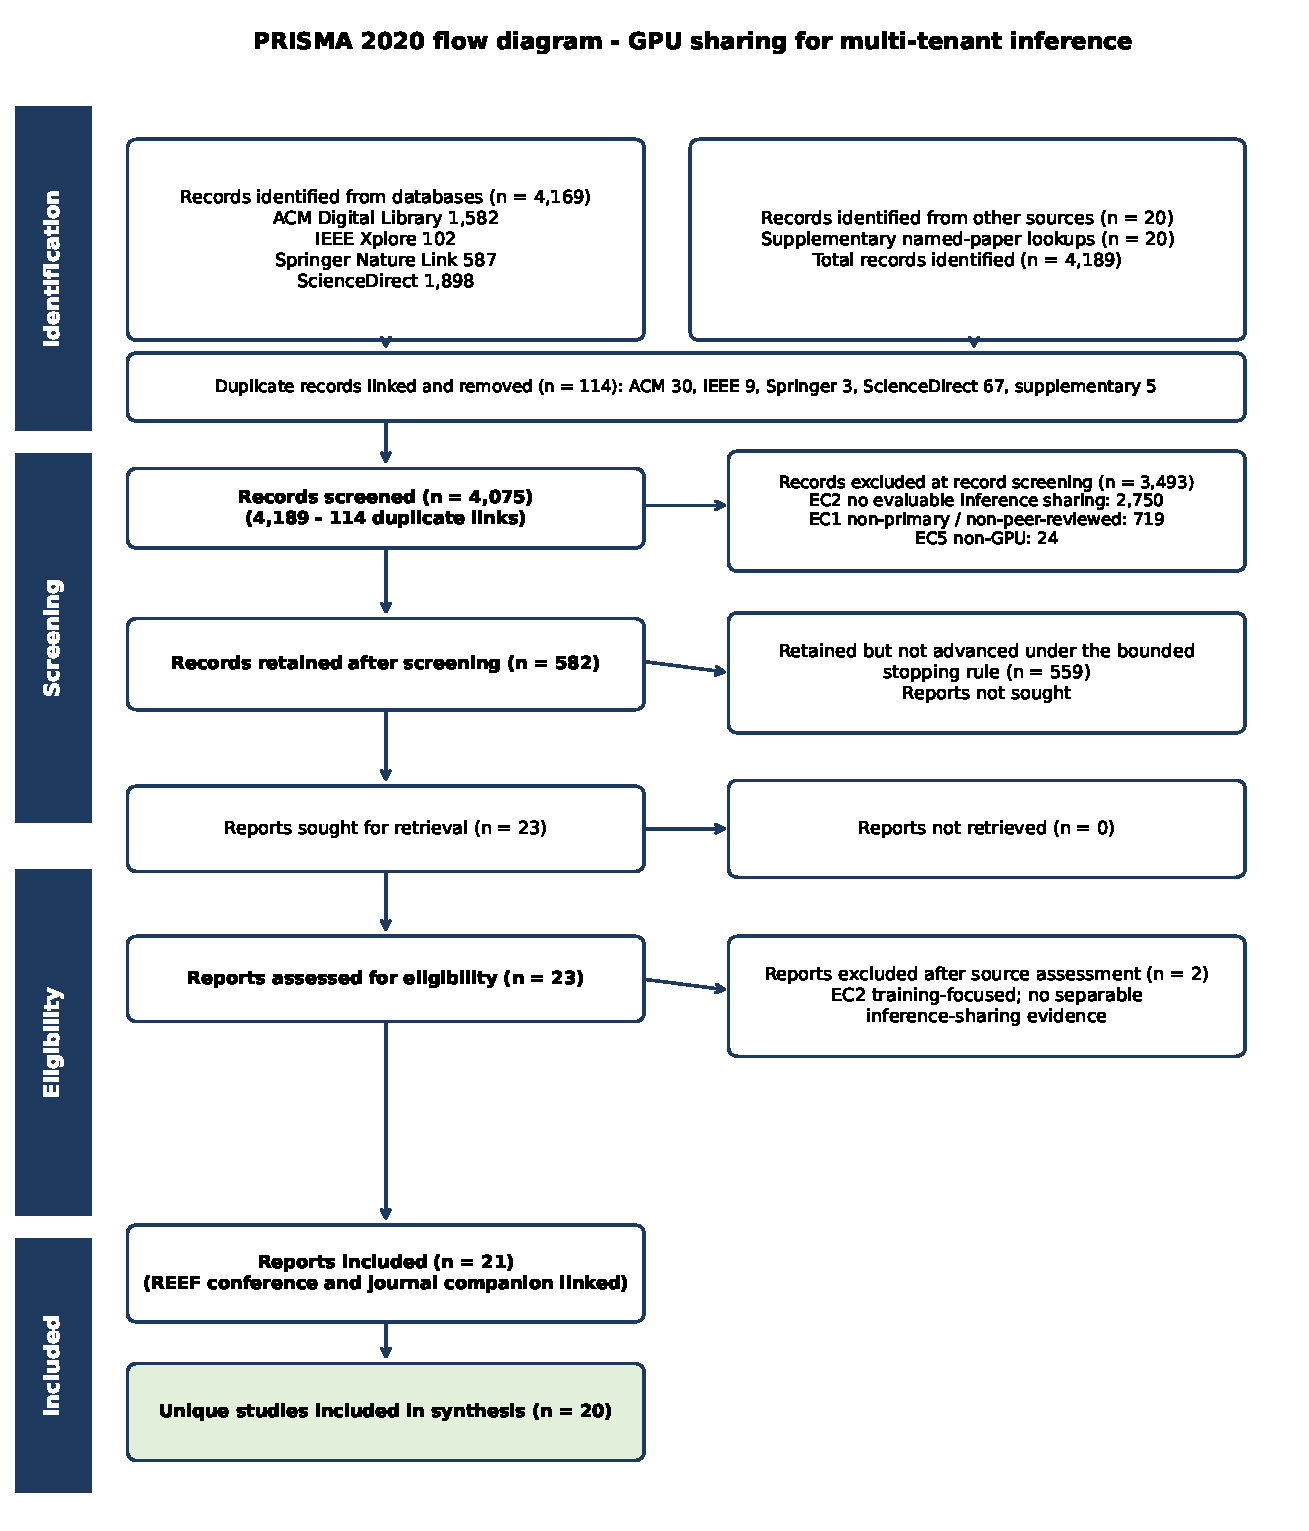
\includegraphics[width=\textwidth,height=.82\textheight,keepaspectratio]{figures/Frozen_PRISMA.pdf}
\caption{Frozen Task 2 selection flow, shown as historical provenance only. The adjacent branch table records later decisions; a reconciled final whole-review PRISMA flow remains pending.}
\end{figure}
\begin{longtable}{>{\raggedright\arraybackslash}p{0.16\textwidth}>{\raggedright\arraybackslash}p{0.62\textwidth}>{\raggedright\arraybackslash}p{0.1\textwidth}}
\toprule
\textbf{Study / report} & \textbf{System / source identity} & \textbf{QA}\\\midrule\endhead
S001 / P001 & VastPipe (2025) & 13/18\\\addlinespace
S002 / P002 & iGniter (2023) & 18/20\\\addlinespace
S003 / P003 & gpulets (2022) & 20/20\\\addlinespace
S004 / P004 & PipeSwitch (2020) & 17/20\\\addlinespace
S005 / P005 & REEF conference (2022) & 18/20\\\addlinespace
S006 / P006 & Paella: Low-latency Model Serving with Software-defined GPU Scheduling (2023) & 16/18\\\addlinespace
S007 / P007 & Orion: Interference-aware, Fine-grained GPU Sharing for ML Applications (2024) & 19/20\\\addlinespace
S008 / P008 & GSLICE: Controlled Spatial Sharing of GPUs for a Scalable Inference Platform (2020) & 17/20\\\addlinespace
S009 / P009 & Serving DNNs like Clockwork: Performance Predictability from the Bottom Up (2020) & 18/20\\\addlinespace
S010 / P010 & Colocating ML Inference and Training with Fast GPU Memory Handover (SIRIUS) (2025) & 17/20\\\addlinespace
S011 / P011 & ParvaGPU: Efficient Spatial GPU Sharing for Large-Scale DNN Inference in Cloud Environments (2024) & 14/20\\\addlinespace
S012 / P012 & Torpor: GPU-Enabled Serverless Computing for Low-Latency, Resource-Efficient Inference (2025) & 15/20\\\addlinespace
S013 / P013 & StreamBox: A Lightweight GPU SandBox for Serverless Inference Workflow (2024) & 17/20\\\addlinespace
S014 / P014 & Efficient Performance-Aware GPU Sharing with Compatibility and Isolation through Kernel Space Interception (KRYPTON) (2025) & 16/20\\\addlinespace
S015 / P015 & XSched: Preemptive Scheduling for Diverse XPUs (2025) & 18/20\\\addlinespace
S016 / P018 & InferFair: Towards QoS-aware scheduling for performance isolation guarantee in heterogeneous model serving systems (2024) & 17/20\\\addlinespace
S017 / P019 & ArkGPU: enabling applications' high-goodput co-location execution on multitasking GPUs (2023) & 16/20\\\addlinespace
S018 / P020 & Dyna-P: placement-aware dynamic partitioning for lightweight applications with modern GPUs (2025) & 15/20\\\addlinespace
S019 / P021 & KRISP: Enabling Kernel-wise RIght-sizing for Spatial Partitioned GPU Inference Servers (2023) & 18/20\\\addlinespace
S020 / P022 & Tally: Non-Intrusive Performance Isolation for Concurrent Deep Learning Workloads (2025) & 19/20\\\addlinespace
S021 / P024 & LithOS (2025) & 17/20\\\addlinespace
S022 / P025 & Abacus (2021) & 17/20\\\addlinespace
S023 / P026 & Miriam (2023) & 16/20\\\addlinespace
S024 / P027 & SGDRC (2025) & 16/20\\\addlinespace
S025 / P028 & Pantheon (2024) & 16/20\\\addlinespace
S026 / P029 & Oneiros (2025) & 17/20\\\addlinespace
S027 / P030 & GACER (2024) & 13/18\\\addlinespace
S028 / P031 & ElasticRoom (2024) & 15/20\\\addlinespace
S029 / P032 & SPLIT (2023) & 14/18\\\addlinespace
S030 / P033 & KACE (2024) & 14/16\\\addlinespace
\bottomrule\end{longtable}

\section{Taxonomy of existing approaches}
A useful taxonomy separates the resource being controlled from the software layer implementing the policy. The same system may appear in more than one category. A MIG-based system can also use MPS; an API interceptor can enforce temporal scheduling; and memory handover can support mixed-workload co-location. Treating these as mutually exclusive labels would hide the source of the observed behavior.

\subsection{Temporal and priority control}
Temporal mechanisms decide which work runs and when another tenant can make progress. PipeSwitch emphasizes switching and model state, Clockwork emphasizes predictable execution and admission, while REEF, Paella, Orion and XSched expose different scheduling/preemption boundaries. Their integration costs and latency meanings differ. PipeSwitch's additional switching-related latency is not interchangeable with XSched's foreground P99 ratio or Paella's reported P99 reduction \cite{P004,P005,P006,P007,P009,P015}.

LithOS extends temporal control with transparent kernel atomization and TPC allocation; Abacus makes operator overlap deterministic so a controller can predict concurrent-service latency. Miriam and Pantheon target edge inference, but at different intervention boundaries: elastic kernels versus chunk preemption combined with early-exit variants. They are not interchangeable implementations of the same scheduler \cite{s021,s022,s023,s025}.

\subsection{Spatial allocation and partitions}
MPS-based allocation and software right-sizing regulate concurrent access to execution resources. VastPipe, iGniter, gpulets and GSLICE provide different allocation, profiling and feedback approaches. KRISP contributes AMD-oriented kernel right-sizing evidence and should not be relabeled as a measurement of NVIDIA MPS. Partition-aware designs, including ParvaGPU and Dyna-P, additionally make placement, profile size or reconfiguration relevant \cite{P001,P002,P003,P008,P011,P020,P021}.

A spatial allocation is only one part of a service guarantee. The model must fit memory, the workload must remain within the profiled regime and the selected resource shares must satisfy its timing requirements. Hardware allocation boundaries do not by themselves establish all possible security or fault guarantees in the reviewed experiments.

\subsection{API, runtime and memory mediation}
Torpor, StreamBox, KRYPTON, ArkGPU and Tally intervene at different points between the application and accelerator. Their common advantage is control over resource use without necessarily changing the model's high-level purpose. Their differences include intercepted interfaces, compatibility, runtime sharing, host work and the degree to which tenants share memory or trust assumptions. SIRIUS contributes a specific memory-handover mechanism for co-located inference and training \cite{P010,P012,P013,P014,P019,P022}.
SGDRC dynamically controls compute and VRAM-bandwidth contention through software mechanisms, while Oneiros remaps model-parameter memory and overlaps CPU/GPU transfers to relieve multi-model memory pressure. Oneiros evaluates temporal and spatial configurations; its memory-management benefit is not a new fault-containment guarantee. SGDRC explicitly reports that its shared CUDA context cannot isolate DNN GPU-runtime failures \cite{s024,s026}.

\begin{longtable}{>{\raggedright\arraybackslash}p{0.25\textwidth}>{\raggedright\arraybackslash}p{0.35\textwidth}>{\raggedright\arraybackslash}p{0.28\textwidth}}
\toprule
\textbf{Family / reports} & \textbf{Control and condition} & \textbf{Cost}\\\midrule\endhead
Temporal / priority; P004 P005 P006 P007 P009 P015 P022 & Request, model, kernel or launch order. A suitable interception/preemption boundary exists & Switch cost, profiling and background slowdown\\\addlinespace
Software spatial sharing; P001 P002 P003 P008 P021 & MPS quota or AMD CU-mask control. Concurrent jobs fit memory and selected compute allocation & Residual interference; quotas are not proof of security\\\addlinespace
Hardware partition and hybrid; P011 P014 P020 & MIG profiles plus temporal/MPS policy. Supported partition profiles fit model memory & Fragmentation, placement and reconfiguration cost\\\addlinespace
API / runtime mediation; P006 P012 P013 P014 P019 P022 & User API, shared runtime or kernel interface. Required APIs and integration hooks are supported & Compatibility, CPU/transfer cost and trust boundary\\\addlinespace
Memory handover; P010 & Inference/training memory ownership. Training can yield memory without breaking inference & Reclamation and integration overhead\\\addlinespace
Fairness policy; P018 & Relative model slowdown and SLO goodput. Comparable per-model service objectives & Not equivalent to request-tail or hostile-tenant isolation\\\addlinespace
Fine-grained temporal / spatial control; P024 P025 P026 & TPC/atomization, deterministic operator overlap and elastic kernels; compatibility and profiled workload assumptions & Kernel support, profiling, latency versus throughput\\\addlinespace
Software compute/bandwidth control; P027 & SM allocation and software VRAM-bandwidth control; shared CUDA context & No DNN runtime-fault isolation\\\addlinespace
Model-adaptive edge preemption; P028 & Chunk preemption plus early-exit variants; permitted accuracy/memory budget & Deadline behavior changes both model work and scheduler cost\\\addlinespace
Parameter-memory virtualization; P029 & Temporal/spatial multi-model service with asynchronous transfer; high CPU/GPU bandwidth & Transfer overhead, memory policy and isolation claims separate\\\addlinespace
\bottomrule\end{longtable}\paragraph{Two further software boundaries.} ElasticRoom coordinates resource-constrained compilation and runtime priorities, while SPLIT uses model-block temporal preemption over independently arriving tasks. Neither is a new hardware partition; sequential execution in SPLIT remains GPU sharing through time multiplexing \cite{s028,s029}.

\paragraph{Kernel-aware MPS colocation.} KACE selects a sharing partner using offline kernel and system metrics. Its single-V100 experiment separately identifies inference targets, including ViT, BERT and speech models. The ViT batch-2 example shows why a small-memory BERT inference partner can still cause compute contention. Its outcome is oracle-normalized pair throughput, not request-tail latency. Aggregate gains over mixed training/inference targets are retained as context rather than inference-only effects. KACE is not uniformly best: the adapted Xu policy and MEMCAP win six and two of the 21 mixed-mode cases respectively. This supports profiling-aware partner selection for throughput-oriented services, with separate latency and protection validation when those are required \cite{s030}.
\paragraph{Cross-stack extension.} GACER belongs to compiler/runtime coordination: spatial microbatch splitting and temporal cross-model scheduling complement native streams. This resource-efficiency control does not assert a fault/security boundary \cite{s027}.


\section{Results and evidence synthesis by research question}
\subsection{RQ1: mechanisms and control boundaries}
The corpus supports a layered answer rather than a product list. Temporal control manages ordering and interruption; software spatial control manages concurrent allocation; hardware partitioning constrains resource placement; and API/runtime mediation supplies an enforcement layer. Fairness-aware policy adds a decision objective across these mechanisms. InferFair, for example, is best understood through relative slowdown and useful service, not as a new hardware partition primitive \cite{P018}.

This taxonomy explains why naming MPS, MIG or remoting is insufficient for engineering selection. A deployment also needs a policy, a mechanism for enforcing it and an explicit boundary of protection. The corpus demonstrates several combinations, but its bounded selection does not support a claim that one category is most prevalent in the entire literature.

The 10 additions reinforce the layered taxonomy. LithOS coordinates TPC scheduling and atomization, Abacus coordinates operator overlap, Miriam transforms kernels, Pantheon combines chunk preemption with model adaptation, SGDRC controls compute and memory bandwidth, and Oneiros controls parameter-memory residency. The enforcement point and shared state explain which mechanisms can be composed and which integration assumptions must be checked \cite{s021,s022,s023,s024,s025,s026}.

Compiler/runtime approaches also differ internally. ElasticRoom generates resource-constrained kernel candidates and applies priority-aware runtime ordering; GACER uses microbatch and operator coordination. SPLIT instead schedules requests sequentially at model-block boundaries. These are software controls over different resources, not interchangeable MIG-like partitions \cite{s027,s028,s029}.

\subsection{RQ2: measurements and comparability}
The outcome register includes requests/s, normalized throughput, goodput, P99/P98 latency, unspecified latency, SLO-violation rate, API overhead, host memory and a composite utilization-efficacy score. These measure different properties. Goodput counts work that meets a service objective, while aggregate throughput may include best-effort work that does not protect the foreground service. A numerical increase in the latter cannot establish improvement in the former.

GSLICE's GUE value of 94.04 is a composite score, not 94.04\% GPU utilization. Its negative signed latency improvement is retained as an unfavorable observation. The gpulets threshold covering 90\% of tested model pairs concerns a distribution across pairs, not the 90th percentile of requests. These distinctions prevent apparently precise but invalid conclusions \cite{P003,P008}.

The reported iGniter prediction-error range of 1.53--5.02\% assesses prediction accuracy, not a latency speedup. Clockwork's approximately 800 requests/s is goodput in a particular evaluation, and the supplied extraction notes a nonidentical comparator setup. Both observations are useful, but neither supports a direct ranking against a throughput ratio measured on another platform \cite{P002,P009}.

Pantheon's deadline-adjusted relative accuracy treats a late job as zero accuracy; it is not ordinary classification accuracy. Abacus excludes deadline-dropped queries from latency calculations while including them in QoS violations, so latency must be read with the violation population. Oneiros separates P99 time-to-first-token (TTFT), including queuing, from time-between-token (TBT), and reports throughput in generated tokens/s. None is directly interchangeable with DNN requests/s or an unspecified latency statistic \cite{s022,s025,s026}.

ElasticRoom's Goodput divides QoS-satisfying requests by maximum batch inference latency, and its main real-time endpoint is mean end-to-end latency including queuing. SPLIT measures target-relative violation fraction and calls block-execution-time dispersion jitter. These definitions differ from GACER's batch completion and Oneiros's P99 token latencies; no numeric cross-study average is justified \cite{s027,s028,s029,s026}.

\subsection{RQ3: conditions affecting results}
Three conditions recur in the evidence. First, concurrency and resource shares affect both completed work and waiting time. The local ParvaGPU contrast shows a throughput benefit accompanied by increased latency. Second, model state and memory transfer can dominate. Torpor's late binding is attractive for low-rate functions, but its density result does not establish that frequent transfers of large models meet the same latency objective. Third, the workload's priority structure determines which sacrifice is acceptable \cite{P011,P012}.

For a foreground-priority service, XSched's 1.07x standalone P99 is relevant because it directly expresses foreground interference in the evaluated setup. Orion's up-to-7.3x aggregate-throughput result describes total work and must be read with its foreground-latency condition. These results can support different decisions without contradicting each other \cite{P007,P015}.

Mixed-workload evidence requires an additional separation. SIRIUS reports an average P99 inference improvement factor of 12.6 against the authors' adapted TaskSwitch baseline. It is not a uniform per-model gain or a direct comparison against unmodified PipeSwitch. ArkGPU's recorded inference/training pairs meet a twice-solo P99 target, while a low-contention setting can lose about 5\% QPS. The unfavorable condition belongs in the synthesis because it changes when the mechanism is worthwhile \cite{P010,P019}.

Miriam's RTX2060 and edge-device results differ by workload and arrival mode; the introductory latency-overhead summary is not a universal bound for the body experiments. Pantheon reports 0.39--1.10\% deadline misses for three stated application mixes, but does so with model-variant, memory and accuracy constraints. Oneiros's C1 spatial-sharing comparison reports author-averaged reductions of 65.5\% in P99 TBT and 20.7\% in P99 TTFT, with 6.6\% higher tokens/s, under the stated trace and model mix. These are within-source conditions, not transferable service guarantees \cite{s023,s025,s026}.

On A100, ElasticRoom reports 22\% lower mean real-time latency and 1.43 times its defined Goodput relative to its described REEF policy. On MI100, its specified Conv2/Conv3 candidates can perform worse than Ansor by less than 8\%, and sustained execution drift can undermine offline choices. SPLIT's ResNet50 splitting overhead rises from 15.4\% for two blocks to 50.3\% for four. Its short-request stability gain can sacrifice long-request stability. More variants or finer splitting therefore do not uniformly improve service \cite{s028,s029}.

\subsection{RQ4: isolation and implementation cost}
Performance isolation asks whether another workload changes service behavior. Resource isolation asks what capacity is allocated or separated. Memory protection and fault containment concern different failure or adversarial models. A scheduler that limits slowdown is not thereby a complete hostile-tenant security boundary. The extraction cards preserve these dimensions separately, and untested boundaries remain unestablished.

Implementation costs also operate at different levels. API mediation can add host-side work or per-call delay. Model swapping adds transfer and memory pressure. Kernel-space interception introduces compatibility and maintenance requirements. Temporal granularity changes the trade-off between scheduling work and waiting time. The KRYPTON extraction reports an average QoS violation rate of 1.23\% relative to a solo P99 threshold, which is a threshold-relative request fraction rather than a latency in milliseconds. Its original Poisson rate is half the solo maximum; the shared test halves that rate again while assigning 50\% time \cite{P014}.

SGDRC's shared-context execution provides performance control without DNN runtime-fault isolation. Pantheon prioritizes deadlines by trading some model accuracy and memory residency for schedulability, and adds device power relative to its comparator. Abacus incurs profiling and predictor work. LithOS requires compatible interception and kernel behavior; Oneiros relies on high CPU/GPU transfer bandwidth and must cap remapping to avoid extra latency. These costs should be compared to the deployment's constraint, not collapsed into a single isolation or overhead score \cite{s021,s022,s024,s025,s026}.

ElasticRoom's virtual-room abstraction concerns performance coordination; it does not demonstrate fault containment. SPLIT's token-controlled sequential execution avoids simultaneous-kernel contention, but does not establish adversarial or runtime-fault separation. Both require model knowledge and offline work, with missing configuration and repeated-trial details limiting transfer. Isolation requirements must be specified separately from the reported QoS benefit \cite{s028,s029}.

\subsection{RQ5: conditional selection}
The evidence supports a sequence of decisions. Specify the service objective and trust boundary first. Eliminate mechanisms incompatible with hardware, model memory or required integration. Compare the remaining candidates under the relevant arrival process, batch and co-tenant mix. Measure both protected service and work sacrificed. If the available studies do not cover the required boundary, the appropriate conclusion is insufficient evidence for that guarantee, not an assumed benefit.

The recommendation matrix in Section~10 connects each scenario to report IDs, expected benefits, costs and alternatives. These are evidence-supported candidates for evaluation, not claims that the reviewed implementation can be deployed unchanged in every environment.

The added evidence broadens the candidate set without changing the selection rule. For predictable co-located DNN service, deterministic overlap or fine-grained priority control is a candidate when profiling and compatible kernels are acceptable. For an edge deadline objective, model-changing approaches require an explicit accuracy budget. For memory-constrained multi-LLM service on a high-bandwidth CPU/GPU system, parameter remapping is a candidate while transfer cost remains tolerable. Fault-sensitive or mutually untrusted tenants require a separately established boundary \cite{s021,s022,s023,s024,s025,s026}.

A compiler/runtime candidate is appropriate when the workload and toolchain permit variant generation and priority control. A block-preemptive temporal candidate is appropriate when static model graphs and splitting costs fit the service budget. Choose neither merely because its headline percentage is larger: ElasticRoom changes resource-constrained kernels, while SPLIT changes model execution boundaries, and their endpoints are not matched \cite{s028,s029}.

\section{Comparative analysis}
The comparison distinguishes direct within-source contrasts from unmatched cross-study observations. The strongest numerical statements are tied to their original comparator. Even these require attention to whether the result is an average, maximum, lower bound or threshold-relative statistic. An improvement described as ``up to'' is not the expected result for an arbitrary deployment.

\begin{longtable}{>{\raggedright\arraybackslash}p{0.26\textwidth}>{\raggedright\arraybackslash}p{0.28\textwidth}>{\raggedright\arraybackslash}p{0.34\textwidth}}
\toprule
\textbf{Evidence / class} & \textbf{Observation} & \textbf{Interpretation and missing control}\\\midrule\endhead
CMP01 P011 E036 E037 C001 C002. Within-source trade-off & 354 to 446 requests/s; 11 to 27 ms & 25.99\% throughput increase accompanies 2.4545x latency. Missing: Latency quantile; final version equivalence\\\addlinespace
CMP02 P001 E001; P011 E036. Unmatched cross-study & 2.7x versus 25.99\% increase & Different baseline and GPU/model context prevent ranking. Missing: Matched workload, batch and resource budget\\\addlinespace
CMP03 P007 E029 E030; P015 E044. Different objectives & Up to 7.3x aggregate work versus 1.07x foreground P99 & Foreground delay and total completed work must be assessed together. Missing: Common model mix and background progress metric\\\addlinespace
CMP04 P008 E031 E032. Within-source metric tension & GUE 94.04 and negative signed latency improvement & Composite efficacy is not utilization percent; preserve adverse latency. Missing: Metric definitions and baseline stratum\\\addlinespace
CMP05 P012 E038 E039. Condition-dependent trade-off & Density benefit with model-transfer sensitivity & Late binding suits low-rate functions only if transfer fits SLO. Missing: Heavy-model transfer and host CPU budget\\\addlinespace
CMP06 P019 E048 E049; P022 E052. Different experiments, consistent cost & ArkGPU approximately 5\%low-contention QPS regression; Tally total normalized throughput1.19 versusTGS1.65 & Foreground protection can carry aggregate or co-tenant costs; Tally outcome is total system throughput.. Missing: Matched slowdown definitions\\\addlinespace
CMP07 P005 P023. Companion study, not replication & REEF engines and report versions differ & Retain source-version strata; do not double-count corroboration. Missing: No current combined numerical rows: E018-E026 explicitly assigned to conferenceP005; journal experiments remain separate.\\\addlinespace
CMP08 P018 E046 E047; P020 E050. Different metrics & Goodput/fairness versus makespan & Job-level efficiency cannot establish request-tail service. Missing: Request arrival process and latency distribution\\\addlinespace
CMP09 P024 / LITH-01--02. Within-source tenant-set limitation & LithOS SLO attainment100\%; normalized throughput1.0 versus MPS1.11 in the logged scenario & MIG/Limits omit BE while LithOS/MPS include it; no matched all-family ranking\\\addlinespace
CMP10 P025 / ABAC rows. Population distinction & p99 improvement and peak query throughput use distinct load/settings & Deadline-dropped queries excluded from latency but counted in violations\\\addlinespace
CMP11 P026 P028. Unmatched edge experiments & Elastic kernels versus model-variant/chunk preemption & Different models, platforms and accuracy semantics; not a direct winner comparison\\\addlinespace
CMP12 P027 / SGDRC rows. Goodput versus raw throughput & Latency-sensitive protection with BE progress; adverse raw throughput retained & Shared context lacks runtime-fault isolation; baseline reimplementation matters\\\addlinespace
CMP13 P029 / ONEI-01--03. Within-source spatial case & 65.5\% lower P99 TBT; 20.7\% lower P99 TTFT; 6.6\% higher tokens/s & C1 model mix and traces; source averages, not a general hardware effect\\\addlinespace
CMP14 P031 / ELAST-01--02. Defined endpoint & 22\% lower mean RT latency;1.43times source-defined Goodput against described REEF policy & A100;batch1; source averages; mean latency is notp99; adapted comparator/scenario ambiguities retained\\\addlinespace
CMP15 P032 / SPLIT-04--05. Adverse split configuration & ResNet50 two-block overhead15.4\%;four-block50.3\% & Additional sum-of-block execution cost versus vanilla model; blockSDjitter differs from request-tail latency\\\addlinespace
\bottomrule\end{longtable}
\paragraph{Kernel-aware MPS colocation.} KACE selects a sharing partner using offline kernel and system metrics. Its single-V100 experiment separately identifies inference targets, including ViT, BERT and speech models. The ViT batch-2 example shows why a small-memory BERT inference partner can still cause compute contention. Its outcome is oracle-normalized pair throughput, not request-tail latency. Aggregate gains over mixed training/inference targets are retained as context rather than inference-only effects. KACE is not uniformly best: the adapted Xu policy and MEMCAP win six and two of the 21 mixed-mode cases respectively. This supports profiling-aware partner selection for throughput-oriented services, with separate latency and protection validation when those are required \cite{s030}.
\subsection{Compiler/runtime coordination and batch-latency evidence}
GACER extends the fine-grained compiler/runtime family through microbatch splitting and staged cross-model operator scheduling over GPU streams. Its final ICCAD2024 report evaluates heterogeneous inference models on one A100 and separately on P6000 and GTX1080Ti devices. Table2 reports3.30ms for VGG16+LSTM versus4.32ms sequential and22.14ms for five models versus37.86ms sequential. These are batch-completion measurements, not per-request tail latencies or online SLO attainment. Achieved SM occupancy is likewise distinct from GPU busy-time utilization. Table3 reports0.84--1.26seconds of optimization across the stated mixes and batches. This supports a conditional choice for known multi-model batch workloads when optimization and transformation costs are tolerable; it does not establish fault isolation or superiority on online tail-SLO objectives. The final report has four authors and nine pages, differing from the older seven-author preprint, which does not supply the extracted final results \cite{s027}.


The evidence tables in Appendices~\ref{app:evidence} and \ref{app:additions} retain 52 inherited and 38 new observations, respectively. The comparative matrix is deliberately smaller because its role is to explain a decision, not duplicate the extraction register. A claim can be traced from a recommendation to a report, then to an outcome ID and its page/figure anchor. Where a comparison remains unmatched, the matrix names the missing control rather than calculating a misleading combined effect.

\section{Engineering trade-off analysis}
\subsection{Utilization versus latency}
Additional concurrency is beneficial only while useful service increases under the required latency objective. The ParvaGPU example changes throughput by
\[ (446/354-1)\times100 = 25.99\%, \]
while latency changes by
\[ 27/11 = 2.4545. \]
These are calculations from recorded inputs, not newly measured outcomes. A service with a tight delay budget might reject this configuration despite its higher throughput. Another service might accept it if the increased latency remains within its own budget. Because the source quantile is unspecified, neither interpretation establishes P99 compliance \cite{P011}.

\subsection{Foreground protection versus background progress}
Priority is an allocation choice. Tally's supplied contrast records normalized total system throughput of 1.19 versus 1.65 for TGS at the 10\% idle-time setting. This does not make foreground protection ineffective; it identifies the work sacrificed. Similarly, an aggregate-throughput gain must not hide deterioration in the protected request class. The engineering evaluation should report foreground latency and background progress together \cite{P022}.

\subsection{Memory density versus transfer and trust costs}
Shared runtimes and late binding can allow more functions or models to use limited GPU memory. StreamBox's workflow-oriented sharing and Torpor's binding decisions address this problem from different directions. Their density gains cannot be separated from concurrency, model-loading and trust assumptions. When large models are invoked frequently, transfer demand can undermine the benefit of keeping fewer models resident. When functions require stronger separation, a shared runtime may not provide the required boundary. Torpor explicitly distinguishes runtime-sharing evaluation from runtime-isolation deployment, and describes restart/migration recovery; these design claims are not direct fault-injection results \cite{P012,P013}.

\subsection{Deadlines versus model accuracy and memory}
Pantheon gives a different trade-off from a scheduler that preserves the original model unchanged: its early-exit variants reduce work when needed to protect deadlines. The reported deadline-adjusted accuracy therefore couples model quality and timeliness. Its similar utilization to RTm-DL does not establish universal utilization superiority. Miriam likewise requires workload-specific reading of throughput and critical-task latency rather than importing its introductory summary as a hard bound \cite{s023,s025}.

\subsection{Memory capacity versus transfer bandwidth}
Oneiros trades parameter residency for KV-cache capacity and asynchronous transfer. Its spatial-sharing gains occur in a stated GH200 setup and model mix; more aggressive remapping can increase average latency, and halting remapping at low load can help. This complements, rather than directly supersedes, Torpor's low-rate late-binding evidence because model scale, transfer path and metrics differ \cite{P012,s026}.

\subsection{Partition control versus flexibility}
Hardware profiles constrain placement and memory fit. Software policies can improve use of a chosen profile, but fine-grained application demand need not align with fixed partitions. Dyna-P's recorded sensitivity to prediction perturbation concerns makespan, while online serving additionally needs evidence about individual request delays. The review therefore treats placement efficiency as relevant but insufficient evidence for latency-sensitive request serving \cite{P020}.

\section{Discussion and conflicting evidence}
\subsection{Apparent conflicts versus controlled disagreements}
A valid conflicting-evidence analysis first asks whether two studies measure the same quantity under comparable conditions. VastPipe's 2.7x throughput contrast and the calculated 25.99\% ParvaGPU increase have different baselines and workloads. Their unequal magnitudes do not show disagreement. Likewise, Orion's aggregate throughput, SIRIUS's average P99 improvement and XSched's normalized foreground P99 do not compete on a common scale \cite{P001,P007,P010,P011,P015}.

More useful tensions occur inside an experiment: improved throughput accompanied by higher latency, or protection of foreground work accompanied by lower background progress. The negative GSLICE latency contrast and ArkGPU's low-contention regression show conditions in which a favorable overall mechanism narrative is incomplete. These observations constrain applicability rather than being dismissed as exceptions \cite{P008,P019}.

The added papers supply further within-source tensions. LithOS's plotted SLO advantage must be read with an unequal supported tenant set for some comparators. SGDRC can trade raw aggregate throughput for latency-sensitive goodput; it does not dominate every throughput baseline. Pantheon's lower deadline-miss rate coexists with model/memory changes, and its power experiment reports 10.15 W versus RTm-DL's 9.73 W. These are conditional costs, not mutually contradictory claims across unmatched systems \cite{s021,s024,s025}.

Baseline adaptation is material in the new evidence. ElasticRoom's KRISP comparator uses ElasticRoom-generated kernels and REEF-like priority, so it is not an unchanged original KRISP experiment. SPLIT's abstract calls its 43\% headline a violation-rate reduction, whereas its conclusion calls it a response-ratio reduction; the two endpoints are not silently equated. The extraction excludes that ambiguous headline from the quantitative synthesis and preserves the directly specified alternatives \cite{s028,s029}.

\subsection{Version and engine effects}
The REEF journal extension adds implementation and evaluation beyond the conference report. The supplied extraction already distinguishes PyTorch and TensorRT conditions in its discussion. Combining all favorable points into one synthetic result would obscure both the engine difference and the report-version difference. All nine retained REEF rows E018--E026 are now explicitly assigned to the conference P005 and its AMD evaluation stratum. P023 supplies companion context; its expanded NVIDIA and LLM experiments are separate and are not transplanted into those rows \cite{P005,P023}.

\subsection{Strength of the engineering argument}
The repeated pattern is that resource sharing works through a mechanism-specific constraint: interruption cost, quota fit, memory residency, partition placement or compatibility. This pattern supports conditional design reasoning. It does not establish identical effect sizes or a common security guarantee across systems. The draft's recommendations remain narrower than a claim of deployment readiness.

\section{Evidence-based engineering recommendations}
\subsubsection*{REC01: Trusted resident models; utilization priority}
\begin{longtable}{>{\raggedright\arraybackslash}p{0.22\textwidth}>{\raggedright\arraybackslash}p{0.7\textwidth}}
\toprule
\textbf{Dimension} & \textbf{Assessment}\\\midrule\endhead
Candidate & Tuned MPS / software spatial controls\\\addlinespace
Evidence & P001 P002 P003 P008 E001-E004 E006 E031-E032\\\addlinespace
Expected benefit & Higher useful co-location under tested allocations\\\addlinespace
Sacrifice & Interference, quota tuning and memory pressure\\\addlinespace
Alternative / trigger & Partitions or dedication when trust/isolation dominates\\\addlinespace
Validation needed & Measure each model P99 and SLO goodput under bursts\\\addlinespace
\bottomrule\end{longtable}
\subsubsection*{REC02: Foreground tail-latency priority}
\begin{longtable}{>{\raggedright\arraybackslash}p{0.22\textwidth}>{\raggedright\arraybackslash}p{0.7\textwidth}}
\toprule
\textbf{Dimension} & \textbf{Assessment}\\\midrule\endhead
Candidate & Priority/preemptive scheduling\\\addlinespace
Evidence & P005 P006 P007 P015 P022 E018-E030 E044-E045 E052\\\addlinespace
Expected benefit & Lower foreground interference\\\addlinespace
Sacrifice & Background slowdown, profiling and runtime integration\\\addlinespace
Alternative / trigger & Dedicated GPU when supported control cannot meet deadline\\\addlinespace
Validation needed & Check foreground tails and background progress jointly\\\addlinespace
\bottomrule\end{longtable}
\subsubsection*{REC03: Low-rate serverless functions}
\begin{longtable}{>{\raggedright\arraybackslash}p{0.22\textwidth}>{\raggedright\arraybackslash}p{0.7\textwidth}}
\toprule
\textbf{Dimension} & \textbf{Assessment}\\\midrule\endhead
Candidate & Late binding / controlled runtime sharing\\\addlinespace
Evidence & P012 P013 E038-E041\\\addlinespace
Expected benefit & Higher function or workflow density\\\addlinespace
Sacrifice & Host CPU, memory transfer and shared-runtime trust\\\addlinespace
Alternative / trigger & Keep large or high-rate models resident if swaps dominate\\\addlinespace
Validation needed & Sweep model sizes, cold starts, offered rate and concurrency\\\addlinespace
\bottomrule\end{longtable}
\subsubsection*{REC04: Mixed inference with opportunistic training}
\begin{longtable}{>{\raggedright\arraybackslash}p{0.22\textwidth}>{\raggedright\arraybackslash}p{0.7\textwidth}}
\toprule
\textbf{Dimension} & \textbf{Assessment}\\\midrule\endhead
Candidate & Memory handover / controlled co-location\\\addlinespace
Evidence & P010 P019 E035 E048-E049\\\addlinespace
Expected benefit & Protect inference while using residual capacity\\\addlinespace
Sacrifice & Memory/reclamation costs and possible co-tenant regression; ArkGPU approximately 5\%QPS loss under low contention.\\\addlinespace
Alternative / trigger & Separate resources for intolerable interference\\\addlinespace
Validation needed & Measure inference tails separately from training throughput\\\addlinespace
\bottomrule\end{longtable}
\subsubsection*{REC05: Supported partition hardware; stable memory fit}
\begin{longtable}{>{\raggedright\arraybackslash}p{0.22\textwidth}>{\raggedright\arraybackslash}p{0.7\textwidth}}
\toprule
\textbf{Dimension} & \textbf{Assessment}\\\midrule\endhead
Candidate & MIG-aware hybrid policy\\\addlinespace
Evidence & P011 P014 P020 E036-E037 E042-E043 E050\\\addlinespace
Expected benefit & Resource allocation with configurable co-location\\\addlinespace
Sacrifice & Fragmentation and reconfiguration overhead\\\addlinespace
Alternative / trigger & Software sharing when partition granularity wastes capacity\\\addlinespace
Validation needed & Validate profile fit and online request tails; Dyna-P8.09\%makespan penalty at15\%prediction perturbation is local, not Section4.3.2simulation.\\\addlinespace
\bottomrule\end{longtable}
\subsubsection*{REC06: Several models with unequal service pressure}
\begin{longtable}{>{\raggedright\arraybackslash}p{0.22\textwidth}>{\raggedright\arraybackslash}p{0.7\textwidth}}
\toprule
\textbf{Dimension} & \textbf{Assessment}\\\midrule\endhead
Candidate & Fairness-aware admission / scheduling\\\addlinespace
Evidence & P018 E046-E047\\\addlinespace
Expected benefit & In \nolinkurl{Table3ratio3:1:2,total600requests/s:} goodput524.29 versusClockwork457.24; unfairness1.05 versus1.50.\\\addlinespace
Sacrifice & May give up aggregate throughput to improve fairness\\\addlinespace
Alternative / trigger & Priority scheduling when one foreground SLA dominates\\\addlinespace
Validation needed & Validate intended SLO/arrival mix; source uses100msSLO,50msperiod and max/min slowdown unfairness. No universal throughput advantage is inferred.\\\addlinespace
\bottomrule\end{longtable}
\subsubsection*{REC07: Predictable multi-model DNN co-location}
Abacus and LithOS broaden the candidate set where deterministic overlap or fine-grained resource control is compatible with the workload. Evaluate inference-only results separately from mixed training, preserve co-tenant sets, and measure profiling, host and kernel-support costs. Use a more conservative allocation when the protected service cannot tolerate the measured tail or unsupported kernels \cite{s021,s022}.

\subsubsection*{REC08: Edge deadlines with an explicit accuracy budget}
Consider Miriam for elastic-kernel coordination and Pantheon when chunk preemption and early-exit model variants are acceptable. The expected benefit is lower deadline interference under the evaluated mix; the sacrifice can include altered accuracy, extra resident variants, scheduling work and power. Prefer a model-preserving alternative when early exits violate task-quality requirements. Test nonperiodic arrivals, background progress and the actual platform rather than importing a single reported percentage \cite{s023,s025}.

\subsubsection*{REC09: Compute/bandwidth contention under a shared trust context}
SGDRC is a candidate for controlling compute and VRAM-bandwidth contention when its generated-kernel environment and shared CUDA context are acceptable. The expected benefit is latency-sensitive goodput with best-effort progress. It cannot be selected as a DNN runtime-fault boundary: that isolation is explicitly absent. Preserve cases where another baseline has greater raw throughput \cite{s024}.

\subsubsection*{REC10: Memory-constrained multi-LLM serving}
Oneiros is a candidate when a high-bandwidth CPU/GPU transfer path makes parameter remapping feasible. Its stated spatial-sharing case reports lower P99TBT/TTFT and higher tokens/s than vLLM. The sacrifice is transfer and remapping overhead; aggressive remapping can worsen average delay. Retain resident parameters or reduce remapping at low load or when transfers dominate, and establish required protection separately \cite{s026}.
\subsubsection*{REC11: Priority-aware CNN/BERT co-location with compilation access}
Consider ElasticRoom when generating kernel variants and maintaining offline tuning is feasible. Expect context-dependent real-time latency/Goodput improvement, while retaining model-specific no-gain cases, hardware drift and adverse generated kernels. Prefer a simpler or separately isolated mechanism when variant maintenance or a fault boundary is decisive \cite{s028}.
\subsubsection*{REC12: Static-DAG edge requests with mixed execution lengths}
Consider SPLIT when block-boundary preemption and its measured execution overhead fit the request budget. Short-request QoS can improve at the cost of long-request stability and spatial parallelism. Do not use the studied offline splitting method as evidence for input-dependent RNNs, arbitrary burst overload or universally reduced request-tail jitter \cite{s029}.

\paragraph{Kernel-aware MPS colocation.} KACE selects a sharing partner using offline kernel and system metrics. Its single-V100 experiment separately identifies inference targets, including ViT, BERT and speech models. The ViT batch-2 example shows why a small-memory BERT inference partner can still cause compute contention. Its outcome is oracle-normalized pair throughput, not request-tail latency. Aggregate gains over mixed training/inference targets are retained as context rather than inference-only effects. KACE is not uniformly best: the adapted Xu policy and MEMCAP win six and two of the 21 mixed-mode cases respectively. This supports profiling-aware partner selection for throughput-oriented services, with separate latency and protection validation when those are required \cite{s030}.
\paragraph{Known heterogeneous batch mixes.} Consider GACER when batch-completion efficiency is the objective and profiling/optimization delay is acceptable. Its reported 0.84--1.26 second optimization cost and absent serving-tail/fault evidence limit transfer to online SLO-sensitive or mutually untrusted tenants \cite{s027}.

The recommended deployment assessment begins with the actual service objective: per-model deadline or percentile target, admissible violation rate and minimum background progress. These values must come from the intended deployment rather than being invented from a paper. The next step is a local comparison using the same model versions, input sizes, batching and offered load. Cold starts and bursts should be retained if they occur in the application.

A candidate is suitable only if it meets the required service objective at an acceptable cost. The acceptance evidence should include per-tenant latency, SLO-compliant goodput, memory pressure, resource utilization with a defined instrument, host overhead and the relevant isolation tests. The review supplies a shortlist and the reasons to test it; it does not supply a universal numerical threshold or imply that a benchmark result transfers unchanged.

\section{Research gaps and future directions}
\begin{longtable}{>{\raggedright\arraybackslash}p{0.28\textwidth}>{\raggedright\arraybackslash}p{0.22\textwidth}>{\raggedright\arraybackslash}p{0.38\textwidth}}
\toprule
\textbf{Corpus gap} & \textbf{Basis} & \textbf{Next experiment}\\\midrule\endhead
No matched all-family comparison & Comparability CMP01-CMP08 & Same GPU, model mix, memory budget, arrivals and SLO across families\\\addlinespace
Security/fault boundaries often unestablished & Extraction Security boundary / Fault boundary & Separate adversarial access, fault injection and performance tests\\\addlinespace
Metrics emphasize different units & E001-E052 & Report per-model goodput, tails and background progress jointly\\\addlinespace
Partition prediction affects makespan & P020 E050 & Bursty arrivals plus placement changes and request-tail measurement\\\addlinespace
Version and method details remain incomplete & ParvaGPU final-text equivalence; source Q3/Q4/Q10 reporting limits. iGniter final checked; Tallyv3 pinned. & Publish exact version, driver/runtime, warmup, repetitions and uncertainty\\\addlinespace
Energy and cost evidence not harmonized & Extraction schema and heterogeneous outcomes & Measure GPU and host energy per SLO-compliant request\\\addlinespace
Model-adaptive versus model-preserving schedules & P028 changes exit/variant; P026 transforms kernels & Hold accuracy budget and input distribution constant; jointly report deadline and task quality\\\addlinespace
Multi-model memory remapping and protection & P029 capacity/latency results; no fault guarantee & Measure transfer, tenant progress, tail latency and fault behavior with explicit isolation boundaries\\\addlinespace
Source configuration/report inconsistencies & P025 A100 SM label; P026 platform label; P029 platform/isolation caption & Publish exact device identifiers and corrected experiment manifests\\\addlinespace
Compiler/kernel choice under hardware drift & ElasticRoom MI100 slowdown and adverse candidate cases & Evaluate refreshed profiles, matched baseline ports and repeatability under sustained runs\\\addlinespace
Block dispersion versus request stability & SPLIT uses blockSDjitter; short/long-task trade-off & Report actual request-latency distributions and per-task deadline outcomes jointly\\\addlinespace
\bottomrule\end{longtable}\paragraph{Throughput-oriented colocation and serving guarantees.} KACE identifies useful kernel features and inference-target contention, but does not establish request-level tail or fault isolation. Evaluate candidate-selection policies with identical arrival traces, per-tenant goodput, latency distributions and explicit protection requirements across GPU generations \cite{s030}.

These gaps are observations about this corpus and its reporting, not assertions that no relevant research exists anywhere. The 320 unresolved advanced records make that distinction essential. A stronger future comparison would align hardware, workload, baselines and outcome definitions across mechanism families, then report both benefits and sacrifices. Energy per useful request and failure/security behavior require separate measurements rather than extrapolation from utilization.

\section{Threats to validity and limitations}
\begin{longtable}{>{\raggedright\arraybackslash}p{0.32\textwidth}>{\raggedright\arraybackslash}p{0.26\textwidth}>{\raggedright\arraybackslash}p{0.3\textwidth}}
\toprule
\textbf{Threat / consequence} & \textbf{Mitigation} & \textbf{Remaining work}\\\midrule\endhead
Incomplete eligibility: No exhaustive recall or prevalence claim & 559screening decisions preserved;56borderline proposals reopened & Close320advanced records and report identities; reconcile whole-review flow\\\addlinespace
Title-only decisions: Relevant work may be missed & Abstract-availability column retained & Prioritize uncertain/relevant records for abstract checks\\\addlinespace
Single review: Correlated screening/QA/extraction errors possible & Original rationale and source anchors retained & Record real named checks if performed\\\addlinespace
Search provenance: Search cannot be fully reconstructed from totals & Exact preserved query/log values retained & Supply missing original exports, facets and receipts\\\addlinespace
Source version: Page/result mappings may differ & iGniter final checked; Tallyv3 pinned; REEF conference/journal mapping resolved & Confirm ParvaGPU final equivalence or retain version condition.\\\addlinespace
Measurement heterogeneity: Cross-study speedup ranking is invalid & No pooled effect size or universal winner & Matched comparisons needed\\\addlinespace
Reporting bias: Headlines may overstate robustness & 52 inherited plus38 new source-anchored outcomes; adverse findings retained & Independent high-impact claim checks; reporting uncertainty still missing in some sources.\\\addlinespace
New-source reporting discrepancies & Primary labels and adverse contexts preserved in appraisal/source cautions & Clarify hardware, version and isolation-caption inconsistencies; do not silently repair source claims\\\addlinespace
\bottomrule\end{longtable}\paragraph{Native identity evidence.} Some enriched IEEE entries inherit matching abstracts/DOIs from candidate leads while the native source retains a distinct IEEE URL and lacks those fields. Matching enriched values alone are circular evidence for deduplication. These proposals remain unresolved until native publisher/report identity is established; the current study counts do not subtract them.

The most material limitation is selection: a bounded source set cannot establish exhaustive coverage. The large number of title-only records compounds that risk. The single-assessment method creates a separate risk of correlated errors even where spreadsheet arithmetic is correct. Finally, retrieved author manuscripts may differ from the version used by the original extraction, and access to a PDF does not constitute verification of every result.

Mitigations in this draft include immutable baseline files, separate current retrieval records, stable IDs, preserved unfavorable findings, explicit source/version limits and no numerical pooling across unmatched studies. These measures improve traceability but do not erase the underlying limitations. Final acceptance requires resolving the scope decision and recording any actual independent checks at the item level.

\section{Conclusion}
The working 30-study corpus supports a conditional approach to GPU sharing for multi-tenant inference. Temporal control is relevant when foreground response dominates; software spatial sharing is relevant when trusted co-location can exploit spare capacity; partition-aware designs make resource fit and reconfiguration central; and runtime or memory mediation can increase density at a transfer, integration or trust cost. Each choice must be evaluated against its own baseline and intended conditions.

The principal outcome is a traceable selection framework. The 13 main report sections now integrate the 10 confirmed additions into taxonomy, metric interpretation, trade-offs and conditional recommendations. The first-draft assessment cutoff is explicit: 320 advanced records await eligibility or identity closure, whole-review PRISMA requires reconciliation, and historical search and source-version limitations remain explicit. Further eligible studies must be integrated using the same criteria, rather than stopping at the current count.

\paragraph{First-draft assessment cutoff.} This dated first-draft release freezes the assessed evidence at 30 studies across 31 reports. Further assessment is deferred for 320 advanced records, including unresolved report identities. These records are retained in the accompanying queue and are not exclusions or failed retrievals. The release is a bounded first draft, not a completed whole-review selection census.

\clearpage\bibliographystyle{ieeetr}\bibliography{references}
\clearpage\appendix\section{Exact search register}\label{app:search}

The following entries are preserved from the supplied workbook. Date precision, provenance and count discrepancies remain as recorded.

\subsection{IEEE-MPS}

\begin{longtable}{>{\raggedright\arraybackslash}p{0.25\textwidth}>{\raggedright\arraybackslash}p{0.65\textwidth}}
\toprule
\textbf{Field} & \textbf{Recorded value}\\\midrule\endhead
Platform & IEEE Xplore\\\addlinespace
Status & executed search record preserved in the project register\\\addlinespace
Exact query & (GPU OR "graphics processing unit") AND (inference OR "model serving" OR "deep learning" OR DNN OR LLM) AND (MPS OR "multi-process service")\\\addlinespace
Fields & All metadata (Search by All); not field-qualified Command Search\\\addlinespace
Filters & Publication years2020-2026; date/language/type checked during screening\\\addlinespace
Recorded search date / time & 2026-10-11\\\addlinespace
Displayed hits & 25\\\addlinespace
Exported records & 25\\\addlinespace
Parsed records & 25\\\addlinespace
Active records & 25\\\addlinespace
Files & \url{https://github.com/Raazia-Imran/os_CEPPPPPP/blob/main/evidence/imports/group-a/imported_records.json}\\\addlinespace
Notes & Rendered metadata capture, not publisher export; exact time unavailable; different expressions from submitted protocol; full text indexed scope for Springer\\\addlinespace
Provenance & Group A run, reused (counts identical to Group A report, 16 Oct 2026)\\\addlinespace
\bottomrule\end{longtable}

\subsection{IEEE-MIG}

\begin{longtable}{>{\raggedright\arraybackslash}p{0.25\textwidth}>{\raggedright\arraybackslash}p{0.65\textwidth}}
\toprule
\textbf{Field} & \textbf{Recorded value}\\\midrule\endhead
Platform & IEEE Xplore\\\addlinespace
Status & executed search record preserved in the project register\\\addlinespace
Exact query & (GPU OR "graphics processing unit") AND (inference OR "model serving" OR "deep learning" OR DNN OR LLM) AND (MIG OR "multi-instance GPU" OR "GPU partitioning")\\\addlinespace
Fields & All metadata (Search by All); not field-qualified Command Search\\\addlinespace
Filters & Publication years2020-2026; date/language/type checked during screening\\\addlinespace
Recorded search date / time & 2026-10-11\\\addlinespace
Displayed hits & 23\\\addlinespace
Exported records & 23\\\addlinespace
Parsed records & 23\\\addlinespace
Active records & 23\\\addlinespace
Files & \url{https://github.com/Raazia-Imran/os_CEPPPPPP/blob/main/evidence/imports/group-a/imported_records.json}\\\addlinespace
Notes & Rendered metadata capture, not publisher export; exact time unavailable; different expressions from submitted protocol; full text indexed scope for Springer\\\addlinespace
Provenance & Group A run, reused (counts identical to Group A report, 16 Oct 2026)\\\addlinespace
\bottomrule\end{longtable}

\subsection{IEEE-TEMPORAL}

\begin{longtable}{>{\raggedright\arraybackslash}p{0.25\textwidth}>{\raggedright\arraybackslash}p{0.65\textwidth}}
\toprule
\textbf{Field} & \textbf{Recorded value}\\\midrule\endhead
Platform & IEEE Xplore\\\addlinespace
Status & executed search record preserved in the project register\\\addlinespace
Exact query & (GPU OR "graphics processing unit") AND (inference OR "model serving" OR "deep learning" OR DNN OR LLM) AND ("time slicing" OR "time sharing" OR "context switching")\\\addlinespace
Fields & All metadata (Search by All); not field-qualified Command Search\\\addlinespace
Filters & Publication years2020-2026; date/language/type checked during screening\\\addlinespace
Recorded search date / time & 2026-10-11\\\addlinespace
Displayed hits & 45\\\addlinespace
Exported records & 45\\\addlinespace
Parsed records & 45\\\addlinespace
Active records & 45\\\addlinespace
Files & \url{https://github.com/Raazia-Imran/os_CEPPPPPP/blob/main/evidence/imports/group-a/imported_records.json}\\\addlinespace
Notes & Rendered metadata capture, not publisher export; exact time unavailable; different expressions from submitted protocol; full text indexed scope for Springer\\\addlinespace
Provenance & Group A run, reused (counts identical to Group A report, 16 Oct 2026)\\\addlinespace
\bottomrule\end{longtable}

\subsection{IEEE-API}

\begin{longtable}{>{\raggedright\arraybackslash}p{0.25\textwidth}>{\raggedright\arraybackslash}p{0.65\textwidth}}
\toprule
\textbf{Field} & \textbf{Recorded value}\\\midrule\endhead
Platform & IEEE Xplore\\\addlinespace
Status & executed search record preserved in the project register\\\addlinespace
Exact query & (GPU OR "graphics processing unit") AND (inference OR "model serving" OR "deep learning" OR DNN OR LLM) AND ("API remoting" OR "CUDA remoting" OR "GPU proxy" OR "GPU virtualization")\\\addlinespace
Fields & All metadata (Search by All); not field-qualified Command Search\\\addlinespace
Filters & Publication years2020-2026; date/language/type checked during screening\\\addlinespace
Recorded search date / time & 2026-10-11\\\addlinespace
Displayed hits & 9\\\addlinespace
Exported records & 9\\\addlinespace
Parsed records & 9\\\addlinespace
Active records & 9\\\addlinespace
Files & \url{https://github.com/Raazia-Imran/os_CEPPPPPP/blob/main/evidence/imports/group-a/imported_records.json}\\\addlinespace
Notes & Rendered metadata capture, not publisher export; exact time unavailable; different expressions from submitted protocol; full text indexed scope for Springer\\\addlinespace
Provenance & Group A run, reused (counts identical to Group A report, 16 Oct 2026)\\\addlinespace
\bottomrule\end{longtable}

\subsection{SPR-MASTER}

\begin{longtable}{>{\raggedright\arraybackslash}p{0.25\textwidth}>{\raggedright\arraybackslash}p{0.65\textwidth}}
\toprule
\textbf{Field} & \textbf{Recorded value}\\\midrule\endhead
Platform & Springer Nature Link\\\addlinespace
Status & executed search record preserved in the project register\\\addlinespace
Exact query & (GPU OR "graphics processing unit") AND (inference OR "model serving" OR "deep learning" OR DNN OR LLM) AND ("time slicing" OR "time sharing" OR "context switching" OR MPS OR "multi-process service" OR MIG OR "multi-instance GPU" OR "GPU partitioning" OR "API remoting" OR "CUDA remoting" OR "GPU proxy" OR "GPU virtualization")\\\addlinespace
Fields & General search/full-text indexed collection\\\addlinespace
Filters & English; Research article OR Conference paper;2020-2026; manual cutoff\\\addlinespace
Recorded search date / time & 2026-10-11\\\addlinespace
Displayed hits & 587\\\addlinespace
Exported records & 587\\\addlinespace
Parsed records & 587\\\addlinespace
Active records & 587\\\addlinespace
Files & \url{https://github.com/Raazia-Imran/os_CEPPPPPP/blob/main/evidence/imports/group-a/imported_records.json}\\\addlinespace
Notes & Rendered metadata capture, not publisher export; exact time unavailable; different expressions from submitted protocol; full text indexed scope for Springer\\\addlinespace
Provenance & Group A run, reused (counts identical to Group A report, 16 Oct 2026)\\\addlinespace
\bottomrule\end{longtable}

\subsection{ACM-PILOT}

\begin{longtable}{>{\raggedright\arraybackslash}p{0.25\textwidth}>{\raggedright\arraybackslash}p{0.65\textwidth}}
\toprule
\textbf{Field} & \textbf{Recorded value}\\\midrule\endhead
Platform & ACM Digital Library\\\addlinespace
Status & Blocked pilot; no records imported\\\addlinespace
Exact query & GPU AND inference AND MPS\\\addlinespace
Fields & not\_validated\\\addlinespace
Filters & not\_applied\\\addlinespace
Recorded search date / time & 2026-10-11\\\addlinespace
Displayed hits & UNKNOWN\\\addlinespace
Exported records & 0\\\addlinespace
Parsed records & 0\\\addlinespace
Active records & 0\\\addlinespace
Files & supplied search \nolinkurl{export/imported_records.json}\\\addlinespace
Notes & Rendered metadata capture, not publisher export; exact time unavailable; different expressions from submitted protocol; full text indexed scope for Springer\\\addlinespace
Provenance & Pilot checkpoint of 11 Oct 2026 (search blocked/unavailable; no import), as in Group A report\\\addlinespace
\bottomrule\end{longtable}

\subsection{SD-PILOT}

\begin{longtable}{>{\raggedright\arraybackslash}p{0.25\textwidth}>{\raggedright\arraybackslash}p{0.65\textwidth}}
\toprule
\textbf{Field} & \textbf{Recorded value}\\\midrule\endhead
Platform & ScienceDirect\\\addlinespace
Status & Blocked pilot; no records imported\\\addlinespace
Exact query & GPU AND inference AND MPS\\\addlinespace
Fields & not\_validated\\\addlinespace
Filters & not\_applied\\\addlinespace
Recorded search date / time & 2026-10-11\\\addlinespace
Displayed hits & UNKNOWN\\\addlinespace
Exported records & 0\\\addlinespace
Parsed records & 0\\\addlinespace
Active records & 0\\\addlinespace
Files & supplied search \nolinkurl{export/imported_records.json}\\\addlinespace
Notes & Rendered metadata capture, not publisher export; exact time unavailable; different expressions from submitted protocol; full text indexed scope for Springer\\\addlinespace
Provenance & Pilot checkpoint of 11 Oct 2026 (search blocked/unavailable; no import), as in Group A report\\\addlinespace
\bottomrule\end{longtable}

\subsection{SUP-SELECTED}

\begin{longtable}{>{\raggedright\arraybackslash}p{0.25\textwidth}>{\raggedright\arraybackslash}p{0.65\textwidth}}
\toprule
\textbf{Field} & \textbf{Recorded value}\\\midrule\endhead
Platform & Supplementary public web/venue/author lookup\\\addlinespace
Status & executed search record preserved in the project register\\\addlinespace
Exact query & Named-paper lookups and official venue/author retrieval; see \nolinkurl{supplementary_discovery.csv}\\\addlinespace
Fields & Public metadata/full texts\\\addlinespace
Filters & Same protocol eligibility\\\addlinespace
Recorded search date / time & 2026-10-11\\\addlinespace
Displayed hits & UNKNOWN\\\addlinespace
Exported records & 20\\\addlinespace
Parsed records & 20\\\addlinespace
Active records & 20\\\addlinespace
Files & \nolinkurl{evidence/imports/group-a/supplementary_discovery.csv}\\\addlinespace
Notes & 20 selected named-paper records in the preserved source register; this is not an exhaustive web search. Query wording is a reproducible follow-up, not a verbatim historical query.\\\addlinespace
Provenance & Shared original-collector register, retained with its source IDs; no new search claimed.\\\addlinespace
\bottomrule\end{longtable}

\subsection{ACM-MASTER}

\begin{longtable}{>{\raggedright\arraybackslash}p{0.25\textwidth}>{\raggedright\arraybackslash}p{0.65\textwidth}}
\toprule
\textbf{Field} & \textbf{Recorded value}\\\midrule\endhead
Platform & ACM Digital Library\\\addlinespace
Status & reported master query; master and numbered exports not fully mapped\\\addlinespace
Exact query & (GPU OR "graphics processing unit") AND (inference OR "model serving" OR "deep learning" OR DNN OR LLM) AND ("time slicing" OR "time sharing" OR "context switching" OR MPS OR "multi-process service" OR MIG OR "multi-instance GPU" OR "GPU partitioning" OR "API remoting" OR "CUDA remoting" OR "GPU proxy" OR "GPU virtualization")\\\addlinespace
Fields & All Fields\\\addlinespace
Filters & 2020 - 2026\\\addlinespace
Recorded search date / time & 2026-10-14 22:30 PKT (UTC+05:00; operator-reported)\\\addlinespace
Displayed hits & 1600\\\addlinespace
Exported records & 1603\\\addlinespace
Parsed records & 1829\\\addlinespace
Active records & 0\\\addlinespace
Files & \nolinkurl{evidence/incoming_shared/acm_master/ACM_MASTER_01.bib;evidence/incoming_shared/acm_master/ACM_MASTER_02.bib}\\\addlinespace
Notes & Separate master exports contain 1,829 overlapping occurrences / 1,387 distinct DOI-or-title keys. Reported displayed 1,600 and claimed export 1,603 do not reproduce those bytes. Active contribution is zero; do not assign the 1,582 numbered occurrences to this run without mapping evidence. Source: \nolinkurl{evidence/incoming_shared/acm_master/reconciliation.json.}\\\addlinespace
Provenance & Historical operator-reported run; timestamp/query from \nolinkurl{evidence/incoming_shared/search_log_2026-10-16.txt;} not independently rerun.\\\addlinespace
\bottomrule\end{longtable}

\subsection{SD-TEMPORAL}

\begin{longtable}{>{\raggedright\arraybackslash}p{0.25\textwidth}>{\raggedright\arraybackslash}p{0.65\textwidth}}
\toprule
\textbf{Field} & \textbf{Recorded value}\\\midrule\endhead
Platform & ScienceDirect\\\addlinespace
Status & historical operator-reported; partial export reconciliation\\\addlinespace
Exact query & (GPU OR "graphics processing unit") AND (inference OR "model serving" OR "deep learning") AND ("time slicing" OR "time sharing" OR "context switching")\\\addlinespace
Fields & Find articles with these terms\\\addlinespace
Filters & 2020-2026; supplied URL explicitly includes accessTypes=openaccess (not stated in original filter text).\\\addlinespace
Recorded search date / time & 2026-10-14 23:45 PKT (UTC+05:00; operator-reported)\\\addlinespace
Displayed hits & 1053\\\addlinespace
Exported records & 1053\\\addlinespace
Parsed records & 1053\\\addlinespace
Active records & 1053\\\addlinespace
Files & \nolinkurl{evidence/incoming_shared/sciencedirect_2026-10-16/SD_TEMPORAL_01.ris;evidence/incoming_shared/sciencedirect_2026-10-16/SD_TEMPORAL_010.ris;evidence/incoming_shared/sciencedirect_2026-10-16/SD_TEMPORAL_011.ris;evidence/incoming_shared/sciencedirect_2026-10-16/SD_TEMPORAL_02.ris;evidence/incoming_shared/sciencedirect_2026-10-16/SD_TEMPORAL_03.ris;evidence/incoming_shared/sciencedirect_2026-10-16/SD_TEMPORAL_04.ris;evidence/incoming_shared/sciencedirect_2026-10-16/SD_TEMPORAL_05.ris;evidence/incoming_shared/sciencedirect_2026-10-16/SD_TEMPORAL_06.ris;evidence/incoming_shared/sciencedirect_2026-10-16/SD_TEMPORAL_07.ris;evidence/incoming_shared/sciencedirect_2026-10-16/SD_TEMPORAL_08.ris;evidence/incoming_shared/sciencedirect_2026-10-16/SD_TEMPORAL_09.ris}\\\addlinespace
Notes & TEMPORAL URL has openaccess facet omitted from filter text; 1053 parsed agrees with reported count; exact pagination and operator unknown Repository check: standalone \nolinkurl{evidence/incoming_shared/SD_TEMPORAL_01(1).ris} contains 25 records only; it is not the 1053-occurrence full TEMPORAL archive cited in the project register. Later archive files are not present in the inspected remote tree. Original reported/registered counts are preserved, not revalidated from this sample.\\\addlinespace
Provenance & Historical operator-reported run; timestamp/query from \nolinkurl{evidence/incoming_shared/search_log_2026-10-16.txt;} not independently rerun.\\\addlinespace
\bottomrule\end{longtable}

\subsection{SD-MPS}

\begin{longtable}{>{\raggedright\arraybackslash}p{0.25\textwidth}>{\raggedright\arraybackslash}p{0.65\textwidth}}
\toprule
\textbf{Field} & \textbf{Recorded value}\\\midrule\endhead
Platform & ScienceDirect\\\addlinespace
Status & historical operator-reported; partial export reconciliation\\\addlinespace
Exact query & (GPU OR "graphics processing unit") AND (inference OR "model serving" OR "deep learning") AND (MPS OR "multi-process service")\\\addlinespace
Fields & Find articles with these terms\\\addlinespace
Filters & 2020 - 2026\\\addlinespace
Recorded search date / time & 2026-10-14 23:52 PKT (UTC+05:00; operator-reported)\\\addlinespace
Displayed hits & 517\\\addlinespace
Exported records & 563\\\addlinespace
Parsed records & 563\\\addlinespace
Active records & 563\\\addlinespace
Files & \nolinkurl{evidence/incoming_shared/sciencedirect_2026-10-16/SD_MPS_01.ris;evidence/incoming_shared/sciencedirect_2026-10-16/SD_MPS_02.ris;evidence/incoming_shared/sciencedirect_2026-10-16/SD_MPS_03.ris;evidence/incoming_shared/sciencedirect_2026-10-16/SD_MPS_04.ris;evidence/incoming_shared/sciencedirect_2026-10-16/SD_MPS_05.ris;evidence/incoming_shared/sciencedirect_2026-10-16/SSD_MPS_06.ris}\\\addlinespace
Notes & 563 parsed versus 517 displayed; export claim 563; operator and exact pagination unknown Repository check: standalone \nolinkurl{evidence/incoming_shared/SD_MPS_01.ris} contains 25 records only; it is not the 563-occurrence full MPS archive cited in the project register. Later archive files are not present in the inspected remote tree. Original reported/registered counts are preserved, not revalidated from this sample.\\\addlinespace
Provenance & Historical operator-reported run; timestamp/query from \nolinkurl{evidence/incoming_shared/search_log_2026-10-16.txt;} not independently rerun.\\\addlinespace
\bottomrule\end{longtable}

\subsection{SD-MIG}

\begin{longtable}{>{\raggedright\arraybackslash}p{0.25\textwidth}>{\raggedright\arraybackslash}p{0.65\textwidth}}
\toprule
\textbf{Field} & \textbf{Recorded value}\\\midrule\endhead
Platform & ScienceDirect\\\addlinespace
Status & historical operator-reported; partial export reconciliation\\\addlinespace
Exact query & (GPU OR "graphics processing unit") AND (inference OR "model serving" OR "deep learning") AND (MIG OR "multi-instance GPU" OR "GPU partitioning")\\\addlinespace
Fields & Find articles with these terms\\\addlinespace
Filters & 2020 - 2026\\\addlinespace
Recorded search date / time & 2026-10-14 23:55 PKT (UTC+05:00; operator-reported)\\\addlinespace
Displayed hits & 241\\\addlinespace
Exported records & 241\\\addlinespace
Parsed records & 241\\\addlinespace
Active records & 241\\\addlinespace
Files & \nolinkurl{evidence/incoming_shared/sciencedirect_2026-10-16/SD_MIG_01.ris;evidence/incoming_shared/sciencedirect_2026-10-16/SD_MIG_02.ris;evidence/incoming_shared/sciencedirect_2026-10-16/SD_MIG_03.ris}\\\addlinespace
Notes & Parsed count agrees with reported count; identity and page completeness unverified; operator unknown Repository check: standalone \nolinkurl{evidence/incoming_shared/SD_MIG_01.ris} contains 25 records only; it is not the 241-occurrence full MIG archive cited in the project register. Later archive files are not present in the inspected remote tree. Original reported/registered counts are preserved, not revalidated from this sample.\\\addlinespace
Provenance & Historical operator-reported run; timestamp/query from \nolinkurl{evidence/incoming_shared/search_log_2026-10-16.txt;} not independently rerun.\\\addlinespace
\bottomrule\end{longtable}

\subsection{SD-API}

\begin{longtable}{>{\raggedright\arraybackslash}p{0.25\textwidth}>{\raggedright\arraybackslash}p{0.65\textwidth}}
\toprule
\textbf{Field} & \textbf{Recorded value}\\\midrule\endhead
Platform & ScienceDirect\\\addlinespace
Status & historical operator-reported; partial export reconciliation\\\addlinespace
Exact query & (GPU OR "graphics processing unit") AND (inference OR "model serving" OR "deep learning") AND ("API remoting" OR "CUDA remoting" OR "GPU proxy" OR "GPU virtualization")\\\addlinespace
Fields & Find articles with these terms\\\addlinespace
Filters & 2020 - 2026\\\addlinespace
Recorded search date / time & 2026-10-14 23:56 PKT (UTC+05:00; operator-reported)\\\addlinespace
Displayed hits & 41\\\addlinespace
Exported records & 41\\\addlinespace
Parsed records & 41\\\addlinespace
Active records & 41\\\addlinespace
Files & \nolinkurl{evidence/incoming_shared/sciencedirect_2026-10-16/SD_API_01.ris}\\\addlinespace
Notes & Parsed count agrees with reported count; identity and page completeness unverified; operator unknown Repository check: standalone \nolinkurl{evidence/incoming_shared/SD_API_01.ris} contains 25 records only; it is not the 41-occurrence full API archive cited in the project register. Later archive files are not present in the inspected remote tree. Original reported/registered counts are preserved, not revalidated from this sample.\\\addlinespace
Provenance & Historical operator-reported run; timestamp/query from \nolinkurl{evidence/incoming_shared/search_log_2026-10-16.txt;} not independently rerun.\\\addlinespace
\bottomrule\end{longtable}

\subsection{ACM-NUMBERED-UNMAPPED}

\begin{longtable}{>{\raggedright\arraybackslash}p{0.25\textwidth}>{\raggedright\arraybackslash}p{0.65\textwidth}}
\toprule
\textbf{Field} & \textbf{Recorded value}\\\midrule\endhead
Platform & ACM Digital Library\\\addlinespace
Status & actual supplied exports; run mapping unknown\\\addlinespace
Exact query & unknown\\\addlinespace
Fields & unknown\\\addlinespace
Filters & unknown\\\addlinespace
Recorded search date / time & unknown\\\addlinespace
Displayed hits & unknown\\\addlinespace
Exported records & unknown\\\addlinespace
Parsed records & 1582\\\addlinespace
Active records & 1582\\\addlinespace
Files & evidence/imports/acm/*.bib; exact files in import\_manifest.csv\\\addlinespace
Notes & 79 preserved files contain 1,582 occurrences with hashes in \nolinkurl{evidence/import_manifest.csv.} Filename number 3 is absent; this is not proof of a missing page. Exact query/date/field mapping for these files is not documented. Keep separate from the two overlapping master exports.\\\addlinespace
Provenance & Original user-supplied numbered ACM exports; repository manifest supports count and hashes, not historical run mapping.\\\addlinespace
\bottomrule\end{longtable}

\section{Original 20-study appraisal and extraction cards}
The following inherited cards preserve the original source package. The 10 new cards are in Appendix~\ref{app:additions}; together they cover the working 30-study corpus.

These cards integrate the documented source-review corrections for all 20 included studies. Original forms remain in the frozen baseline. They are an audit appendix; the main text is organized by mechanism and RQ. Scores are not a claim of independent verification.

\clearpage\subsection{S001 / P001 VastPipe}

\cite{P001}

\begin{longtable}{>{\raggedright\arraybackslash}p{0.23\textwidth}>{\raggedright\arraybackslash}p{0.67\textwidth}}
\toprule
\textbf{Field} & \textbf{Extracted content}\\\midrule\endhead
Mechanism & MPS adaptive quotas; separate AMD CU-mask stratum\\\addlinespace
Hardware and environment & NVIDIA A100 for MPS; AMD MI100 for CU-mask tests\\\addlinespace
Runtime & NVIDIA TensorRT serving; AMD TVM/ROCm with \nolinkurl{hipExtStreamCreateWithCUMask}\\\addlinespace
Workload & CV pairs and BERT/GPT2 mixed model pairs; Poisson-generated request mixes\\\addlinespace
Tenants & Two co-located inference model services in reported local model-pair comparisons\\\addlinespace
Load and SLO & Poisson-generated mixed requests in batch-oriented co-location tests. Specific GPU-test arrival rates and latency SLO are not established in the current extract.\\\addlinespace
Comparator & No MPS; default MPS without per-service quotas; RL-selected MPS quotas. AMD no/default CU mask separately.\\\addlinespace
Finding & A100 VGG16+GoogLeNet: throughput 2.7x no MPS and 1.5x default MPS; not a universal average or p99 result. NLP/CV mean 2.43x no MPS, 1.45x default MPS. MI100 mean 1.89x no mask, 1.24x default mask.\\\addlinespace
Performance isolation & Throughput/interference comparison only; no extracted tail-latency or SLO protection measurement.\\\addlinespace
Security boundary & Not established\\\addlinespace
Fault boundary & Not tested in extracted GPU results\\\addlinespace
Overhead & Offline Q-table generation; plans reused within request windows; source Section 6.9\\\addlinespace
Limitations & Include only local GPU inference evidence, not the main 1000-NPU cluster results. Offline Q-table assumes relatively stable request mix; GPU-specific quotas, repetitions and variance unresolved. Chart bars are not preserved in Markdown. Preliminary ICCD2021 report is linked as a companion-version lead outside the synthesis corpus. GPU-specific throughput only; exact rate,batch and selected quotas remain unresolved. GPU-specific throughput only; exact rate,batch and selected quotas remain unresolved.\\\addlinespace
Source & \url{https://jcst.ict.ac.cn/en/article/pdf/preview/10.1007/s11390-024-3773-5.pdf}\\\addlinespace
Evidence location & PDF pp16-17 / printed458-459; Figure14; section6.7\\\addlinespace
\bottomrule\end{longtable}

\begin{longtable}{>{\raggedright\arraybackslash}p{0.07\textwidth}>{\raggedright\arraybackslash}p{0.13\textwidth}>{\raggedright\arraybackslash}p{0.68\textwidth}}
\toprule
\textbf{QA} & \textbf{Score / maximum} & \textbf{Rationale and anchor}\\\midrule\endhead
Q1 & 2 / 2 & Local GPU portability and throughput objective are explicit; NPU cluster results are excluded from this extracted stratum.. PDF pp2,16-17; section6.7\\\addlinespace
Q2 & 2 / 2 & RL-tuned MPS allocation and MI100 CU-mask backend are described.. PDF pp16-17; sections6.7-6.8\\\addlinespace
Q3 & 1 / 2 & GPU throughput provenance is clear, but GPU-specific repeated-run uncertainty is not established.. PDF pp16-18\\\addlinespace
Q4 & 1 / 2 & A100/TensorRT and MI100/TVM/ROCm are named; exact versions, GPU batch/rate and tuned quotas remain incomplete.. PDF pp16-17\\\addlinespace
Q5 & 1 / 2 & Same A100 no/default/tuned MPS comparison; default means unspecified respective quotas.. PDF pp16-17; Figure14\\\addlinespace
Q6 & 2 / 2 & 2.7x versus noMPS and1.5x versus defaultMPS are explicit for VGG16+GoogLeNet; not universal averages.. PDF p17 / printed459; Figure14 onp16\\\addlinespace
Q7 & N/A & No online latency claim in the retained local GPU outcomes; NPU results cannot fill this item.. PDF pp16-17; sections6.7-6.8\\\addlinespace
Q8 & 2 / 2 & Several paired CV/NLP model co-locations are measured.. PDF pp16-17; Figures14-16\\\addlinespace
Q9 & 1 / 2 & Performance sharing is measured; separate security/fault validation is not established. Q9 calibration remains flagged.. PDF pp16-17\\\addlinespace
Q10 & 1 / 2 & Stable-mix Q-table assumption and retuning for changed demand are explicit; GPU replication detail remains incomplete.. PDF p17; section6.9\\\addlinespace
\bottomrule\end{longtable}

\clearpage\subsection{S002 / P002 iGniter}

\cite{P002}

\begin{longtable}{>{\raggedright\arraybackslash}p{0.23\textwidth}>{\raggedright\arraybackslash}p{0.67\textwidth}}
\toprule
\textbf{Field} & \textbf{Extracted content}\\\midrule\endhead
Mechanism & MPS active-thread quotas + interference-aware batch/provisioning and shadow process\\\addlinespace
Hardware and environment & Ten EC2 p3.2xlarge instances,one V100 each,8vCPU/61GB; \nolinkurl{Triton2.12.0,TensorRT8.0.1.6.} MPS active-thread percentage; allocation unit2.5\%. Heterogeneous extension adds20 T4 instances.\\\addlinespace
Runtime & NVIDIA Triton 2.12.0; TensorRT 8.0.1.6; MPS active-thread percentage (recorded hardware/setup evidence).\\\addlinespace
Workload & \nolinkurl{AlexNet,ResNet50,VGG19(ImageNet),SSD(VOC2012);12} workload/SLO configurations; constant arrivals. Local experiment co-locates four models at25\% quota,batch3. p99 provisioning measured over windows e.g.30s; model-validation experiments repeated3 times with SD bars.\\\addlinespace
Tenants & Local test co-locates four inference models at 25\% MPS quota each, batch 3; separate provisioning experiments use multiple instances.\\\addlinespace
Load and SLO & batch3 for prediction check;W1 SLO10ms for recovery example\\\addlinespace
Comparator & FFD+; GSLICE+ with iGniter placement; gpu-lets+ modified batch strategy and best-fit placement. These are adapted baselines.\\\addlinespace
Finding & Local four-model latency prediction error1.53\%-5.02\%(Fig13). Fig14 deployment: iGniter6 GPUs/0 SLO violations vs \nolinkurl{gpu-lets+8/3,FFD+5/10,GSLICE+6/3;25}\% lower hourly instance cost vs gpu-lets+, not25\% higher local utilization. Fig17 shows an initial p99 violation before shadow-process recovery.\\\addlinespace
Performance isolation & Local interference prediction and p99/SLO checks; transient prediction failure explicitly retained\\\addlinespace
Security boundary & Not established\\\addlinespace
Fault boundary & Not tested in extracted results\\\addlinespace
Overhead & Shadow standby consumes capacity/memory; extra provisioning and interference-model costs are discussed. A standalone numerical overhead is not assessed in the retained extract.\\\addlinespace
Limitations & Constant arrivals and four vision models limit bursty/LLM transfer. Negligible PCIe contention assumption can underpredict AlexNet; baselines modified. \nolinkurl{Steady-state/post-correction} SLO success is not an unconditional guarantee; shadow standby incurs capacity/memory costs. Chart bars/latency traces unavailable in Markdown.\\\addlinespace
Source & \url{https://prefer-nsf.org/pdf/IEEE%20TPDS%20_%20igniter%202023.pdf}\\\addlinespace
Evidence location & Final PDF p11 / printed822; Figure13; Final PDF p12 / printed823; Figure17; section5.3\\\addlinespace
\bottomrule\end{longtable}

\begin{longtable}{>{\raggedright\arraybackslash}p{0.07\textwidth}>{\raggedright\arraybackslash}p{0.13\textwidth}>{\raggedright\arraybackslash}p{0.68\textwidth}}
\toprule
\textbf{QA} & \textbf{Score / maximum} & \textbf{Rationale and anchor}\\\midrule\endhead
Q1 & 2 / 2 & Predictable cost-efficient inference provisioning is the stated objective.. Final PDF p1\\\addlinespace
Q2 & 2 / 2 & MPS active-thread allocation, placement and shadow-Triton recovery are specified.. Final PDF pp8-10; section4.2\\\addlinespace
Q3 & 2 / 2 & Model validation repeats three times with SD bars; resource plan and P99 observation windows are described.. Final PDF pp10-12; sections5.2-5.3\\\addlinespace
Q4 & 1 / 2 & V100 instances, four models and batch/arrival settings are given; exact OS/driver coverage remains incomplete.. Final PDF p10; Table3; section5.1\\\addlinespace
Q5 & 1 / 2 & GSLICE+ and gpulets+ are modified; batch/allocation objectives differ and modifications must remain visible.. Final PDF p10; Baselines and Metrics\\\addlinespace
Q6 & 2 / 2 & Cost, allocation and throughput are separately defined; cluster cost is not local GPU throughput.. Final PDF pp10-13\\\addlinespace
Q7 & 2 / 2 & P99 over e.g.30seconds and first-second15.6ms versus10ms SLO, then shadow activation at1.5seconds are explicit.. Final PDF pp11-12; section5.3; Figure17\\\addlinespace
Q8 & 2 / 2 & Four co-located models with25\% allocation and batch3 test local interference.. Final PDF p11; Figure13\\\addlinespace
Q9 & 2 / 2 & Q9=2 for direct measured performance-interference evaluation within the stated service scope; this does not establish security or fault isolation.. PDF pp8-10; \nolinkurl{interference/provisioning} evaluation\\\addlinespace
Q10 & 2 / 2 & Profiling cost and PCIe/prediction assumptions are disclosed; source code identified in final article.. Final PDF pp11,13-14; sections5.4,6\\\addlinespace
\bottomrule\end{longtable}

\clearpage\subsection{S003 / P003 gpulets}

\cite{P003}

\begin{longtable}{>{\raggedright\arraybackslash}p{0.23\textwidth}>{\raggedright\arraybackslash}p{0.67\textwidth}}
\toprule
\textbf{Field} & \textbf{Extracted content}\\\midrule\endhead
Mechanism & MPS + temporal\\\addlinespace
Hardware and environment & RTX2080Ti 11GB; two/server; Ubuntu18.04; CUDA10.2; driver440.64; PyTorch1.10\\\addlinespace
Runtime & \nolinkurl{NVIDIA440.64;CUDA10.2;PyTorch1.10} (p207 Table2)\\\addlinespace
Workload & Nine models; Poisson arrivals; per-model SLO\\\addlinespace
Tenants & paired local inferences; system scenarios contain several models\\\addlinespace
Load and SLO & Poisson inter-arrivals; model SLO5-202ms;99\% requests within SLO; median of3 runs (pp207-208)\\\addlinespace
Comparator & Adapted SBP/Nexus; best-fit with/without interference\\\addlinespace
Finding & Local gpulets support interference-aware provisioning; cluster throughput is a different outcome.\\\addlinespace
Performance isolation & Interference-aware provisioning with per-model SLO constraints. Fig. 7 reports 90\% of measured model pairs below 17.66\% interference overhead; this is an across-pair CDF, not request p90/p99.\\\addlinespace
Security boundary & Not assessed for adversarial security in the retained source evidence; performance-sharing results do not establish memory/security isolation.\\\addlinespace
Fault boundary & Not assessed for cross-tenant fault containment in the retained source evidence; scheduling/performance results do not establish it.\\\addlinespace
Overhead & 20-second reorganization interval; overlap new proxy preparation with active serving (p207 Fig11)\\\addlinespace
Limitations & Server-level gains cannot be treated as one-GPU utilization. Pairwise90\%threshold describes a distribution across tested model pairs, not P90request latency. Artifact appendix provides a versioned environment. Pairwise90\%threshold describes a distribution across tested model pairs, not P90request latency. Artifact appendix provides a versioned environment.\\\addlinespace
Source & \url{https://www.usenix.org/system/files/atc22-choi-seungbeom.pdf}\\\addlinespace
Evidence location & PDF p6 / printed203; Figure7; section3.4\\\addlinespace
\bottomrule\end{longtable}

\begin{longtable}{>{\raggedright\arraybackslash}p{0.07\textwidth}>{\raggedright\arraybackslash}p{0.13\textwidth}>{\raggedright\arraybackslash}p{0.68\textwidth}}
\toprule
\textbf{QA} & \textbf{Score / maximum} & \textbf{Rationale and anchor}\\\midrule\endhead
Q1 & 2 / 2 & SLO-aware spatio-temporal sharing objective is explicit.. PDF pp2-3\\\addlinespace
Q2 & 2 / 2 & MPS gpulet partitioning, scheduling, interference model and process replacement are described.. PDF pp7-10; sections4-5\\\addlinespace
Q3 & 2 / 2 & Poisson arrivals and three repetitions with median result are explicit.. PDF pp10-11; section5.1\\\addlinespace
Q4 & 2 / 2 & \nolinkurl{CPU,RTX2080Ti,OS,driver,CUDA,PyTorch} and models are tabulated.. PDF p10; Tables2-3\\\addlinespace
Q5 & 2 / 2 & Ported SBP and greedy best-fit conditions, and why full Nexus is not compared, are explained.. PDF p10; section5.1\\\addlinespace
Q6 & 2 / 2 & SLO-preserved throughput is maximum rate with99\% requests within SLO; multi-GPU results not substituted for local CDF.. PDF p11; section5.2\\\addlinespace
Q7 & 2 / 2 & 17.66\% is the90\%-of-scenarios overhead threshold, not requestP90/P99.. PDF p6 / printed203; Figure7\\\addlinespace
Q8 & 2 / 2 & 250 model/batch combinations across partition ratios test local interference.. PDF p6; section3.4\\\addlinespace
Q9 & 2 / 2 & Q9=2 for direct measured interference and allocation-boundary evaluation; no hostile-tenant security guarantee is inferred.. PDF pp3-4,8-12; sections3 and5\\\addlinespace
Q10 & 2 / 2 & Artifact appendix provides versioned dependencies, Docker/build/run instructions and limitations; \nolinkurl{availability/replicability} reporting is scored without claiming a local replication. Zenodo 10.5281/zenodo.6544909 and casys-kaist/glet are supplied.. PDF pp17-18; artifact appendix: Ubuntu18.04/kernel4.15, LibTorch1.10, CUDA>=10.2, cuDNN>=7.6, Boost>=1.6, OpenCV>=4, CMake>=3.19\\\addlinespace
\bottomrule\end{longtable}

\clearpage\subsection{S004 / P004 PipeSwitch}

\cite{P004}

\begin{longtable}{>{\raggedright\arraybackslash}p{0.23\textwidth}>{\raggedright\arraybackslash}p{0.67\textwidth}}
\toprule
\textbf{Field} & \textbf{Extracted content}\\\midrule\endhead
Mechanism & Temporal context switching\\\addlinespace
Hardware and environment & V10016GB or T416GB EC2; PyTorch1.3; CUDA10.1\\\addlinespace
Runtime & \nolinkurl{CUDA10.1;PyTorch1.3.0;torchvision0.4.2;scipy1.3.2;}\\\addlinespace
Workload & Training batch32; inference8; RN152/InceptionV3/BERT; 100 runs\\\addlinespace
Tenants & one training task preempted for one inference task; separable inference latency\\\addlinespace
Load and SLO & \nolinkurl{training32;inference8;100-run} averages;Fig6 reports minimum/maximum (p508)\\\addlinespace
Comparator & \nolinkurl{Unoptimized/grouped/per-layer} transfer\\\addlinespace
Finding & Fig7: inference preemption latency reduced by up to 38.2ms.\\\addlinespace
Performance isolation & Priority inference preempts training. Table 3 reports 6.01 ms additional mean latency for ResNet152 on V100 under the recorded workload; not a tail-latency or adversarial isolation bound.\\\addlinespace
Security boundary & Not assessed for adversarial security in the retained source evidence; performance-sharing results do not establish memory/security isolation.\\\addlinespace
Fault boundary & Not assessed for cross-tenant fault containment in the retained source evidence; scheduling/performance results do not establish it.\\\addlinespace
Overhead & Table3 total extra latency;Table4 first-layer startup overhead;kept separate\\\addlinespace
Limitations & Average switch/inference latency is not p99; multi-VM throughput separate.\\\addlinespace
Source & \url{https://www.usenix.org/system/files/osdi20-bai.pdf}\\\addlinespace
Evidence location & PDF pp11-12 / printed508-509; Table3; section6.1\\\addlinespace
\bottomrule\end{longtable}

\begin{longtable}{>{\raggedright\arraybackslash}p{0.07\textwidth}>{\raggedright\arraybackslash}p{0.13\textwidth}>{\raggedright\arraybackslash}p{0.68\textwidth}}
\toprule
\textbf{QA} & \textbf{Score / maximum} & \textbf{Rationale and anchor}\\\midrule\endhead
Q1 & 2 / 2 & Time-sharing and fast context-switching between training/inference tasks are explicit.. PDF p2; abstract\\\addlinespace
Q2 & 2 / 2 & Pipelined transmission, controller, daemon and active/standby workers are specified.. PDF pp6-11; section4-5\\\addlinespace
Q3 & 2 / 2 & 100-run means and Figure6 min/max are explicitly reported.. PDF p11; Metrics\\\addlinespace
Q4 & 1 / 2 & \nolinkurl{V100/T4,PCIe,memory,PyTorch1.3.0} andCUDA10.1 given; exact OS/kernel/driver unresolved.. PDF p11; Setup\\\addlinespace
Q5 & 2 / 2 & Ready-model baseline, same modified PyTorch and MPS \nolinkurl{full-memory/unified-memory} swapping condition are explicit.. PDF pp11-12; section6.1\\\addlinespace
Q6 & 2 / 2 & Utilization is throughput relative to ready-model upper bound; eight-instance scheduling-cycle result kept distinct from local table.. PDF pp12-13; Figure6\\\addlinespace
Q7 & 2 / 2 & Table3 subtracts ready-model latency; it reports added mean overhead, not total latency or P99.. PDF pp11-12; Table3\\\addlinespace
Q8 & 2 / 2 & Single-GPU \nolinkurl{training-preempted-by-inference} workload has separate inference latency; qualifies under mixed-workload rule.. PDF p11; Workloads and section6.1\\\addlinespace
Q9 & 1 / 2 & Process/memory control is described, but independent hostile-client/fault experiment is not established.. PDF pp8-11\\\addlinespace
Q10 & 1 / 2 & Stack versions, model registration and checkpoint dependence supplied; full reproduction configuration remains incomplete.. PDF pp10-11; sections5-6\\\addlinespace
\bottomrule\end{longtable}

\clearpage\subsection{S005 / P005 REEF conference}

\cite{P005}

\begin{longtable}{>{\raggedright\arraybackslash}p{0.23\textwidth}>{\raggedright\arraybackslash}p{0.67\textwidth}}
\toprule
\textbf{Field} & \textbf{Extracted content}\\\midrule\endhead
Mechanism & Reset-based temporal preemption + dynamic kernel padding; NVIDIA binary instrumentation\\\addlinespace
Hardware and environment & Conference: AMD MI50, 16GB, 60 CUs. Journal companion: MI50 16GB and separate NVIDIA GV100 32GB/80 SMs. Version-specific platforms are not a common configuration.\\\addlinespace
Runtime & \nolinkurl{ROCm4.3.0;ApacheTVM0.8.0;NVIDIA} extension CUDA10.2\\\addlinespace
Workload & DISB A-E,uniform RT except Poisson E; closed-loop BE; \nolinkurl{ResNet152,VGG19,YOLOv3,BERT-base,GPT2} (128 tokens,GPT2 prefill). RT rates50\%,100\% or10\% solo-throughput according to workload; Apollo/SVL trace. Separate LLM case batch1,100 decode tokens,MLC-LLM.\\\addlinespace
Tenants & DISB \nolinkurl{A/B:1RT+1BE;C:1RT+5BE;D/E:5RT+5BE}\\\addlinespace
Load and SLO & Table2 \nolinkurl{RT100/220/100/20/20req/s;D} uniform,E Poisson;BE closed-loop;\\\addlinespace
Comparator & RT-only; sequential priority; GPU streams. NVIDIA closed-source strata compare priority-enabled Triton/TensorRT and Orion/PyTorch without dynamic padding.\\\addlinespace
Finding & GV100 PyTorch DISB-C: Orion p99 normalized latency1.17x vs Reef below1.05x; normalized total throughput0.97x vs1.14x(Fig29). TensorRT comparison trades throughput: mean1.21x Triton vs1.11x Reef(Fig28). All ratios retain model-solo normalization; do not mix engines/AMD strata.\\\addlinespace
Performance isolation & Per-request normalized RT distributions/p99 and separately normalized total throughput; engine/stratum retained\\\addlinespace
Security boundary & Not established by scheduler priority\\\addlinespace
Fault boundary & Kernel killing/restart is a scheduling mechanism, not adversarial fault containment\\\addlinespace
Overhead & Conference REAL workload records RT end-to-end overhead below 2\%; individual evidence rows retain workload-specific values. Journal companion comparisons use separate engines and normalization.\\\addlinespace
Limitations & Conference outcomes and original QA remain OSDI 2022 anchored; journal observations are explicitly labelled companion results. Deterministic/stateless kernel assumption; closed-source comparison omits dynamic padding. Sufficient memory and bandwidth assumptions constrain transfer. Both versions map to one study identity. All retained E018-E026 values are \nolinkurl{conferenceP005/AMD-stratum} outcomes. P023 is linked companion context; no journal-only NVIDIA/LLM results are spliced into these rows. All retained E018-E026 values are \nolinkurl{conferenceP005/AMD-stratum} outcomes. P023 is linked companion context; no journal-only NVIDIA/LLM results are spliced into these rows.\\\addlinespace
Source & \url{https://www.usenix.org/system/files/osdi22-han.pdf}\\\addlinespace
Evidence location & PDF pp11-12 / printed548-549; Table2; Figure11; section7.2\\\addlinespace
\bottomrule\end{longtable}

\begin{longtable}{>{\raggedright\arraybackslash}p{0.07\textwidth}>{\raggedright\arraybackslash}p{0.13\textwidth}>{\raggedright\arraybackslash}p{0.68\textwidth}}
\toprule
\textbf{QA} & \textbf{Score / maximum} & \textbf{Rationale and anchor}\\\midrule\endhead
Q1 & 2 / 2 & Concurrent RT/BE DNN inference with low latency and work conservation is explicit.. PDF p2\\\addlinespace
Q2 & 2 / 2 & Reset preemption, idempotent re-execution, queues and dynamic kernel padding are described.. PDF pp4-11; sections3-6\\\addlinespace
Q3 & 1 / 2 & DISB scenarios and baseline methods clear; end-to-end repeated-run/variance protocol not established.. PDF pp11-12; sections7.1-7.2\\\addlinespace
Q4 & 2 / 2 & MI50,CPU,16GB host \nolinkurl{RAM,Ubuntu18.04,ROCm4.3.0,TVM0.8.0} and clients supplied.. PDF p11; Table2\\\addlinespace
Q5 & 2 / 2 & RT-only,SEQ,GPUStreams and extended wait-based preemption conditions are explicit.. PDF pp11-12; sections7.1-7.3\\\addlinespace
Q6 & 2 / 2 & Figure11 throughput includes both RT and BE clients; benchmark/load is retained for each ratio.. PDF p12 / printed549; Figure11\\\addlinespace
Q7 & 1 / 2 & End-to-end RT overhead is stated with offered loads; request percentile for retained headline overheads unresolved.. PDF pp11-12; sections7.1-7.2\\\addlinespace
Q8 & 2 / 2 & Single/multiple RT and BE clients under uniform,Poisson and trace workloads are tested.. PDF pp11-12; Table2\\\addlinespace
Q9 & 2 / 2 & Q9=2 for explicitly defined priority/performance protection and direct latency-interference tests; journal-only NVIDIA results remain separate.. Conference PDF pp2-3,8-11; sections2 and5\\\addlinespace
Q10 & 2 / 2 & Artifact,platform and idempotence constraints disclosed; conference REEF-N is distinct from later journal NVIDIA implementation.. PDF pp10-11,15-16; P023p1\\\addlinespace
\bottomrule\end{longtable}

\clearpage\subsection{S006 / P006 Paella: Low-latency Model Serving with Software-defined GPU Scheduling}

\cite{P006}

\begin{longtable}{>{\raggedright\arraybackslash}p{0.23\textwidth}>{\raggedright\arraybackslash}p{0.67\textwidth}}
\toprule
\textbf{Field} & \textbf{Extracted content}\\\midrule\endhead
Mechanism & Temporal software scheduling + MPS comparison\\\addlinespace
Hardware and environment & TeslaT4; XeonSilver4114/64GB; Linux4.15.0; CUDA11.7; modified TVM0.10\\\addlinespace
Runtime & \nolinkurl{Linux4.15.0;CUDA11.7;TVM0.10.0}\\\addlinespace
Workload & Eight models; lognormal sigma1.5/2; stabilized measurements\\\addlinespace
Tenants & Mixed inference; lognormal arrivals sigma1.5/2\\\addlinespace
Load and SLO & Bursty lognormal arrivals with sigma 1.5/2, eight models; evaluates p99 latency and throughput. A common fixed numerical SLO is not established in the current extract.\\\addlinespace
Comparator & CUDA single/multiple streams; MPS; Triton23.03; ablations\\\addlinespace
Finding & p99 latency and throughput under bursty model mixes; Fig12 includes MPS.\\\addlinespace
Performance isolation & Evaluates p99 latency and throughput under mixed inference loads; Fig. 12 includes MPS. This does not establish a universal latency guarantee.\\\addlinespace
Security boundary & Not assessed for adversarial security in the retained source evidence; performance-sharing results do not establish memory/security isolation.\\\addlinespace
Fault boundary & Not assessed for cross-tenant fault containment in the retained source evidence; scheduling/performance results do not establish it.\\\addlinespace
Overhead & Compiler/runtime integration: modified TVM and a custom Triton TVM wrapper. A separate numerical integration/dispatch overhead is not assessed in the retained extract.\\\addlinespace
Limitations & Custom Triton TVM wrapper; MPS omitted from Fig11; dynamic batching unsupported.\\\addlinespace
Source & \url{https://vincen.tl/files/ng23paella.pdf}\\\addlinespace
Evidence location & PDF p10 / printed604; section7.1; Figure12 onPDFp11; PDF p12 / printed606; section7.3; Figure15\\\addlinespace
\bottomrule\end{longtable}

\begin{longtable}{>{\raggedright\arraybackslash}p{0.07\textwidth}>{\raggedright\arraybackslash}p{0.13\textwidth}>{\raggedright\arraybackslash}p{0.68\textwidth}}
\toprule
\textbf{QA} & \textbf{Score / maximum} & \textbf{Rationale and anchor}\\\midrule\endhead
Q1 & 2 / 2 & Fine-grained software scheduling for low-latency inference is explicit.. PDF p1\\\addlinespace
Q2 & 2 / 2 & Instrumented kernel placement/completion notifications,dispatcher and SRPT/deficit policy are described.. PDF pp5-9; sections4-6\\\addlinespace
Q3 & 1 / 2 & Stabilization before measurement stated; repetitions and uncertainty for headline curve not established.. PDF p10; Methodology\\\addlinespace
Q4 & 2 / 2 & \nolinkurl{T4,CPU,RAM,Linux4.15,CUDA11.7,TVM0.10} and model list supplied.. PDF pp9-10; Table2\\\addlinespace
Q5 & 1 / 2 & TritonTVM wrapper,omitted Clockwork curves and MPS process-count restriction require qualifications.. PDF p10; Table3; footnote3\\\addlinespace
Q6 & 2 / 2 & Average throughput versus P99 curves use increasing load until saturation.. PDF pp10-11; Figures11-12\\\addlinespace
Q7 & 2 / 2 & Up-to3x short-job P99 reduction is author-reported;6.6us is instrumentationP90 overhead, not request latency.. PDF pp10-12; Figures12,15\\\addlinespace
Q8 & 2 / 2 & Mixed short/long jobs and deficit threshold show latency/fairness trade-offs.. PDF pp10-12; Figures12-13\\\addlinespace
Q9 & N/A & No separately appraised resource/security/fault isolation guarantee; retain reasoned N/A.. PDF pp9-12; scheduling and discussion\\\addlinespace
Q10 & 2 / 2 & Compiler modifications,versioned setup,CPU dispatch and dynamic-batching limitations described.. PDF pp9-13; sections7-8\\\addlinespace
\bottomrule\end{longtable}

\clearpage\subsection{S007 / P007 Orion: Interference-aware, Fine-grained GPU Sharing for ML Applications}

\cite{P007}

\begin{longtable}{>{\raggedright\arraybackslash}p{0.23\textwidth}>{\raggedright\arraybackslash}p{0.67\textwidth}}
\toprule
\textbf{Field} & \textbf{Extracted content}\\\midrule\endhead
Mechanism & CUDA API interception + temporal\\\addlinespace
Hardware and environment & V10016GB/CUDA10.2; A10040GB/CUDA11.3; PyTorch1.12; Python3.9\\\addlinespace
Runtime & \nolinkurl{PyTorch1.12;Python3.9;CUDA10.2/11.3}\\\addlinespace
Workload & Inference-inference and inference-training; uniform/Poisson; three repeats\\\addlinespace
Tenants & High-priority plus best-effort inference;Poisson\\\addlinespace
Load and SLO & High-priority plus best-effort inference; uniform/Poisson arrivals and three repeats. Model-specific target values are not assessed in the retained extract.\\\addlinespace
Comparator & MPS; streams; temporal; REEF-N reimplementation\\\addlinespace
Finding & Interference-aware scheduling compares inference latency and BE throughput.\\\addlinespace
Performance isolation & Interference-aware scheduling evaluates high-priority inference latency alongside best-effort throughput against MPS, streams, temporal scheduling and REEF-N.\\\addlinespace
Security boundary & Not assessed for adversarial security in the retained source evidence; performance-sharing results do not establish memory/security isolation.\\\addlinespace
Fault boundary & Not assessed for cross-tenant fault containment in the retained source evidence; scheduling/performance results do not establish it.\\\addlinespace
Overhead & CUDA interception and scheduling integration; clients in the prototype share a process. A standalone numerical scheduling overhead is not assessed in the retained extract.\\\addlinespace
Limitations & Prototype clients share a process; REEF-N differs from AMD REEF. P99effect is source-described about2x; do not claim graph-extracted precision. P99effect is source-described about2x; do not claim graph-extracted precision.\\\addlinespace
Source & \url{https://fotstrt.github.io/files/2024-orion.pdf}\\\addlinespace
Evidence location & PDF p12 / printed1086; section6.2.3; Figure12\\\addlinespace
\bottomrule\end{longtable}

\begin{longtable}{>{\raggedright\arraybackslash}p{0.07\textwidth}>{\raggedright\arraybackslash}p{0.13\textwidth}>{\raggedright\arraybackslash}p{0.68\textwidth}}
\toprule
\textbf{QA} & \textbf{Score / maximum} & \textbf{Rationale and anchor}\\\midrule\endhead
Q1 & 2 / 2 & Interference-aware fine-grained local GPU sharing is explicit.. PDF p1\\\addlinespace
Q2 & 2 / 2 & CUDA interception,per-client queues,resource profiling and throttling are specified.. PDF pp5-8; sections4-5\\\addlinespace
Q3 & 2 / 2 & Three experiment repetitions and interpretation of variance bars are specified.. PDF pp8-9,12; sections6.1,6.3\\\addlinespace
Q4 & 2 / 2 & \nolinkurl{V10016GB/A10040GB,VM,PyTorch1.12,Python3.9,CUDA10.2/11.3} and models supplied.. PDF pp4,8-9; Tables1,3\\\addlinespace
Q5 & 1 / 2 & REEF-N and Tick-Tock are reimplemented; Streams threads and MPS processes differ.. PDF p9; Baselines\\\addlinespace
Q6 & 2 / 2 & 7.3x is aggregate throughput maximum versus GPU dedicated only to high-priority inference.. PDF p12; section6.2.3\\\addlinespace
Q7 & 2 / 2 & Poisson15\% and Apollo22\% overhead summaries are distinct; Figure12 averages across co-locations.. PDF pp9,12; Figures11-12\\\addlinespace
Q8 & 2 / 2 & Two-client tests and five-clientA100 experiment test interference at identified scales.. PDF pp9,12; sections6.2-6.3\\\addlinespace
Q9 & 2 / 2 & Same-trust-domain assumption explicitly limits isolation; direct performance evidence does not imply security.. PDF p13; Security\\\addlinespace
Q10 & 2 / 2 & Interception/profiling cost,cache interference and cluster co-design limits are explicit.. PDF p13; sections6.5,7\\\addlinespace
\bottomrule\end{longtable}

\clearpage\subsection{S008 / P008 GSLICE: Controlled Spatial Sharing of GPUs for a Scalable Inference Platform}

\cite{P008}

\begin{longtable}{>{\raggedright\arraybackslash}p{0.23\textwidth}>{\raggedright\arraybackslash}p{0.67\textwidth}}
\toprule
\textbf{Field} & \textbf{Extracted content}\\\midrule\endhead
Mechanism & MPS adaptive provisioning\\\addlinespace
Hardware and environment & One V10016GB; XeonGold6148; kernel4.4.0-150; DPDK19.02; CNTK/PyTorch/TensorRT\\\addlinespace
Runtime & \nolinkurl{Linux4.4.0-150;DPDK19.02;CNTK/PyTorch/TensorRT}\\\addlinespace
Workload & Two-four inference functions; VGG case SLO50ms; traffic replay\\\addlinespace
Tenants & Concurrent inference functions;25ms target\\\addlinespace
Load and SLO & Two to four concurrent inference functions and traffic replay; recorded targets include a 25 ms case and a VGG case with 50 ms SLO. Keep workload-specific targets separate.\\\addlinespace
Comparator & Standalone functions; MPS provisioning variants\\\addlinespace
Finding & GUE measures efficiency; shadow instance loading takes about12s in Fig15.\\\addlinespace
Performance isolation & Adaptive MPS provisioning and measured function latency/efficiency; median-latency results are not a p99 isolation guarantee.\\\addlinespace
Security boundary & Not assessed for adversarial security in the retained source evidence; performance-sharing results do not establish memory/security isolation.\\\addlinespace
Fault boundary & Not assessed for cross-tenant fault containment in the retained source evidence; scheduling/performance results do not establish it.\\\addlinespace
Overhead & Shadow-instance loading takes approximately 12 s in Fig. 15; loading time is not steady-state request latency.\\\addlinespace
Limitations & GUE is not GPU busy percentage; median latency not p99; academic mirror.\\\addlinespace
Source & \url{https://www.cse.iitb.ac.in/approximately} \nolinkurl{puru/courses/spring2024-25/downloads/gslice.pdf}\\\addlinespace
Evidence location & GSLICE PDF p9; printed p500; Table3; GSLICE PDF p10; printed p501; Table4 and section4.3\\\addlinespace
\bottomrule\end{longtable}

\begin{longtable}{>{\raggedright\arraybackslash}p{0.07\textwidth}>{\raggedright\arraybackslash}p{0.13\textwidth}>{\raggedright\arraybackslash}p{0.68\textwidth}}
\toprule
\textbf{QA} & \textbf{Score / maximum} & \textbf{Rationale and anchor}\\\midrule\endhead
Q1 & 2 / 2 & Inference sharing objective explicit.. PDF p1; printed p492; abstract/introduction\\\addlinespace
Q2 & 2 / 2 & MPS allocation and adaptive batching described.. PDF pp4-8; section3\\\addlinespace
Q3 & 1 / 2 & Confidence intervals shown; repeated-run count not specified for retained results.. PDF p9; printed p500; section4.1\\\addlinespace
Q4 & 2 / 2 & V100 testbed, kernel, frameworks and concurrent models specified.. PDF pp8-9; section4 setup\\\addlinespace
Q5 & 2 / 2 & TensorRT comparison matches GPU-ready batch execution and states excluded transport costs.. PDF p10; printed p501; section4.3\\\addlinespace
Q6 & 2 / 2 & GUE defined as an efficacy metric; table values are not busy percentages.. PDF p3; printed p494; PDF p9 Table3\\\addlinespace
Q7 & 1 / 2 & Median latency and SLO shown; request-tail quantile not established.. PDF p10; section4.4; Figures12a-12b\\\addlinespace
Q8 & 2 / 2 & Two-to-four-function combinations evaluated.. PDF p9; section4.2; Figure10\\\addlinespace
Q9 & 2 / 2 & Performance boundary evaluated under allocated GPU shares; no adversarial guarantee inferred.. PDF pp5-7,10-11; sections3.2,4.5\\\addlinespace
Q10 & 1 / 2 & Implementation and sensitivity described; full reproduction package not established in accessed copy.. PDF pp8-13; sections4-6\\\addlinespace
\bottomrule\end{longtable}

\clearpage\subsection{S009 / P009 Serving DNNs like Clockwork: Performance Predictability from the Bottom Up}

\cite{P009}

\begin{longtable}{>{\raggedright\arraybackslash}p{0.23\textwidth}>{\raggedright\arraybackslash}p{0.67\textwidth}}
\toprule
\textbf{Field} & \textbf{Extracted content}\\\midrule\endhead
Mechanism & Temporal exclusive scheduling\\\addlinespace
Hardware and environment & V10032GB; DellR740; worker32cores/768GB; two GPUs/host\\\addlinespace
Runtime & TVM v0.7 compiler and custom managed runtime reported (PDF pp4,7-8); exact OS/driver versions not established in setup.\\\addlinespace
Workload & Local experiment: one GPU; 15 RN50 copies; 16 clients/model; SLO10-500ms\\\addlinespace
Tenants & 15 ResNet50 instances;16 closed-loop clients/model\\\addlinespace
Load and SLO & One-GPU local experiment: 15 ResNet50 instances, 16 closed-loop clients per model, SLO range 10-500 ms; Fig. 5 reports SLO-compliant goodput.\\\addlinespace
Comparator & Clockwork variants; INFaaS on different hardware\\\addlinespace
Finding & Fig5 measures goodput satisfying SLO, rather than raw request throughput.\\\addlinespace
Performance isolation & Exclusive temporal scheduling and admission control aim at predictable completion. Goodput counts SLO-compliant requests; no universal cross-workload p99 guarantee is inferred.\\\addlinespace
Security boundary & Not assessed for adversarial security in the retained source evidence; performance-sharing results do not establish memory/security isolation.\\\addlinespace
Fault boundary & Not assessed for cross-tenant fault containment in the retained source evidence; scheduling/performance results do not establish it.\\\addlinespace
Overhead & Not assessed as a separate numerical overhead in the retained source extract; controller/worker costs and baseline hardware must not be conflated.\\\addlinespace
Limitations & Cross-hardware INFaaS comparison is indirect; controller/worker distinction.\\\addlinespace
Source & \url{https://www.usenix.org/system/files/osdi20-gujarati.pdf}\\\addlinespace
Evidence location & USENIX PDF pp10-11; printed pp451-452; Figure5 and section6.1\\\addlinespace
\bottomrule\end{longtable}

\begin{longtable}{>{\raggedright\arraybackslash}p{0.07\textwidth}>{\raggedright\arraybackslash}p{0.13\textwidth}>{\raggedright\arraybackslash}p{0.68\textwidth}}
\toprule
\textbf{QA} & \textbf{Score / maximum} & \textbf{Rationale and anchor}\\\midrule\endhead
Q1 & 2 / 2 & Predictable multi-model inference objective and target behavior explicit.. PDF p2; printed p443; section1\\\addlinespace
Q2 & 2 / 2 & Controller scheduling, worker actions and managed model runtime described.. PDF pp6-10; sections4-5\\\addlinespace
Q3 & 1 / 2 & Section6.6 reports three scaling repetitions; repeated-run count for retained Figure5 is not specified.. PDF pp10-11,14; sections6.1,6.6\\\addlinespace
Q4 & 2 / 2 & V100 hardware, TVM v0.7 compiler, model set and client configuration are reported.. PDF pp4,7,10; Table1; sections2,6\\\addlinespace
Q5 & 1 / 2 & INFaaS uses different EC2 machines; authors restrict that contrast to qualitative interpretation.. PDF p10; printed p451; section6.1\\\addlinespace
Q6 & 2 / 2 & Goodput counts successful requests within their deadline and excludes late requests.. PDF p11; printed p452; section6.1\\\addlinespace
Q7 & 2 / 2 & SLO range, closed-loop load, latency CDF and batch scheduling explanation are explicit.. PDF pp10-11; Figure5; section6.1\\\addlinespace
Q8 & 2 / 2 & Concurrent model demand and a protected minor workload tested.. PDF pp10-12; sections6.1-6.3; Figures5-7\\\addlinespace
Q9 & 2 / 2 & Performance-isolation boundary is measured; dedicated-worker assumptions and security exclusions are explicit.. PDF pp11-12,14-15; sections6.2,7\\\addlinespace
Q10 & 2 / 2 & Runtime, scheduling, model details and limitations support informed implementation appraisal; no local reproduction claimed.. PDF pp7-10,14-15; sections5,7\\\addlinespace
\bottomrule\end{longtable}

\clearpage\subsection{S010 / P010 Colocating ML Inference and Training with Fast GPU Memory Handover (SIRIUS)}

\cite{P010}

\begin{longtable}{>{\raggedright\arraybackslash}p{0.23\textwidth}>{\raggedright\arraybackslash}p{0.67\textwidth}}
\toprule
\textbf{Field} & \textbf{Extracted content}\\\midrule\endhead
Mechanism & Temporal + MPS memory handover\\\addlinespace
Hardware and environment & V10016GB; Ubuntu20.04; CUDA11.6; PyTorch2.1.2; TVM0.14; LLM case A10080GB\\\addlinespace
Runtime & Python3.10; CUDA11.6; PyTorch2.1.2; TVM0.14;\\\addlinespace
Workload & One GPU; six DNNs/up to56 instances + SWIN training; 300s; Poisson MAF; SLO4x solo\\\addlinespace
Tenants & six inference models duplicated round-robin to56 instances; co-located Swin-T training, batch72\\\addlinespace
Load and SLO & Light/Heavy/Burst/Skewed and compressed Azure Functions traces; 300s runs; SLO=4x standalone inference execution; Tidle5s, watermark1GB\\\addlinespace
Comparator & Reimplemented TaskSwitch; SP50/SP75; UM+MPS\\\addlinespace
Finding & Inference p99/SLO outcomes accompany training progress; separate TTFT/TBT LLM case.\\\addlinespace
Performance isolation & Inference p99/SLO compliance evaluated alongside best-effort training progress; SLO is four times standalone inference execution in the recorded trace tests.\\\addlinespace
Security boundary & Safe memory reclamation/handover is a design property. Adversarial cross-tenant memory isolation is not established by the retained performance evidence.\\\addlinespace
Fault boundary & Safe memory handover is assessed as runtime correctness; cross-tenant fault containment is not established by the retained evidence.\\\addlinespace
Overhead & memory adjustment/allocation and batch discard evaluated in section6.3;\\\addlinespace
Limitations & TaskSwitch is a reimplementation, not vanilla PipeSwitch.\\\addlinespace
Source & \url{https://www.usenix.org/system/files/atc25-wang-jiali.pdf}\\\addlinespace
Evidence location & USENIX PDF p11; printed p1666; Figure10 discussion\\\addlinespace
\bottomrule\end{longtable}

\begin{longtable}{>{\raggedright\arraybackslash}p{0.07\textwidth}>{\raggedright\arraybackslash}p{0.13\textwidth}>{\raggedright\arraybackslash}p{0.68\textwidth}}
\toprule
\textbf{QA} & \textbf{Score / maximum} & \textbf{Rationale and anchor}\\\midrule\endhead
Q1 & 2 / 2 & Inference-priority co-location objective and training progress goal explicit.. PDF p2; printed p1657; abstract/introduction\\\addlinespace
Q2 & 2 / 2 & VMM pool, handover, memory mapping and SM allocation described.. PDF pp5-10; sections3-5\\\addlinespace
Q3 & 1 / 2 & Trace distributions and 300-second window specified; repeated-run uncertainty not specified for Figure10.. PDF pp10-11; section6; Figure10\\\addlinespace
Q4 & 2 / 2 & V100/A100 cases, CPU/RAM, software versions and model/batch table supplied.. PDF pp10-11,14; Table3; sections6,6.6\\\addlinespace
Q5 & 1 / 2 & TaskSwitch is an adapted implementation; equivalence to unmodified PipeSwitch is not established.. PDF p10; comparing targets\\\addlinespace
Q6 & 2 / 2 & Training samples/second and inference SLO compliance are defined separately.. PDF p11; metrics; Figure10\\\addlinespace
Q7 & 2 / 2 & P99, arrivals, duration and four-times-solo SLO definition stated.. PDF p11; section6.1\\\addlinespace
Q8 & 2 / 2 & Inference plus Swin-T training co-location evaluated on a single GPU.. PDF p11; Figure10\\\addlinespace
Q9 & 1 / 2 & Handover correctness and priority boundary described; direct fault-injection validation not established.. PDF pp6-10; sections4-5\\\addlinespace
Q10 & 2 / 2 & Artifact appendix reports availability, functionality and reproduction badges with artifact DOI.. PDF p20; artifact appendix; \nolinkurl{DOI10.5281/zenodo.15581800}\\\addlinespace
\bottomrule\end{longtable}

\clearpage\subsection{S011 / P011 ParvaGPU: Efficient Spatial GPU Sharing for Large-Scale DNN Inference in Cloud Environments}

\cite{P011}

\begin{longtable}{>{\raggedright\arraybackslash}p{0.23\textwidth}>{\raggedright\arraybackslash}p{0.67\textwidth}}
\toprule
\textbf{Field} & \textbf{Extracted content}\\\midrule\endhead
Mechanism & MIG + MPS\\\addlinespace
Hardware and environment & A10080GB; Ubuntu20.04; CUDA12.0.1; reported PyTorch1.14.0 needs checking\\\addlinespace
Runtime & CUDA12.0.1; PyTorch1.14.0 as printed in source (unverified version string);\\\addlinespace
Workload & Eleven models; six scenario mixes; same-model MPS inside MIG\\\addlinespace
Tenants & one to three homogeneous MPS processes within a MIG instance; other models can occupy separate segments\\\addlinespace
Load and SLO & extracted example:1-GPC MIG instance; batch4;1/2/3 MPS processes; no tail quantile identified for local latency\\\addlinespace
Comparator & MIG-serving; gpulet and system variants\\\addlinespace
Finding & Fig7 separates internal/external fragmentation; Fig5 counts GPUs.\\\addlinespace
Performance isolation & MIG/MPS configurations evaluated against workload-specific SLOs and GPU usage; local batch-4 latency example does not identify a tail percentile.\\\addlinespace
Security boundary & MIG partitioning is an architectural boundary; a dedicated adversarial security assessment is not established in the retained extract.\\\addlinespace
Fault boundary & Cross-tenant fault containment is not assessed in the retained source extract; GPU counts and SLO results do not establish it.\\\addlinespace
Overhead & scheduling/profiling discussed;\\\addlinespace
Limitations & Author manuscript; unusual runtime version; GPU count is not occupancy.\\\addlinespace
Source & \url{https://arxiv.org/pdf/2409.14447}\\\addlinespace
Evidence location & arXiv v1 PDF p5; sectionIII-B; Figures3-4 on p4\\\addlinespace
\bottomrule\end{longtable}

\begin{longtable}{>{\raggedright\arraybackslash}p{0.07\textwidth}>{\raggedright\arraybackslash}p{0.13\textwidth}>{\raggedright\arraybackslash}p{0.68\textwidth}}
\toprule
\textbf{QA} & \textbf{Score / maximum} & \textbf{Rationale and anchor}\\\midrule\endhead
Q1 & 2 / 2 & SLO-constrained inference resource objective explicit.. arXiv v1 PDF pp1-2\\\addlinespace
Q2 & 2 / 2 & MIG/MPS profiling, segment configuration and allocation algorithms described.. arXiv v1 PDF pp4-8; sectionIII\\\addlinespace
Q3 & 1 / 2 & Profiler and six scenarios specified; repeated-run uncertainty not established.. arXiv v1 PDF pp5,8-10; sectionsIII-C,IV\\\addlinespace
Q4 & 1 / 2 & A100, Ubuntu and CUDA reported; printed PyTorch1.14.0 string is an unresolved environment ambiguity.. arXiv v1 PDF p8; sectionIV-A\\\addlinespace
Q5 & 1 / 2 & Local process-count contrast interpretable; fleet baseline variants and manuscript scope constrain comparison.. arXiv v1 PDF pp5,8; sectionsIII-B,IV-A\\\addlinespace
Q6 & 2 / 2 & Local throughput values and metric units given.. arXiv v1 PDF pp4-5; Figure3; sectionIII-B\\\addlinespace
Q7 & 1 / 2 & Local latency values given without a named tail quantile.. arXiv v1 PDF pp4-5; Figure4; sectionIII-B\\\addlinespace
Q8 & 2 / 2 & One-to-three MPS processes measured inside a MIG segment.. arXiv v1 PDF pp4-5; Figures3-4\\\addlinespace
Q9 & 1 / 2 & MIG/MPS boundary described; no dedicated fault or adversarial experiment established in reviewed manuscript.. arXiv v1 PDF pp2-4,8-10\\\addlinespace
Q10 & 1 / 2 & Algorithms and reconfiguration limitation described; accessed manuscript has no verified final-version equivalence.. arXiv v1 PDF pp5-10; sectionIII-F; source/version record\\\addlinespace
\bottomrule\end{longtable}

\clearpage\subsection{S012 / P012 Torpor: GPU-Enabled Serverless Computing for Low-Latency, Resource-Efficient Inference}

\cite{P012}

\begin{longtable}{>{\raggedright\arraybackslash}p{0.23\textwidth}>{\raggedright\arraybackslash}p{0.67\textwidth}}
\toprule
\textbf{Field} & \textbf{Extracted content}\\\midrule\endhead
Mechanism & API remoting + temporal swapping\\\addlinespace
Hardware and environment & Worker48vCPU/384GB; four V10032GB\\\addlinespace
Runtime & PyTorch-based clients replace CUDA libraries; exact OS/driver/CUDA versions not reported in section7 settings\\\addlinespace
Workload & Eight inference models; warm-up; CV80ms/BERT200ms SLO\\\addlinespace
Tenants & multiple low-frequency ResNet152 functions share one GPU; sufficient functions to saturate device memory\\\addlinespace
Load and SLO & 10-80 \nolinkurl{requests/minute/function;} global defaultP98; CV deadline80ms and Bert-qa200ms\\\addlinespace
Comparator & Native; remote GPU; PCIe/NVLink swap\\\addlinespace
Finding & BERT Table4: native42ms, remote43ms, PCIe swap144ms, NVLink swap45ms.\\\addlinespace
Performance isolation & P98 response-time/SLO results evaluated under low-frequency serverless inference, with CV 80 ms and BERT-QA 200 ms deadlines; remoting and swapping conditions remain separate.\\\addlinespace
Security boundary & Section4.5 describes shared and isolated GPU runtimes; section7 evaluates runtime sharing, while section8 deployment uses isolation mode. No universal adversarial-security guarantee inferred.\\\addlinespace
Fault boundary & Section4.5 describes restart, migration and persisted-state recovery. Direct fault-injection validation is not established by the retained performance results.\\\addlinespace
Overhead & API redirection, swapping and extra CPU activity evaluated; ResNet152 remoting17ms versus Native25ms, Table4\\\addlinespace
Limitations & p98 tail; busy time is not SM occupancy; node scaling separate.\\\addlinespace
Source & \url{https://www.usenix.org/system/files/atc25-yu.pdf}\\\addlinespace
Evidence location & USENIX PDF pp10-11; printed pp605-606; Figure8 and section7.2; USENIX PDF pp10-11; printed pp605-606; default P98 metrics and section7.2\\\addlinespace
\bottomrule\end{longtable}

\begin{longtable}{>{\raggedright\arraybackslash}p{0.07\textwidth}>{\raggedright\arraybackslash}p{0.13\textwidth}>{\raggedright\arraybackslash}p{0.68\textwidth}}
\toprule
\textbf{QA} & \textbf{Score / maximum} & \textbf{Rationale and anchor}\\\midrule\endhead
Q1 & 2 / 2 & Low-frequency serverless inference density and latency objectives explicit.. PDF p2; printed p597; section1\\\addlinespace
Q2 & 2 / 2 & Remoting, swapping, memory manager, scheduler and two runtime modes described.. PDF pp5-9; sections4-6\\\addlinespace
Q3 & 1 / 2 & Trace, rates and warm-up specified; repeated-run uncertainty not specified for retained Figure8.. PDF pp9-11; section7\\\addlinespace
Q4 & 1 / 2 & Worker and model configuration supplied; exact OS/driver/framework version matrix not specified in setup.. PDF p9; printed p604; settings\\\addlinespace
Q5 & 1 / 2 & Native and adapted INFless-KA baselines described; CPU execution paths and adaptations affect equality.. PDF pp10-11; sections7.1-7.3\\\addlinespace
Q6 & 2 / 2 & Normalized single-GPU throughput and GPU busy-time definition supplied.. PDF pp10-11; metrics; Figure8\\\addlinespace
Q7 & 2 / 2 & Default P98, per-function rates and deadlines stated.. PDF pp10-11; metrics; section7.2\\\addlinespace
Q8 & 2 / 2 & Many low-frequency functions share one GPU; node-level results identified separately.. PDF pp10-11; Figure8; section7.2\\\addlinespace
Q9 & 1 / 2 & Runtime-sharing and runtime-isolation modes plus recovery design stated; dedicated fault-injection evaluation not established.. PDF p7; section4.5; PDF p9 evaluation mode\\\addlinespace
Q10 & 1 / 2 & Implementation and mode trade-offs explained; complete public replication recipe not established in paper.. PDF pp7-9,13; sections4.5,6,8\\\addlinespace
\bottomrule\end{longtable}

\clearpage\subsection{S013 / P013 StreamBox: A Lightweight GPU SandBox for Serverless Inference Workflow}

\cite{P013}

\begin{longtable}{>{\raggedright\arraybackslash}p{0.23\textwidth}>{\raggedright\arraybackslash}p{0.67\textwidth}}
\toprule
\textbf{Field} & \textbf{Extracted content}\\\midrule\endhead
Mechanism & API/runtime sandbox virtualization\\\addlinespace
Hardware and environment & Four V10016GB; 28cores/128GB; CUDA10.1; PyTorch1.3; TensorFlow2.12\\\addlinespace
Runtime & \nolinkurl{PyTorch1.3.0,TensorFlow2.12,CUDA10.1} as reported; driver/OS version not reported in section9 setup\\\addlinespace
Workload & Three concurrent inference workflows/GPU\\\addlinespace
Tenants & concurrent functions within workflow share runtime; separate3/6-user Traffic test on one GPU\\\addlinespace
Load and SLO & Azure Functions7-day invocation trace; \nolinkurl{sporadic/periodic/bursty;} Traffic SLO200ms; up to3 workflows/runtime contexts per GPU in evaluated setup\\\addlinespace
Comparator & MPS; INFless; Astraea; Stream-only\\\addlinespace
Finding & Table2 evaluates runtime sandbox workflows on shared GPUs.\\\addlinespace
Performance isolation & Concurrent workflow/runtime configurations evaluated with traffic SLO 200 ms and separate 3/6-user tests. This is workload-specific performance evidence.\\\addlinespace
Security boundary & Runtime sandbox memory separation is discussed; the retained extract does not establish adversarial security.\\\addlinespace
Fault boundary & Fault-containment behavior is not assessed in the retained source extract; sandbox terminology alone is not a fault test.\\\addlinespace
Overhead & API \nolinkurl{forwarding1-3microseconds;3-5microseconds} at48functions; one-time profiling36s and transformation4s, p70\\\addlinespace
Limitations & Sandbox memory separation is not proof of adversarial security.\\\addlinespace
Source & \url{https://www.usenix.org/system/files/atc24-wu-hao.pdf}\\\addlinespace
Evidence location & USENIX PDF p11; printed p68; section9.1; Figure13; USENIX PDF p13; printed p70; section9.3; Figure18\\\addlinespace
\bottomrule\end{longtable}

\begin{longtable}{>{\raggedright\arraybackslash}p{0.07\textwidth}>{\raggedright\arraybackslash}p{0.13\textwidth}>{\raggedright\arraybackslash}p{0.68\textwidth}}
\toprule
\textbf{QA} & \textbf{Score / maximum} & \textbf{Rationale and anchor}\\\midrule\endhead
Q1 & 2 / 2 & Workflow runtime-redundancy and spatial-sharing objective explicit.. PDF p2; printed p59; section1\\\addlinespace
Q2 & 2 / 2 & API proxy, PTB transformation, stream sharing and memory pool described.. PDF pp5-10; sections3-8\\\addlinespace
Q3 & 1 / 2 & Trace types, ablations and workloads stated; repeated-run uncertainty not specified for Figure13.. PDF pp10-13; section9\\\addlinespace
Q4 & 2 / 2 & V100 hardware, CPU/RAM, framework versions, CUDA version and workflow descriptions reported.. PDF p10; printed p67; setup; Table2\\\addlinespace
Q5 & 1 / 2 & Warm-up and common optimizations disclosed; adapted baselines and batch/concurrency choices constrain causal attribution.. PDF pp10-11; comparing targets; Figure13\\\addlinespace
Q6 & 2 / 2 & Throughput, memory metrics and comparator-specific factors explicitly reported.. PDF p11; printed p68; Figures12-13\\\addlinespace
Q7 & 1 / 2 & Traffic SLO and CDF supplied; exact scalar request-tail quantile not supplied for retained throughput result.. PDF p11; Figure14\\\addlinespace
Q8 & 2 / 2 & Separate three- and six-user single-GPU tests supplied.. PDF p13; section9.4; Figure19\\\addlinespace
Q9 & 2 / 2 & Mutual trust within workflow is explicit; separate proxies for users are distinguished from untested strong security.. PDF pp5-6,13; sections3-4,9.4,10\\\addlinespace
Q10 & 2 / 2 & Implementation, preparation costs and multi-user limitations sufficiently detailed for informed appraisal.. PDF pp6-10,13; sections4-9\\\addlinespace
\bottomrule\end{longtable}

\clearpage\subsection{S014 / P014 Efficient Performance-Aware GPU Sharing with Compatibility and Isolation through Kernel Space Interception (KRYPTON)}

\cite{P014}

\begin{longtable}{>{\raggedright\arraybackslash}p{0.23\textwidth}>{\raggedright\arraybackslash}p{0.67\textwidth}}
\toprule
\textbf{Field} & \textbf{Extracted content}\\\midrule\endhead
Mechanism & Kernel API virtualization + hybrid\\\addlinespace
Hardware and environment & A10040GB/RTX4090; Ubuntu20.04; kernel5.15.0-91; driver550.90.07; CUDA12.1; PyTorch2.2.1\\\addlinespace
Runtime & \nolinkurl{NVIDIA550.90.07;Docker24.0.7;CUDA12.1;Vulkan1.3;PyTorch2.2.1}\\\addlinespace
Workload & \nolinkurl{Inference/training/rendering} in separate containers; solo-throughput targets\\\addlinespace
Tenants & inference with co-running applications; separate training/rendering results not substituted\\\addlinespace
Load and SLO & QoS: initial Poisson rate is half solo maximum; shared setting halves the input again and assigns50\%time; tokens5/10/20/40/80ms; target original soloP99.\\\addlinespace
Comparator & Temporal; MIG; adapted gpulet\\\addlinespace
Finding & Inference-specific sharing comparisons; section2.2 tests fault propagation.\\\addlinespace
Performance isolation & Inference QoS uses solo-p99 targets under Poisson load at half maximum throughput; temporal allocation/token settings and adapted baselines are retained.\\\addlinespace
Security boundary & Container/kernel interception and partition boundaries are design features. A dedicated adversarial security assessment is not established by the retained extract.\\\addlinespace
Fault boundary & Section 2.2 Fig. 3 examines fault propagation in sharing baselines. This observation is not treated as proof of universal KRYPTON fault containment.\\\addlinespace
Overhead & token-length trade-off and4.8MBhost-memory module overhead\\\addlinespace
Limitations & Baseline adaptations and workload mix constrain attribution.\\\addlinespace
Source & \url{https://www.usenix.org/system/files/atc25-zhang-shulai.pdf}\\\addlinespace
Evidence location & USENIX PDF pp12-13; printed pp1013-1014; section5.5; Figure17; USENIX PDF p13; printed p1014; section5.7\\\addlinespace
\bottomrule\end{longtable}

\begin{longtable}{>{\raggedright\arraybackslash}p{0.07\textwidth}>{\raggedright\arraybackslash}p{0.13\textwidth}>{\raggedright\arraybackslash}p{0.68\textwidth}}
\toprule
\textbf{QA} & \textbf{Score / maximum} & \textbf{Rationale and anchor}\\\midrule\endhead
Q1 & 2 / 2 & Compatibility, isolation and performance-control objectives explicit.. PDF p2; printed p1003; section1\\\addlinespace
Q2 & 2 / 2 & Kernel interception, token control and MIG orchestration explained.. PDF pp5-10; sections3-4\\\addlinespace
Q3 & 1 / 2 & Setup and workloads detailed; repeated-run uncertainty not specified for retained QoS result.. PDF pp10-13; section5\\\addlinespace
Q4 & 2 / 2 & OS, kernel, driver, runtimes, GPUs and workloads explicitly tabulated.. PDF p10; printed p1011; Tables1-2\\\addlinespace
Q5 & 1 / 2 & Isolation-capable baselines and MIG adaptations described; policy and allocation differences limit equivalence.. PDF pp10-11; section5.1\\\addlinespace
Q6 & 2 / 2 & Throughput targets are solo-normalized and QoS violation is a request fraction.. PDF pp10,12-13; sections5.1,5.4-5.6\\\addlinespace
Q7 & 2 / 2 & Solo-P99 threshold, Poisson load, subsequent rate halving and token sizes stated.. PDF pp12-13; section5.5; Figure17\\\addlinespace
Q8 & 2 / 2 & Co-running inference relative-error and QoS experiments supplied.. PDF p13; sections5.5-5.6\\\addlinespace
Q9 & 1 / 2 & Baseline fault propagation is tested; design/security argument does not directly establish universal KRYPTON containment.. PDF p4 Figure3; PDF p14 section7\\\addlinespace
Q10 & 1 / 2 & Implementation and MIG limitation detailed; complete end-to-end replication package not established.. PDF pp10,14; sections4,7\\\addlinespace
\bottomrule\end{longtable}

\clearpage\subsection{S015 / P015 XSched: Preemptive Scheduling for Diverse XPUs}

\cite{P015}

\begin{longtable}{>{\raggedright\arraybackslash}p{0.23\textwidth}>{\raggedright\arraybackslash}p{0.67\textwidth}}
\toprule
\textbf{Field} & \textbf{Extracted content}\\\midrule\endhead
Mechanism & Temporal API interposition\\\addlinespace
Hardware and environment & One GV100 inference case; broader XPU experiments separate\\\addlinespace
Runtime & CUDA/Triton and Paella artifact; exact version numbers not reported in extracted case3\\\addlinespace
Workload & Two BERT-large clients; HP10req/s; saturated BE\\\addlinespace
Tenants & one high-priority client \nolinkurl{at10requests/s;low-priority} client continuous on sameGV100\\\addlinespace
Load and SLO & Triton client rates as above;Paella workload lognormal sigma2.0;K-EDF K16; exact batch sizes not reported in extracted case3\\\addlinespace
Comparator & Triton; Triton+priority; Triton+XSched\\\addlinespace
Finding & Fig15: relative p99 1.53/1.51/1.07 respectively versus solo.\\\addlinespace
Performance isolation & Two BERT-large clients on one GV100: Fig. 15 gives relative p99 1.53/1.51/1.07 for \nolinkurl{Triton/Triton+priority/Triton+XSched} versus solo.\\\addlinespace
Security boundary & Scheduling API interposition does not establish adversarial memory isolation; security is not assessed in this extracted inference case.\\\addlinespace
Fault boundary & Cross-tenant fault containment is not assessed in the extracted inference case; device/preemption limitations remain separate.\\\addlinespace
Overhead & 10lines Triton integration and15lines Paella-baseline integration;preemption overhead measured separately\\\addlinespace
Limitations & Data assumed to fit memory; CUDA graphs and undocumented driver limits. XSched GPU Triton case3 is Section8, PDFp14/printed683; NPU/ASIC/FPGA outcomes excluded. XSched GPU Triton case3 is Section8, PDFp14/printed683; NPU/ASIC/FPGA outcomes excluded.\\\addlinespace
Source & \url{https://www.usenix.org/system/files/osdi25-shen-weihang.pdf}\\\addlinespace
Evidence location & PDF p14; printed p683; section8 case3; Figure15a\\\addlinespace
\bottomrule\end{longtable}

\begin{longtable}{>{\raggedright\arraybackslash}p{0.07\textwidth}>{\raggedright\arraybackslash}p{0.13\textwidth}>{\raggedright\arraybackslash}p{0.68\textwidth}}
\toprule
\textbf{QA} & \textbf{Score / maximum} & \textbf{Rationale and anchor}\\\midrule\endhead
Q1 & 2 / 2 & Portable preemptive scheduling objective and GPU-serving case are explicit.. PDF pp2-3; section1\\\addlinespace
Q2 & 2 / 2 & XQueue, XShim and three preemption levels specify the mechanism.. PDF pp4-10; sections3-6\\\addlinespace
Q3 & 1 / 2 & Setup and policies are described; repeated-run uncertainty for Figure15 is not specified.. PDF pp11-14; sections7-8\\\addlinespace
Q4 & 1 / 2 & GV100, BERT-large and client rates are explicit; exact Triton/CUDA versions and batch sizes for case3 remain unresolved.. PDF p14; section8 case3\\\addlinespace
Q5 & 2 / 2 & Same-GPU standalone, native and priority Triton cases use the stated client conditions.. PDF p14; Figure15a\\\addlinespace
Q6 & 2 / 2 & Throughput in requests/s and normalized P99 comparisons are distinguished.. PDF p14; Figure15\\\addlinespace
Q7 & 2 / 2 & P99, latency CDF, high-priority 10 requests/s and continuous background load are explicit.. PDF p14; section8 case3; Figure15a\\\addlinespace
Q8 & 2 / 2 & Two BERT-large clients share one GV100 in the retained experiment.. PDF p14; section8 case3\\\addlinespace
Q9 & 2 / 2 & Direct foreground performance-control evidence is delimited; malicious bypass is explicitly a limitation, not a security guarantee.. PDF pp14-15; Figure15a; section9 Untrusted tenants\\\addlinespace
Q10 & 2 / 2 & Artifact instructions, hardware-dependent preemption limits and sufficient-memory assumption are documented.. PDF pp15,23; section9; Artifact Appendix\\\addlinespace
\bottomrule\end{longtable}

\clearpage\subsection{S016 / P018 InferFair: Towards QoS-aware scheduling for performance isolation guarantee in heterogeneous model serving systems}

\cite{P018}

\begin{longtable}{>{\raggedright\arraybackslash}p{0.23\textwidth}>{\raggedright\arraybackslash}p{0.67\textwidth}}
\toprule
\textbf{Field} & \textbf{Extracted content}\\\midrule\endhead
Mechanism & Temporal SLO-aware scheduling + feedback goodput balancing; MPS comparator\\\addlinespace
Hardware and environment & Dell R740 host; NVIDIA V10032GB; precise CPU,OS,driver/CUDA versions not established.\\\addlinespace
Runtime & Clockwork-based engine and InferFair estimator/feedback scheduling; no local replication claimed.\\\addlinespace
Workload & Table3 local example: three models R2,R3,R4; evaluated 2/3-model local experiments are separate from 4-GPU61-modelMAF trace.\\\addlinespace
Tenants & 3models in retained Table3 example\\\addlinespace
Load and SLO & 600requests/s total; per-model ratio3:1:2; Poisson arrivals; SLO100ms; scheduler period50ms.\\\addlinespace
Comparator & Clockwork; MPS+Clockwork; EDF, with no-batching comparators explicitly justified.\\\addlinespace
Finding & 524.29SLO-compliant requests/s versus Clockwork457.24; max/min slowdown unfairness1.05 versus1.50 in Table3row3:1:2.\\\addlinespace
Performance isolation & Performance fairness measured as maximum/minimum model slowdown (Eq2); value near1 means more equal slowdown.\\\addlinespace
Security boundary & Security not established by fairness results\\\addlinespace
Fault boundary & Fault isolation not directly tested\\\addlinespace
Overhead & Online feedback/scheduling and batching costs are qualitative here; a standalone numerical scheduling overhead is not assessed in the retained extract.\\\addlinespace
Limitations & Repetition/uncertainty and exact software versions unreported; fairness is not throughput maximization or a hostile-tenant guarantee.\\\addlinespace
Source & \url{https://www.sciencedirect.com/science/article/pii/S0167739X23003187}\\\addlinespace
Evidence location & PDFp9 / \nolinkurl{publishedp18;Table3;unfairness} definitionPDFp2 / publishedp11;Eq2\\\addlinespace
\bottomrule\end{longtable}

\begin{longtable}{>{\raggedright\arraybackslash}p{0.07\textwidth}>{\raggedright\arraybackslash}p{0.13\textwidth}>{\raggedright\arraybackslash}p{0.68\textwidth}}
\toprule
\textbf{QA} & \textbf{Score / maximum} & \textbf{Rationale and anchor}\\\midrule\endhead
Q1 & 2 / 2 & Performance fairness for heterogeneous inference models and goodput objectives are explicit.. PDF pp1-2; sections1.1-1.4\\\addlinespace
Q2 & 2 / 2 & Online solo-run goodput estimator, model-state arrays, temporal scheduling and feedback controller are specified.. PDF pp5-8; section4; Algorithms1-3\\\addlinespace
Q3 & 1 / 2 & Poisson load, sensitivity and trace duration are given; experiment repetitions and uncertainty remain unspecified.. PDF pp8-9; sections5.1-5.4\\\addlinespace
Q4 & 1 / 2 & \nolinkurl{DellR740,V10032GB,models,load} andSLO are supplied; precise \nolinkurl{CPU/OS/driver/CUDA/runtime} versions remain unreported.. PDF pp2,8-9; Table1; section5\\\addlinespace
Q5 & 2 / 2 & Clockwork,MPS+Clockwork and EDF conditions are explained; EDF intentionally lacks batching and is interpreted as a policy contrast.. PDF p8; section5.1\\\addlinespace
Q6 & 2 / 2 & Goodput is successful requests per second withinSLO; unfairness is max/min solo-to-shared goodput slowdown.. PDF pp2,8-9; Eq1-2; Table3\\\addlinespace
Q7 & 2 / 2 & \nolinkurl{SLO100ms,interval50ms,Poisson} arrivals and saturation beyond1\% deadline failures are specified; no numericalP99 latency is inferred.. PDF p9; sections5.2-5.3\\\addlinespace
Q8 & 2 / 2 & Two- and three-model local co-running experiments are distinguishable from61-model,fourGPU trace replay.. PDF p9; sections5.3-5.4\\\addlinespace
Q9 & 2 / 2 & Performance-isolation boundary is explicitly defined by unequal goodput slowdown and directly tested; no memory/security/fault guarantee is claimed.. PDF p2; Eq1-2; PDF p9; Table3\\\addlinespace
Q10 & 1 / 2 & Algorithms and memory-management reliance onClockwork are explicit; versioned reproduction setup/artifact detail remains incomplete.. PDF pp5-8,10; section7\\\addlinespace
\bottomrule\end{longtable}

\clearpage\subsection{S017 / P019 ArkGPU: enabling applications' high-goodput co-location execution on multitasking GPUs}

\cite{P019}

\begin{longtable}{>{\raggedright\arraybackslash}p{0.23\textwidth}>{\raggedright\arraybackslash}p{0.67\textwidth}}
\toprule
\textbf{Field} & \textbf{Extracted content}\\\midrule\endhead
Mechanism & CUDA API interception + NVML monitoring and admission throttling\\\addlinespace
Hardware and environment & Machine with four V100s; Xeon Platinum8163; CentOS7.9.2009; driver460.106.00; CUDA11.1; cuDNN7.6.5.\\\addlinespace
Runtime & CentOS 7.9.2009; NVIDIA driver 460.106.00; CUDA 11.1; cuDNN 7.6.5 (recorded setup).\\\addlinespace
Workload & Five MLPerf inference LC models (ResNet50, SSD-MobileNet, SSD-ResNet34, DLRM, BERT), each paired locally with six BE training models (30 pairs). Single-stream query size1; p99 QoS threshold twice solo. Separate four-GPU app-mixes are not local occupancy evidence.\\\addlinespace
Tenants & One latency-critical inference model paired with one best-effort training model locally; five inference by six training models give 30 tested pairs.\\\addlinespace
Load and SLO & MLPerf single-stream, query size 1; inference QoS threshold is twice solo p99. Separate multi-GPU app mixes are not the local test.\\\addlinespace
Comparator & MPS (Non-ArkGPU); k8s-native for QPS/utilization; GaiaGPU and adjustment-unit ablation.\\\addlinespace
Finding & 30tested co-location pairs meet twice-soloP99 deadline; approximately5\%QPS regression in low-contention cases is retained.\\\addlinespace
Performance isolation & p99 tested against twice-solo QoS; average latency, QPS and goodput separately\\\addlinespace
Security boundary & Not established by API interception\\\addlinespace
Fault boundary & Background discussion of MPS faults is not an ArkGPU fault test\\\addlinespace
Overhead & Polling/API sleeps can add delay; BE checkpoint/restart incurs costs. Low-contention pairs can lose about 5\% QPS; this is a measured effect, not a universal implementation-overhead figure.\\\addlinespace
Limitations & Mixed inference/training qualifies via explicit inference p99/QPS and workload transfer rationale; it does not establish inference-only performance. Polling/API sleeps can add delay; BE checkpoint/restart affects costs. Huge goodput ratios can have near-zero baseline yield. Repetitions/variance and chart coordinates unresolved.\\\addlinespace
Source & \url{https://doi.org/10.1007/s42514-023-00154-y}\\\addlinespace
Evidence location & PDF p11 / printed p314; section5.2; Figure14 on PDFp12; PDF p12 / printed p315; section5.2; Figure16 on PDFp13\\\addlinespace
\bottomrule\end{longtable}

\begin{longtable}{>{\raggedright\arraybackslash}p{0.07\textwidth}>{\raggedright\arraybackslash}p{0.13\textwidth}>{\raggedright\arraybackslash}p{0.68\textwidth}}
\toprule
\textbf{QA} & \textbf{Score / maximum} & \textbf{Rationale and anchor}\\\midrule\endhead
Q1 & 2 / 2 & Objective is QoS-preserving inference/training co-location.. PDF pp1-2; section1\\\addlinespace
Q2 & 2 / 2 & NVML monitoring, CUDA API interception, predictor and adjustment are specified.. PDF pp6-11; sections4.1-4.3\\\addlinespace
Q3 & 1 / 2 & Model pairs and measurements are described; repetitions and uncertainty remain unspecified.. PDF pp11-16; section5\\\addlinespace
Q4 & 2 / 2 & V100, host, CentOS, CUDA and cuDNN plus five inference and six training models are given.. PDF pp4,11; Tables1-3\\\addlinespace
Q5 & 1 / 2 & MPS/k8s comparators and workload pairs are relevant; exact MPS allocation quotas remain unresolved.. PDF pp11-12; section5.2; Figures14-17\\\addlinespace
Q6 & 2 / 2 & QPS, query yield and goodput are distinguished with explicit definitions.. PDF pp12-14; sections5.2-5.3; equations2-3\\\addlinespace
Q7 & 2 / 2 & Single-stream query size1, P99 and twice-solo QoS target are explicit.. PDF pp4,11-12; sections3.4,5.1-5.2\\\addlinespace
Q8 & 2 / 2 & Thirty inference/training pairs and adjustment ablation directly test interference.. PDF pp11-16; Figures14-21\\\addlinespace
Q9 & 1 / 2 & Performance restriction is tested, but stronger cross-context/error claims lack a direct fault/security experiment.. PDF pp2-3,10-11,15-16; sections4.3,5.4\\\addlinespace
Q10 & 1 / 2 & Prediction/limiter overhead and limitations are discussed; data are on request and artifact/software details remain incomplete.. PDF pp15-16; sections5.5-5.6; data availability\\\addlinespace
\bottomrule\end{longtable}

\clearpage\subsection{S018 / P020 Dyna-P: placement-aware dynamic partitioning for lightweight applications with modern GPUs}

\cite{P020}

\begin{longtable}{>{\raggedright\arraybackslash}p{0.23\textwidth}>{\raggedright\arraybackslash}p{0.67\textwidth}}
\toprule
\textbf{Field} & \textbf{Extracted content}\\\midrule\endhead
Mechanism & MIG dynamic \nolinkurl{placement/reconfiguration} with reconfiguration-last policy\\\addlinespace
Hardware and environment & Two A30s,24GB each; CUDA12.2; driver535.171.04; DCGM3.1.3. Local sections4.2/4.3.1 use one A30. StaCon \nolinkurl{profiles2g.12gb+1g.6gb+1g.6gb.}\\\addlinespace
Runtime & CUDA 12.2; NVIDIA driver 535.171.04; DCGM 3.1.3 (recorded setup).\\\addlinespace
Workload & 50 SLM inference jobs; batch1-64; DistilGPT, Codegen, Flan-T5-Large, Codellama and Phi-1 as labelled in Table2. Local batch sensitivity:10 inference jobs, batches1-8 vs32-64 on one A30. Later160-A100 cluster study is simulation.\\\addlinespace
Tenants & Multiple SLM inference jobs occupy MIG partitions; local batch experiment has 10 jobs on one A30. Separate 50-job and simulated cluster results are distinguished.\\\addlinespace
Load and SLO & Inference batch sizes 1-64; local sensitivity compares batches 1-8 versus 32-64. JCT/makespan/STP are job metrics, not online request-tail SLO evidence.\\\addlinespace
Comparator & Full-GPU sequential baseline; fixed StaCon MIG; pre-profiled MISO adapted to A30; ORACLE with future job/size/time knowledge.\\\addlinespace
Finding & 15\%prediction error causes8.09\%longer makespan and2additional reconfigurations; Section4.2 local experiment, distinct from Section4.3.2simulation.\\\addlinespace
Performance isolation & Job completion/makespan/STP and prediction sensitivity; no extracted online p99 guarantee\\\addlinespace
Security boundary & Architectural isolation discussed, no adversarial test\\\addlinespace
Fault boundary & OOM observation is not cross-tenant fault containment validation\\\addlinespace
Overhead & Reconfiguration may stop/restart active jobs; reconfiguration-last placement reduces interruption. A reliable numerical overhead fraction is not assessed from the retained extract.\\\addlinespace
Limitations & Retain one-GPU inference strata separately from two-GPU aggregate and cluster simulation. JCT/makespan/STP cannot replace request-tail latency or goodput. Reconfiguration can stop/restart active jobs; neither architectural MIG claims nor OOM avoidance prove hostile isolation. Model labels/parameter counts and corrupted overhead fraction require caution.\\\addlinespace
Source & \url{https://doi.org/10.1007/s10586-025-05284-2}\\\addlinespace
Evidence location & PDF pp13-14; section4.2; Figure12 on PDFp16\\\addlinespace
\bottomrule\end{longtable}

\begin{longtable}{>{\raggedright\arraybackslash}p{0.07\textwidth}>{\raggedright\arraybackslash}p{0.13\textwidth}>{\raggedright\arraybackslash}p{0.68\textwidth}}
\toprule
\textbf{QA} & \textbf{Score / maximum} & \textbf{Rationale and anchor}\\\midrule\endhead
Q1 & 2 / 2 & Fragmentation, placement and dynamic partitioning objective is explicit.. PDF pp1-2; section1\\\addlinespace
Q2 & 2 / 2 & Partition prediction, BnB scheduling, constraints and reconfiguration-cost model are described.. PDF pp5-11; section3; Algorithms1-3\\\addlinespace
Q3 & 1 / 2 & Workload counts, comparators and metrics are given; repeated-run uncertainty is not established.. PDF pp11-16; section4\\\addlinespace
Q4 & 2 / 2 & A30 system, driver, CUDA, DCGM, model variants and batch sizes are specified.. PDF pp11-13; Table2\\\addlinespace
Q5 & 1 / 2 & MISO is adapted and ORACLE has prior knowledge; comparisons require those qualifications.. PDF p11; section4\\\addlinespace
Q6 & 2 / 2 & STP is a normalized weighted partition-throughput sum; makespan and JCT are separate.. PDF p11; section4\\\addlinespace
Q7 & 1 / 2 & Job completion, deadlines and queues are described; online request-tail measurements are not supplied.. PDF pp11-14; sections4.1-4.3\\\addlinespace
Q8 & 2 / 2 & Single-A30 job/batch concurrency tests are distinguishable from the large-cluster simulation.. PDF pp13-16; sections4.2,4.3.1; Figures11-13\\\addlinespace
Q9 & 1 / 2 & MIG placement boundaries are defined but no direct \nolinkurl{adversarial/fault-containment} test is supplied.. PDF pp8-9,13-14; architectural constraints and local evaluation\\\addlinespace
Q10 & 1 / 2 & Implementation and \nolinkurl{prediction/reconfiguration} limits are disclosed; complete artifact/version details remain unresolved.. PDF pp11,18; sections3.2.5,6.4\\\addlinespace
\bottomrule\end{longtable}

\clearpage\subsection{S019 / P021 KRISP: Enabling Kernel-wise RIght-sizing for Spatial Partitioned GPU Inference Servers}

\cite{P021}

\begin{longtable}{>{\raggedright\arraybackslash}p{0.23\textwidth}>{\raggedright\arraybackslash}p{0.67\textwidth}}
\toprule
\textbf{Field} & \textbf{Extracted content}\\\midrule\endhead
Mechanism & Spatial partition/API control (AMD)\\\addlinespace
Hardware and environment & AMD MI50 CU-mask emulation for kernel right-sizing; not a deployable NVIDIA MPS measurement.\\\addlinespace
Runtime & ROCm 4.5; Ubuntu 18.04; kernel 5.4 (recorded setup).\\\addlinespace
Workload & One/two/four workers and heterogeneous pairs; batch32; aggregate8/16; eight models\\\addlinespace
Tenants & One, two and four workers; heterogeneous model pairs on one AMD MI50.\\\addlinespace
Load and SLO & Recorded tests include batch 32 and aggregate batches 8/16; throughput and p95 inference latency are evaluated. A request-rate/SLO target is not established in this extract.\\\addlinespace
Comparator & AMD unrestricted concurrency labelled MPSDefault\\\addlinespace
Finding & Kernel-wise right-sizing evaluates throughput and p95 inference latency.\\\addlinespace
Performance isolation & Kernel-wise CU right-sizing evaluated through throughput and p95 inference latency. AMD unrestricted concurrency is not NVIDIA MPS.\\\addlinespace
Security boundary & Not assessed for adversarial security in the retained source evidence; performance-sharing results do not establish memory/security isolation.\\\addlinespace
Fault boundary & Not assessed for cross-tenant fault containment in the retained source evidence; scheduling/performance results do not establish it.\\\addlinespace
Overhead & The feature is emulated and emulation overhead is subtracted in reported comparisons. Do not interpret adjusted throughput as measured deployable runtime cost.\\\addlinespace
Limitations & Feature emulated; overhead subtracted; baseline is not NVIDIA MPS.\\\addlinespace
Source & \url{https://danielwong.org/files/KRISP-HPCA2023.pdf}\\\addlinespace
Evidence location & Author PDF pp9-11; sectionVI; TableIII and Figure13b\\\addlinespace
\bottomrule\end{longtable}

\begin{longtable}{>{\raggedright\arraybackslash}p{0.07\textwidth}>{\raggedright\arraybackslash}p{0.13\textwidth}>{\raggedright\arraybackslash}p{0.68\textwidth}}
\toprule
\textbf{QA} & \textbf{Score / maximum} & \textbf{Rationale and anchor}\\\midrule\endhead
Q1 & 2 / 2 & Kernel-wise spatial right-sizing for concurrent inference is explicit.. PDF p1; abstract; sectionI\\\addlinespace
Q2 & 2 / 2 & Kernel-scoped partition proposal and emulation through CU masks are described.. PDF pp5-9; sectionsIV-V\\\addlinespace
Q3 & 1 / 2 & Emulation correction is transparent; repeated-run uncertainty for headline results is not established.. PDF pp9-11; sectionsV-B,VI\\\addlinespace
Q4 & 2 / 2 & MI50, host, Ubuntu/kernel, ROCm and model/worker/batch settings are supplied.. PDF pp9-10; sectionVI-A; TableIII\\\addlinespace
Q5 & 1 / 2 & Model-wise policy permits CU overlap beyond prior isolation constraints; these cases are flagged and limit equivalence.. PDF pp9-10; sectionVI-A\\\addlinespace
Q6 & 2 / 2 & RPS normalization and energy-per-inference measurement are defined; adjusted results estimate native support.. PDF pp9-11; sectionsV-B,VI-B\\\addlinespace
Q7 & 2 / 2 & P95 latency and SLO evaluation are explicit under maximum-load inference.. PDF pp10-11; TablesIII-IV; Figure13b\\\addlinespace
Q8 & 2 / 2 & One, two and four workers plus mixed-model pairs exercise contention.. PDF pp10-12; Figures13-15\\\addlinespace
Q9 & 2 / 2 & KRISP-I prevents CU overlap and is compared with oversubscribed KRISP-O; this tests a \nolinkurl{compute-resource/performance} boundary only.. PDF pp10-12; KRISP-I/O definitions; Figures13,16\\\addlinespace
Q10 & 2 / 2 & Emulation calibration, adjusted latency formula and proposed hardware changes permit informed appraisal of implementation limits.. PDF pp7-9; sectionsIV-D,V-B\\\addlinespace
\bottomrule\end{longtable}

\clearpage\subsection{S020 / P022 Tally: Non-Intrusive Performance Isolation for Concurrent Deep Learning Workloads}

\cite{P022}

\begin{longtable}{>{\raggedright\arraybackslash}p{0.23\textwidth}>{\raggedright\arraybackslash}p{0.67\textwidth}}
\toprule
\textbf{Field} & \textbf{Extracted content}\\\midrule\endhead
Mechanism & CUDA API interception + priority\\\addlinespace
Hardware and environment & A10040GB; Ubuntu20.04; CUDA12.2; PyTorch2.2; ONNX1.17\\\addlinespace
Runtime & ONNXRuntimeGPU1.17.0; inspected arXivv3 copy\\\addlinespace
Workload & Same-GPU pairs; MAF inference traces; high-priority p99\\\addlinespace
Tenants & High-priority inference and best-effort training workloads share one A100; model/workload combinations remain experiment-specific.\\\addlinespace
Load and SLO & MAF-derived inference arrival traces; high-priority p99 compared with standalone execution. The retained throughput contrast uses a 10\% idle-time condition.\\\addlinespace
Comparator & Time slicing; MPS; priority MPS; TGS\\\addlinespace
Finding & At10\%idle-time setting, normalized total system throughput1.19 versus TGS1.65; this is not background-only throughput.\\\addlinespace
Performance isolation & Thread-block-level scheduling evaluates high-priority inference p99 alongside best-effort throughput; latency protection is not security or fault isolation.\\\addlinespace
Security boundary & Not assessed for adversarial security in the retained source evidence; performance-sharing results do not establish memory/security isolation.\\\addlinespace
Fault boundary & Not assessed for cross-tenant fault containment in the retained source evidence; scheduling/performance results do not establish it.\\\addlinespace
Overhead & At 10\% idle time normalized throughput is 1.19 for Tally versus 1.65 for TGS; this is a throughput trade-off, not a standalone integration-overhead measurement.\\\addlinespace
Limitations & Latency protection sacrifices some BE throughput; author manuscript.\\\addlinespace
Source & \url{https://arxiv.org/pdf/2410.07381v3}\\\addlinespace
Evidence location & arXiv v3 PDF p10; section5.3; Figure6a on p11\\\addlinespace
\bottomrule\end{longtable}

\begin{longtable}{>{\raggedright\arraybackslash}p{0.07\textwidth}>{\raggedright\arraybackslash}p{0.13\textwidth}>{\raggedright\arraybackslash}p{0.68\textwidth}}
\toprule
\textbf{QA} & \textbf{Score / maximum} & \textbf{Rationale and anchor}\\\midrule\endhead
Q1 & 2 / 2 & Performance isolation for high-priority inference with best-effort co-tenants is explicit.. arXiv v3 PDF pp1-2\\\addlinespace
Q2 & 2 / 2 & Slicing, preemption, API mediation and profile-guided priority scheduling are described.. arXiv v3 PDF pp5-8; section4\\\addlinespace
Q3 & 1 / 2 & Profiler averages repeated measurements, but end-to-end repetitions and uncertainty remain unspecified.. arXiv v3 PDF pp8-11; sections4.2,5.1-5.3\\\addlinespace
Q4 & 2 / 2 & A100 SXM, host, runtime versions and six training/six inference models are explicit.. arXiv v3 PDF p9; Table2; section5.1\\\addlinespace
Q5 & 2 / 2 & Common workloads, adapted trace, load, hardware and normalized metrics are documented for the four comparison mechanisms.. arXiv v3 PDF pp9-11; sections5.1-5.3\\\addlinespace
Q6 & 2 / 2 & System throughput sums normalized throughput of all concurrent workloads; it is not background throughput alone.. arXiv v3 PDF pp9-10; sections5.1,5.3\\\addlinespace
Q7 & 2 / 2 & P99 latency, 50\% end-to-end load and 10\%-90\% idle-time sensitivity are specified.. arXiv v3 PDF pp9-11; Figures5-6\\\addlinespace
Q8 & 2 / 2 & Inference/training pairs and scaling to multiple inference workloads are evaluated on a shared GPU.. arXiv v3 PDF pp9-11; sections5.2-5.4\\\addlinespace
Q9 & 2 / 2 & P99 and workload-pair tests directly assess performance isolation; no adversarial memory or cross-tenant fault guarantee is inferred.. arXiv v3 PDF pp9-13; sections5-6\\\addlinespace
Q10 & 2 / 2 & Artifact setup, \nolinkurl{virtualization/kernel-transformation} overhead and CUDA cooperative-kernel limitations are documented.. arXiv v3 PDF pp12-14; sections5.7,6; AppendixA\\\addlinespace
\bottomrule\end{longtable}

\clearpage\section{Original 52-outcome register}\label{app:evidence}
These inherited observations remain unchanged. The 38new observations are in Appendix~\ref{app:additions}.

Reported observations remain attached to their baseline, hardware, workload and source. Values are preserved as supplied, including ranges, approximate values and maxima.

\subsection*{E001 / P001 Throughput ratio}

\begin{longtable}{>{\raggedright\arraybackslash}p{0.22\textwidth}>{\raggedright\arraybackslash}p{0.68\textwidth}}
\toprule
\textbf{Field} & \textbf{Evidence}\\\midrule\endhead
Value & 2.7\\\addlinespace
Units & x\\\addlinespace
Baseline & No MPS\\\addlinespace
Hardware & NVIDIA A100\\\addlinespace
Workload & VGG16+GoogLeNet\\\addlinespace
Interpretation & Batch/rate/quotas unresolved; not tail-latency evidence\\\addlinespace
Evidence location & PDF pp16-17 / printed458-459; Figure14; section6.7\\\addlinespace
Source & \url{https://jcst.ict.ac.cn/en/article/pdf/preview/10.1007/s11390-024-3773-5.pdf}\\\addlinespace
\bottomrule\end{longtable}

\subsection*{E002 / P001 Throughput ratio}

\begin{longtable}{>{\raggedright\arraybackslash}p{0.22\textwidth}>{\raggedright\arraybackslash}p{0.68\textwidth}}
\toprule
\textbf{Field} & \textbf{Evidence}\\\midrule\endhead
Value & 1.5\\\addlinespace
Units & x\\\addlinespace
Baseline & Default MPS\\\addlinespace
Hardware & NVIDIA A100\\\addlinespace
Workload & VGG16+GoogLeNet\\\addlinespace
Interpretation & Same comparison family; not a universal average\\\addlinespace
Evidence location & PDF pp16-17 / printed458-459; Figure14; section6.7\\\addlinespace
Source & \url{https://jcst.ict.ac.cn/en/article/pdf/preview/10.1007/s11390-024-3773-5.pdf}\\\addlinespace
\bottomrule\end{longtable}

\subsection*{E003 / P002 Prediction error range}

\begin{longtable}{>{\raggedright\arraybackslash}p{0.22\textwidth}>{\raggedright\arraybackslash}p{0.68\textwidth}}
\toprule
\textbf{Field} & \textbf{Evidence}\\\midrule\endhead
Value & 1.53-5.02\\\addlinespace
Units & percent\\\addlinespace
Baseline & Measured local latency\\\addlinespace
Hardware & NVIDIA V100\\\addlinespace
Workload & \nolinkurl{AlexNet/ResNet50/VGG19/SSD;} batch3\\\addlinespace
Interpretation & Prediction accuracy, not utilization or latency speedup\\\addlinespace
Evidence location & Final PDF p11 / printed822; Figure13\\\addlinespace
Source & \url{https://prefer-nsf.org/pdf/IEEE%20TPDS%20_%20igniter%202023.pdf}\\\addlinespace
\bottomrule\end{longtable}

\subsection*{E004 / P002 Initial p99 latency}

\begin{longtable}{>{\raggedright\arraybackslash}p{0.22\textwidth}>{\raggedright\arraybackslash}p{0.68\textwidth}}
\toprule
\textbf{Field} & \textbf{Evidence}\\\midrule\endhead
Value & 15.6\\\addlinespace
Units & ms\\\addlinespace
Baseline & W1 latency SLO10ms\\\addlinespace
Hardware & NVIDIA V100\\\addlinespace
Workload & W1 with W5 and W11\\\addlinespace
Interpretation & Transient violation precedes recovery; no unconditional guarantee\\\addlinespace
Evidence location & Final PDF p12 / printed823; Figure17; section5.3\\\addlinespace
Source & \url{https://prefer-nsf.org/pdf/IEEE%20TPDS%20_%20igniter%202023.pdf}\\\addlinespace
\bottomrule\end{longtable}

\subsection*{E005 / P004 Additional end-to-end latency}

\begin{longtable}{>{\raggedright\arraybackslash}p{0.22\textwidth}>{\raggedright\arraybackslash}p{0.68\textwidth}}
\toprule
\textbf{Field} & \textbf{Evidence}\\\midrule\endhead
Value & 6.01\\\addlinespace
Units & ms\\\addlinespace
Baseline & Ready-model latency subtracted; MPS overhead307.02ms\\\addlinespace
Hardware & NVIDIA V10016GB\\\addlinespace
Workload & ResNet152 inference batch8 + training batch32\\\addlinespace
Interpretation & Mean100 runs; overhead, not total latency or p99; MPS uses unified-memory swapping\\\addlinespace
Evidence location & PDF pp11-12 / printed508-509; Table3; section6.1\\\addlinespace
Source & \url{https://www.usenix.org/system/files/osdi20-bai.pdf}\\\addlinespace
\bottomrule\end{longtable}

\subsection*{E006 / P003 Distribution threshold:90\% of measured pairs}

\begin{longtable}{>{\raggedright\arraybackslash}p{0.22\textwidth}>{\raggedright\arraybackslash}p{0.68\textwidth}}
\toprule
\textbf{Field} & \textbf{Evidence}\\\midrule\endhead
Value & 17.66\\\addlinespace
Units & percent overhead below threshold\\\addlinespace
Baseline & Solo-running latency\\\addlinespace
Hardware & RTX2080Ti11GB\\\addlinespace
Workload & Paired model inferences\\\addlinespace
Interpretation & Across-pair CDF, not request-p90/p99; no hostile-memory/fault test\\\addlinespace
Evidence location & PDF p6 / printed203; Figure7; section3.4\\\addlinespace
Source & \url{https://www.usenix.org/system/files/atc22-choi-seungbeom.pdf}\\\addlinespace
\bottomrule\end{longtable}

\subsection*{E007 / P004 Additional end-to-end latency}

\begin{longtable}{>{\raggedright\arraybackslash}p{0.22\textwidth}>{\raggedright\arraybackslash}p{0.68\textwidth}}
\toprule
\textbf{Field} & \textbf{Evidence}\\\midrule\endhead
Value & 307.02\\\addlinespace
Units & ms\\\addlinespace
Baseline & Ready-model latency subtracted\\\addlinespace
Hardware & NVIDIA V10016GB\\\addlinespace
Workload & ResNet152 inference batch8 + training batch32\\\addlinespace
Interpretation & Training task occupies GPU memory and continues. Baseline condition matters; not a universal MPS comparison.\\\addlinespace
Evidence location & PDF pp11-12 / printed508-509; Table3; section6.1\\\addlinespace
Source & \url{https://www.usenix.org/system/files/osdi20-bai.pdf}\\\addlinespace
\bottomrule\end{longtable}

\subsection*{E008 / P004 Additional end-to-end latency}

\begin{longtable}{>{\raggedright\arraybackslash}p{0.22\textwidth}>{\raggedright\arraybackslash}p{0.68\textwidth}}
\toprule
\textbf{Field} & \textbf{Evidence}\\\midrule\endhead
Value & 5.40\\\addlinespace
Units & ms\\\addlinespace
Baseline & Ready-model latency subtracted\\\addlinespace
Hardware & NVIDIA V10016GB\\\addlinespace
Workload & Inception\_v3 inference batch8 + training batch32\\\addlinespace
Interpretation & Mean of100 runs; overhead not total latency or tail statistic; mixed training/inference workload.\\\addlinespace
Evidence location & PDF pp11-12 / printed508-509; Table3; section6.1\\\addlinespace
Source & \url{https://www.usenix.org/system/files/osdi20-bai.pdf}\\\addlinespace
\bottomrule\end{longtable}

\subsection*{E009 / P004 Additional end-to-end latency}

\begin{longtable}{>{\raggedright\arraybackslash}p{0.22\textwidth}>{\raggedright\arraybackslash}p{0.68\textwidth}}
\toprule
\textbf{Field} & \textbf{Evidence}\\\midrule\endhead
Value & 232.25\\\addlinespace
Units & ms\\\addlinespace
Baseline & Ready-model latency subtracted\\\addlinespace
Hardware & NVIDIA V10016GB\\\addlinespace
Workload & Inception\_v3 inference batch8 + training batch32\\\addlinespace
Interpretation & Training task occupies GPU memory and continues. Baseline condition matters; not a universal MPS comparison.\\\addlinespace
Evidence location & PDF pp11-12 / printed508-509; Table3; section6.1\\\addlinespace
Source & \url{https://www.usenix.org/system/files/osdi20-bai.pdf}\\\addlinespace
\bottomrule\end{longtable}

\subsection*{E010 / P004 Additional end-to-end latency}

\begin{longtable}{>{\raggedright\arraybackslash}p{0.22\textwidth}>{\raggedright\arraybackslash}p{0.68\textwidth}}
\toprule
\textbf{Field} & \textbf{Evidence}\\\midrule\endhead
Value & 10.27\\\addlinespace
Units & ms\\\addlinespace
Baseline & Ready-model latency subtracted\\\addlinespace
Hardware & NVIDIA V10016GB\\\addlinespace
Workload & Bert\_base inference batch8 + training batch32\\\addlinespace
Interpretation & Mean of100 runs; overhead not total latency or tail statistic; mixed training/inference workload.\\\addlinespace
Evidence location & PDF pp11-12 / printed508-509; Table3; section6.1\\\addlinespace
Source & \url{https://www.usenix.org/system/files/osdi20-bai.pdf}\\\addlinespace
\bottomrule\end{longtable}

\subsection*{E011 / P004 Additional end-to-end latency}

\begin{longtable}{>{\raggedright\arraybackslash}p{0.22\textwidth}>{\raggedright\arraybackslash}p{0.68\textwidth}}
\toprule
\textbf{Field} & \textbf{Evidence}\\\midrule\endhead
Value & 204.52\\\addlinespace
Units & ms\\\addlinespace
Baseline & Ready-model latency subtracted\\\addlinespace
Hardware & NVIDIA V10016GB\\\addlinespace
Workload & Bert\_base inference batch8 + training batch32\\\addlinespace
Interpretation & Training task occupies GPU memory and continues. Baseline condition matters; not a universal MPS comparison.\\\addlinespace
Evidence location & PDF pp11-12 / printed508-509; Table3; section6.1\\\addlinespace
Source & \url{https://www.usenix.org/system/files/osdi20-bai.pdf}\\\addlinespace
\bottomrule\end{longtable}

\subsection*{E012 / P004 Additional end-to-end latency}

\begin{longtable}{>{\raggedright\arraybackslash}p{0.22\textwidth}>{\raggedright\arraybackslash}p{0.68\textwidth}}
\toprule
\textbf{Field} & \textbf{Evidence}\\\midrule\endhead
Value & 5.57\\\addlinespace
Units & ms\\\addlinespace
Baseline & Ready-model latency subtracted\\\addlinespace
Hardware & NVIDIA T416GB\\\addlinespace
Workload & ResNet152 inference batch8 + training batch32\\\addlinespace
Interpretation & Mean of100 runs; overhead not total latency or tail statistic; mixed training/inference workload.\\\addlinespace
Evidence location & PDF pp11-12 / printed508-509; Table3; section6.1\\\addlinespace
Source & \url{https://www.usenix.org/system/files/osdi20-bai.pdf}\\\addlinespace
\bottomrule\end{longtable}

\subsection*{E013 / P004 Additional end-to-end latency}

\begin{longtable}{>{\raggedright\arraybackslash}p{0.22\textwidth}>{\raggedright\arraybackslash}p{0.68\textwidth}}
\toprule
\textbf{Field} & \textbf{Evidence}\\\midrule\endhead
Value & 259.20\\\addlinespace
Units & ms\\\addlinespace
Baseline & Ready-model latency subtracted\\\addlinespace
Hardware & NVIDIA T416GB\\\addlinespace
Workload & ResNet152 inference batch8 + training batch32\\\addlinespace
Interpretation & Training task occupies GPU memory and continues. Baseline condition matters; not a universal MPS comparison.\\\addlinespace
Evidence location & PDF pp11-12 / printed508-509; Table3; section6.1\\\addlinespace
Source & \url{https://www.usenix.org/system/files/osdi20-bai.pdf}\\\addlinespace
\bottomrule\end{longtable}

\subsection*{E014 / P004 Additional end-to-end latency}

\begin{longtable}{>{\raggedright\arraybackslash}p{0.22\textwidth}>{\raggedright\arraybackslash}p{0.68\textwidth}}
\toprule
\textbf{Field} & \textbf{Evidence}\\\midrule\endhead
Value & 7.66\\\addlinespace
Units & ms\\\addlinespace
Baseline & Ready-model latency subtracted\\\addlinespace
Hardware & NVIDIA T416GB\\\addlinespace
Workload & Inception\_v3 inference batch8 + training batch32\\\addlinespace
Interpretation & Mean of100 runs; overhead not total latency or tail statistic; mixed training/inference workload.\\\addlinespace
Evidence location & PDF pp11-12 / printed508-509; Table3; section6.1\\\addlinespace
Source & \url{https://www.usenix.org/system/files/osdi20-bai.pdf}\\\addlinespace
\bottomrule\end{longtable}

\subsection*{E015 / P004 Additional end-to-end latency}

\begin{longtable}{>{\raggedright\arraybackslash}p{0.22\textwidth}>{\raggedright\arraybackslash}p{0.68\textwidth}}
\toprule
\textbf{Field} & \textbf{Evidence}\\\midrule\endhead
Value & 193.05\\\addlinespace
Units & ms\\\addlinespace
Baseline & Ready-model latency subtracted\\\addlinespace
Hardware & NVIDIA T416GB\\\addlinespace
Workload & Inception\_v3 inference batch8 + training batch32\\\addlinespace
Interpretation & Training task occupies GPU memory and continues. Baseline condition matters; not a universal MPS comparison.\\\addlinespace
Evidence location & PDF pp11-12 / printed508-509; Table3; section6.1\\\addlinespace
Source & \url{https://www.usenix.org/system/files/osdi20-bai.pdf}\\\addlinespace
\bottomrule\end{longtable}

\subsection*{E016 / P004 Additional end-to-end latency}

\begin{longtable}{>{\raggedright\arraybackslash}p{0.22\textwidth}>{\raggedright\arraybackslash}p{0.68\textwidth}}
\toprule
\textbf{Field} & \textbf{Evidence}\\\midrule\endhead
Value & 34.56\\\addlinespace
Units & ms\\\addlinespace
Baseline & Ready-model latency subtracted\\\addlinespace
Hardware & NVIDIA T416GB\\\addlinespace
Workload & Bert\_base inference batch8 + training batch32\\\addlinespace
Interpretation & Mean of100 runs; overhead not total latency or tail statistic; mixed training/inference workload.\\\addlinespace
Evidence location & PDF pp11-12 / printed508-509; Table3; section6.1\\\addlinespace
Source & \url{https://www.usenix.org/system/files/osdi20-bai.pdf}\\\addlinespace
\bottomrule\end{longtable}

\subsection*{E017 / P004 Additional end-to-end latency}

\begin{longtable}{>{\raggedright\arraybackslash}p{0.22\textwidth}>{\raggedright\arraybackslash}p{0.68\textwidth}}
\toprule
\textbf{Field} & \textbf{Evidence}\\\midrule\endhead
Value & 338.25\\\addlinespace
Units & ms\\\addlinespace
Baseline & Ready-model latency subtracted\\\addlinespace
Hardware & NVIDIA T416GB\\\addlinespace
Workload & Bert\_base inference batch8 + training batch32\\\addlinespace
Interpretation & Training task occupies GPU memory and continues. Baseline condition matters; not a universal MPS comparison.\\\addlinespace
Evidence location & PDF pp11-12 / printed508-509; Table3; section6.1\\\addlinespace
Source & \url{https://www.usenix.org/system/files/osdi20-bai.pdf}\\\addlinespace
\bottomrule\end{longtable}

\subsection*{E018 / P005 Overall throughput ratio}

\begin{longtable}{>{\raggedright\arraybackslash}p{0.22\textwidth}>{\raggedright\arraybackslash}p{0.68\textwidth}}
\toprule
\textbf{Field} & \textbf{Evidence}\\\midrule\endhead
Value & 1.60\\\addlinespace
Units & x\\\addlinespace
Baseline & RT-Only dedicated GPU\\\addlinespace
Hardware & AMD MI5016GB\\\addlinespace
Workload & DISB A:1 VGG19 RT client100req/s uniform +1 ResNet152 BE\\\addlinespace
Interpretation & Includes RT and BE requests; RT-only reference dedicates GPU to RT tasks.\\\addlinespace
Evidence location & PDF pp11-12 / printed548-549; Table2; Figure11; section7.2\\\addlinespace
Source & \url{https://www.usenix.org/system/files/osdi22-han.pdf}\\\addlinespace
\bottomrule\end{longtable}

\subsection*{E019 / P005 RT end-to-end latency overhead}

\begin{longtable}{>{\raggedright\arraybackslash}p{0.22\textwidth}>{\raggedright\arraybackslash}p{0.68\textwidth}}
\toprule
\textbf{Field} & \textbf{Evidence}\\\midrule\endhead
Value & 0.5\\\addlinespace
Units & percent\\\addlinespace
Baseline & RT-Only dedicated GPU\\\addlinespace
Hardware & AMD MI5016GB\\\addlinespace
Workload & DISB A:1 VGG19 RT client100req/s uniform +1 ResNet152 BE\\\addlinespace
Interpretation & Described as negligible; not a p99 value or worst-case guarantee.\\\addlinespace
Evidence location & PDF pp11-12 / printed548-549; Table2; Figure11; section7.2\\\addlinespace
Source & \url{https://www.usenix.org/system/files/osdi22-han.pdf}\\\addlinespace
\bottomrule\end{longtable}

\subsection*{E020 / P005 Overall throughput ratio}

\begin{longtable}{>{\raggedright\arraybackslash}p{0.22\textwidth}>{\raggedright\arraybackslash}p{0.68\textwidth}}
\toprule
\textbf{Field} & \textbf{Evidence}\\\midrule\endhead
Value & 1.14\\\addlinespace
Units & x\\\addlinespace
Baseline & RT-Only dedicated GPU\\\addlinespace
Hardware & AMD MI5016GB\\\addlinespace
Workload & DISB B:1 VGG19 RT client220req/s uniform +1 ResNet152 BE\\\addlinespace
Interpretation & High RT load; differs from low-load DISB A.\\\addlinespace
Evidence location & PDF pp11-12 / printed548-549; Table2; Figure11; section7.2\\\addlinespace
Source & \url{https://www.usenix.org/system/files/osdi22-han.pdf}\\\addlinespace
\bottomrule\end{longtable}

\subsection*{E021 / P005 RT end-to-end latency overhead}

\begin{longtable}{>{\raggedright\arraybackslash}p{0.22\textwidth}>{\raggedright\arraybackslash}p{0.68\textwidth}}
\toprule
\textbf{Field} & \textbf{Evidence}\\\midrule\endhead
Value & 1\\\addlinespace
Units & percent\\\addlinespace
Baseline & RT-Only dedicated GPU\\\addlinespace
Hardware & AMD MI5016GB\\\addlinespace
Workload & DISB B:1 VGG19 RT client220req/s uniform +1 ResNet152 BE\\\addlinespace
Interpretation & About60 microseconds in prose; not a tail percentile.\\\addlinespace
Evidence location & PDF pp11-12 / printed548-549; Table2; Figure11; section7.2\\\addlinespace
Source & \url{https://www.usenix.org/system/files/osdi22-han.pdf}\\\addlinespace
\bottomrule\end{longtable}

\subsection*{E022 / P005 RT end-to-end latency overhead}

\begin{longtable}{>{\raggedright\arraybackslash}p{0.22\textwidth}>{\raggedright\arraybackslash}p{0.68\textwidth}}
\toprule
\textbf{Field} & \textbf{Evidence}\\\midrule\endhead
Value & <1.5\\\addlinespace
Units & percent\\\addlinespace
Baseline & RT-Only dedicated GPU\\\addlinespace
Hardware & AMD MI5016GB\\\addlinespace
Workload & DISB C-E:multiple BE clients\\\addlinespace
Interpretation & Authors also state0.1ms; keep inequality and scenario range.\\\addlinespace
Evidence location & PDF pp11-12 / printed548-549; Table2; Figure11; section7.2\\\addlinespace
Source & \url{https://www.usenix.org/system/files/osdi22-han.pdf}\\\addlinespace
\bottomrule\end{longtable}

\subsection*{E023 / P005 Overall throughput ratio}

\begin{longtable}{>{\raggedright\arraybackslash}p{0.22\textwidth}>{\raggedright\arraybackslash}p{0.68\textwidth}}
\toprule
\textbf{Field} & \textbf{Evidence}\\\midrule\endhead
Value & 3.00\\\addlinespace
Units & x\\\addlinespace
Baseline & RT-Only dedicated GPU\\\addlinespace
Hardware & AMD MI5016GB\\\addlinespace
Workload & DISB D:5 RT model clients20req/s uniform +5 BE model clients\\\addlinespace
Interpretation & About25\% lower throughput than GPUStreams; latency trade-off preserved.\\\addlinespace
Evidence location & PDF pp11-12 / printed548-549; Table2; Figure11; section7.2\\\addlinespace
Source & \url{https://www.usenix.org/system/files/osdi22-han.pdf}\\\addlinespace
\bottomrule\end{longtable}

\subsection*{E024 / P005 Overall throughput ratio}

\begin{longtable}{>{\raggedright\arraybackslash}p{0.22\textwidth}>{\raggedright\arraybackslash}p{0.68\textwidth}}
\toprule
\textbf{Field} & \textbf{Evidence}\\\midrule\endhead
Value & 2.96\\\addlinespace
Units & x\\\addlinespace
Baseline & RT-Only dedicated GPU\\\addlinespace
Hardware & AMD MI5016GB\\\addlinespace
Workload & DISB E:5 RT model clients20req/s Poisson +5 BE model clients\\\addlinespace
Interpretation & About25\% lower throughput than GPUStreams; latency trade-off preserved.\\\addlinespace
Evidence location & PDF pp11-12 / printed548-549; Table2; Figure11; section7.2\\\addlinespace
Source & \url{https://www.usenix.org/system/files/osdi22-han.pdf}\\\addlinespace
\bottomrule\end{longtable}

\subsection*{E025 / P005 Overall throughput ratio}

\begin{longtable}{>{\raggedright\arraybackslash}p{0.22\textwidth}>{\raggedright\arraybackslash}p{0.68\textwidth}}
\toprule
\textbf{Field} & \textbf{Evidence}\\\midrule\endhead
Value & 7.7\\\addlinespace
Units & x\\\addlinespace
Baseline & RT-Only dedicated GPU\\\addlinespace
Hardware & AMD MI5016GB\\\addlinespace
Workload & Apollo REAL trace about43 RTreq/s +5 BE model clients\\\addlinespace
Interpretation & Real-world trace mapped to representative DNN models; not production deployment measurement.\\\addlinespace
Evidence location & PDF pp11-12 / printed548-549; Table2; Figure11; section7.2\\\addlinespace
Source & \url{https://www.usenix.org/system/files/osdi22-han.pdf}\\\addlinespace
\bottomrule\end{longtable}

\subsection*{E026 / P005 RT end-to-end latency overhead}

\begin{longtable}{>{\raggedright\arraybackslash}p{0.22\textwidth}>{\raggedright\arraybackslash}p{0.68\textwidth}}
\toprule
\textbf{Field} & \textbf{Evidence}\\\midrule\endhead
Value & <2\\\addlinespace
Units & percent\\\addlinespace
Baseline & RT-Only dedicated GPU\\\addlinespace
Hardware & AMD MI5016GB\\\addlinespace
Workload & Apollo REAL trace about43 RTreq/s +5 BE model clients\\\addlinespace
Interpretation & Not a p99 latency claim or security/fault isolation test.\\\addlinespace
Evidence location & PDF pp11-12 / printed548-549; Table2; Figure11; section7.2\\\addlinespace
Source & \url{https://www.usenix.org/system/files/osdi22-han.pdf}\\\addlinespace
\bottomrule\end{longtable}

\subsection*{E027 / P006 ResNet18 p99 reduction factor}

\begin{longtable}{>{\raggedright\arraybackslash}p{0.22\textwidth}>{\raggedright\arraybackslash}p{0.68\textwidth}}
\toprule
\textbf{Field} & \textbf{Evidence}\\\midrule\endhead
Value & up to3\\\addlinespace
Units & x\\\addlinespace
Baseline & CUDA-MS\\\addlinespace
Hardware & Tesla T4\\\addlinespace
Workload & \nolinkurl{ResNet18+InceptionV3;lognormal} sigma1.5/2\\\addlinespace
Interpretation & Author-reported approximate maximum; not uniform across loads\\\addlinespace
Evidence location & PDF p10 / printed604; section7.1; Figure12 onPDFp11\\\addlinespace
Source & \url{https://vincen.tl/files/ng23paella.pdf}\\\addlinespace
\bottomrule\end{longtable}

\subsection*{E028 / P006 p90 instrumentation overhead}

\begin{longtable}{>{\raggedright\arraybackslash}p{0.22\textwidth}>{\raggedright\arraybackslash}p{0.68\textwidth}}
\toprule
\textbf{Field} & \textbf{Evidence}\\\midrule\endhead
Value & 6.6\\\addlinespace
Units & microseconds\\\addlinespace
Baseline & Uninstrumented kernel\\\addlinespace
Hardware & Tesla T4\\\addlinespace
Workload & Empty kernel;160 blocks;instrumentation with aggregation\\\addlinespace
Interpretation & Microbenchmark; not inference request latency\\\addlinespace
Evidence location & PDF p12 / printed606; section7.3; Figure15\\\addlinespace
Source & \url{https://vincen.tl/files/ng23paella.pdf}\\\addlinespace
\bottomrule\end{longtable}

\subsection*{E029 / P007 Aggregate throughput ratio}

\begin{longtable}{>{\raggedright\arraybackslash}p{0.22\textwidth}>{\raggedright\arraybackslash}p{0.68\textwidth}}
\toprule
\textbf{Field} & \textbf{Evidence}\\\midrule\endhead
Value & up to7.3\\\addlinespace
Units & x\\\addlinespace
Baseline & Dedicated high-priority inference\\\addlinespace
Hardware & V10016GB;A10040GB extension\\\addlinespace
Workload & Two inference clients;Poisson;V100\\\addlinespace
Interpretation & Maximum; includes best-effort work\\\addlinespace
Evidence location & PDF p12 / printed1086; section6.2.3; Figure12\\\addlinespace
Source & \url{https://fotstrt.github.io/files/2024-orion.pdf}\\\addlinespace
\bottomrule\end{longtable}

\subsection*{E030 / P007 High-priority p99 overhead}

\begin{longtable}{>{\raggedright\arraybackslash}p{0.22\textwidth}>{\raggedright\arraybackslash}p{0.68\textwidth}}
\toprule
\textbf{Field} & \textbf{Evidence}\\\midrule\endhead
Value & 15\\\addlinespace
Units & percent\\\addlinespace
Baseline & Dedicated high-priority inference\\\addlinespace
Hardware & V10016GB;A10040GB extension\\\addlinespace
Workload & Two inference clients;Poisson;V100\\\addlinespace
Interpretation & Authors summarize within15\%; averaged across collocations, not worst-case guarantee\\\addlinespace
Evidence location & PDF p12 / printed1086; section6.2.3; Figure12\\\addlinespace
Source & \url{https://fotstrt.github.io/files/2024-orion.pdf}\\\addlinespace
\bottomrule\end{longtable}

\subsection*{E031 / P008 GPU utilization efficacy GUE}

\begin{longtable}{>{\raggedright\arraybackslash}p{0.22\textwidth}>{\raggedright\arraybackslash}p{0.68\textwidth}}
\toprule
\textbf{Field} & \textbf{Evidence}\\\midrule\endhead
Value & 94.04\\\addlinespace
Units & composite score\\\addlinespace
Baseline & Default MPS GUE38.82\\\addlinespace
Hardware & One V10016GB\\\addlinespace
Workload & Alexnet+ResNet50;25ms target\\\addlinespace
Interpretation & Not percent GPU utilization\\\addlinespace
Evidence location & GSLICE PDF p9; printed p500; Table3\\\addlinespace
Source & \url{https://www.cse.iitb.ac.in/approximately} \nolinkurl{puru/courses/spring2024-25/downloads/gslice.pdf}\\\addlinespace
\bottomrule\end{longtable}

\subsection*{E032 / P008 Signed latency improvement}

\begin{longtable}{>{\raggedright\arraybackslash}p{0.22\textwidth}>{\raggedright\arraybackslash}p{0.68\textwidth}}
\toprule
\textbf{Field} & \textbf{Evidence}\\\midrule\endhead
Value & -7.52\\\addlinespace
Units & percent\\\addlinespace
Baseline & TensorRT server19.02\\\addlinespace
Hardware & One V10016GB\\\addlinespace
Workload & \nolinkurl{ResNet50;batch1;GPU-ready} batch execution\\\addlinespace
Interpretation & Negative means worse latency; excludes transport overhead; single-model comparison\\\addlinespace
Evidence location & GSLICE PDF p10; printed p501; Table4 and section4.3\\\addlinespace
Source & \url{https://www.cse.iitb.ac.in/approximately} \nolinkurl{puru/courses/spring2024-25/downloads/gslice.pdf}\\\addlinespace
\bottomrule\end{longtable}

\subsection*{E033 / P009 Clockwork goodput}

\begin{longtable}{>{\raggedright\arraybackslash}p{0.22\textwidth}>{\raggedright\arraybackslash}p{0.68\textwidth}}
\toprule
\textbf{Field} & \textbf{Evidence}\\\midrule\endhead
Value & approximately800\\\addlinespace
Units & requests/second\\\addlinespace
Baseline & INFaaS on nonidentical EC2 setup\\\addlinespace
Hardware & One V10032GB in section6.1\\\addlinespace
Workload & 15 ResNet50 instances;16 clients/model;500ms SLO\\\addlinespace
Interpretation & Within-SLO successes; comparator qualitative; not total throughput\\\addlinespace
Evidence location & USENIX PDF pp10-11; printed pp451-452; Figure5 and section6.1\\\addlinespace
Source & \url{https://people.mpi-sws.org/approximately} \nolinkurl{antoinek/documents/20osdi_clockwork.pdf}\\\addlinespace
\bottomrule\end{longtable}

\subsection*{E034 / P009 Clockwork request latency}

\begin{longtable}{>{\raggedright\arraybackslash}p{0.22\textwidth}>{\raggedright\arraybackslash}p{0.68\textwidth}}
\toprule
\textbf{Field} & \textbf{Evidence}\\\midrule\endhead
Value & approximately300\\\addlinespace
Units & milliseconds\\\addlinespace
Baseline & No comparative ratio\\\addlinespace
Hardware & One V10032GB in section6.1\\\addlinespace
Workload & 15 ResNet50 instances;16 clients/model;500ms SLO\\\addlinespace
Interpretation & Batch16 scheduling explanation; not a p99 value\\\addlinespace
Evidence location & USENIX PDF pp10-11; printed pp451-452; Figure5 and section6.1\\\addlinespace
Source & \url{https://people.mpi-sws.org/approximately} \nolinkurl{antoinek/documents/20osdi_clockwork.pdf}\\\addlinespace
\bottomrule\end{longtable}

\subsection*{E035 / P010 Average P99 inference latency improvement factor, as reported}

\begin{longtable}{>{\raggedright\arraybackslash}p{0.22\textwidth}>{\raggedright\arraybackslash}p{0.68\textwidth}}
\toprule
\textbf{Field} & \textbf{Evidence}\\\midrule\endhead
Value & 12.6\\\addlinespace
Units & x\\\addlinespace
Baseline & TaskSwitch (authors' adapted temporal-switch baseline)\\\addlinespace
Hardware & single NVIDIA Tesla V100 16GB in section6.1; four-V100 host; separate section6.6 single A100 80GB LLM experiment\\\addlinespace
Workload & section6.1 single-V100 DNN inference+Swin-T; \nolinkurl{Light/Heavy/Burst/Skewed/MAF} traces;300s\\\addlinespace
Interpretation & Author-reported average across tested workloads; not a uniform per-model speedup, and not a comparison to unmodified PipeSwitch.\\\addlinespace
Evidence location & USENIX PDF p11; printed p1666; Figure10 discussion\\\addlinespace
Source & \url{https://www.usenix.org/system/files/atc25-wang-jiali.pdf}\\\addlinespace
\bottomrule\end{longtable}

\subsection*{E036 / P011 Reported throughput}

\begin{longtable}{>{\raggedright\arraybackslash}p{0.22\textwidth}>{\raggedright\arraybackslash}p{0.68\textwidth}}
\toprule
\textbf{Field} & \textbf{Evidence}\\\midrule\endhead
Value & 446\\\addlinespace
Units & requests/s\\\addlinespace
Baseline & same configuration with1 process (354requests/s)\\\addlinespace
Hardware & A10080GB; Amazon p4de.24xlarge hosts with8 GPUs; extracted profiler point concerns one MIG segment\\\addlinespace
Workload & InceptionV3,1-GPC MIG instance,batch4;3 MPS processes\\\addlinespace
Interpretation & One local configuration, not fleet savings. Source is arXivv1; final published version not verified.\\\addlinespace
Evidence location & arXiv v1 PDF p5; sectionIII-B; Figures3-4 on p4\\\addlinespace
Source & \url{https://arxiv.org/pdf/2409.14447}\\\addlinespace
\bottomrule\end{longtable}

\subsection*{E037 / P011 Reported inference latency; quantile unspecified}

\begin{longtable}{>{\raggedright\arraybackslash}p{0.22\textwidth}>{\raggedright\arraybackslash}p{0.68\textwidth}}
\toprule
\textbf{Field} & \textbf{Evidence}\\\midrule\endhead
Value & 27\\\addlinespace
Units & ms\\\addlinespace
Baseline & same configuration with1 process (11ms)\\\addlinespace
Hardware & A10080GB; Amazon p4de.24xlarge hosts with8 GPUs; extracted profiler point concerns one MIG segment\\\addlinespace
Workload & InceptionV3,1-GPC MIG instance,batch4;3 MPS processes\\\addlinespace
Interpretation & Quantile/arrival model not established for this profiler point; do not label p99. Value is specific to the accessed author manuscript.\\\addlinespace
Evidence location & arXiv v1 PDF p5; sectionIII-B; Figures3-4 on p4\\\addlinespace
Source & \url{https://arxiv.org/pdf/2409.14447}\\\addlinespace
\bottomrule\end{longtable}

\subsection*{E038 / P012 Reported single-GPU throughput factor}

\begin{longtable}{>{\raggedright\arraybackslash}p{0.22\textwidth}>{\raggedright\arraybackslash}p{0.68\textwidth}}
\toprule
\textbf{Field} & \textbf{Evidence}\\\midrule\endhead
Value & >10\\\addlinespace
Units & x\\\addlinespace
Baseline & Native early binding at same offered function rate\\\addlinespace
Hardware & single V10032GB in local Figure8; evaluation worker has4 V10032GB GPUs\\\addlinespace
Workload & multiple ResNet152 functions on one \nolinkurl{V10032GB;10requests/minute/function}\\\addlinespace
Interpretation & Lower bound reported by authors, not an exact10x; function count varies to saturate memory. No fleet cost claim.\\\addlinespace
Evidence location & USENIX PDF pp10-11; printed pp605-606; Figure8 and section7.2\\\addlinespace
Source & \url{https://www.usenix.org/system/files/atc25-yu.pdf}\\\addlinespace
\bottomrule\end{longtable}

\subsection*{E039 / P012 Reported P98 latency upper bound}

\begin{longtable}{>{\raggedright\arraybackslash}p{0.22\textwidth}>{\raggedright\arraybackslash}p{0.68\textwidth}}
\toprule
\textbf{Field} & \textbf{Evidence}\\\midrule\endhead
Value & <50\\\addlinespace
Units & ms\\\addlinespace
Baseline & Native under matched request-rate setting\\\addlinespace
Hardware & single V10032GB in local Figure8; evaluation worker has4 V10032GB GPUs\\\addlinespace
Workload & same single-GPU low-rate ResNet152 \nolinkurl{test,10-80requests/minute/function}\\\addlinespace
Interpretation & Bound from text, not a digitized point; default98th percentile from section7 metrics. Applies to this workload.\\\addlinespace
Evidence location & USENIX PDF pp10-11; printed pp605-606; default P98 metrics and section7.2\\\addlinespace
Source & \url{https://www.usenix.org/system/files/atc25-yu.pdf}\\\addlinespace
\bottomrule\end{longtable}

\subsection*{E040 / P013 Author-reported average throughput factor}

\begin{longtable}{>{\raggedright\arraybackslash}p{0.22\textwidth}>{\raggedright\arraybackslash}p{0.68\textwidth}}
\toprule
\textbf{Field} & \textbf{Evidence}\\\midrule\endhead
Value & 6.7\\\addlinespace
Units & x\\\addlinespace
Baseline & INFless with documented warm-up/pipelined loading/model sharing\\\addlinespace
Hardware & V10016GB,80CUs; host has4 GPUs; single-GPU multi-user test in section9.4\\\addlinespace
Workload & three workflow \nolinkurl{types,PyTorch/TensorFlow,Azure-derived} invocation patterns; evaluated V100 setup\\\addlinespace
Interpretation & Aggregate within-paper result across tested workflows; not universal or a matched cross-paper speedup. Batch/concurrency optimizations contribute.\\\addlinespace
Evidence location & USENIX PDF p11; printed p68; section9.1; Figure13\\\addlinespace
Source & \url{https://www.usenix.org/system/files/atc24-wu-hao.pdf}\\\addlinespace
\bottomrule\end{longtable}

\subsection*{E041 / P013 Reported API-forwarding overhead range}

\begin{longtable}{>{\raggedright\arraybackslash}p{0.22\textwidth}>{\raggedright\arraybackslash}p{0.68\textwidth}}
\toprule
\textbf{Field} & \textbf{Evidence}\\\midrule\endhead
Value & 3-5\\\addlinespace
Units & microseconds\\\addlinespace
Baseline & direct API path; instrumentation overhead measurement\\\addlinespace
Hardware & V10016GB,80CUs; host has4 GPUs; single-GPU multi-user test in section9.4\\\addlinespace
Workload & GPU API forwarding with48concurrent functions on one GPU\\\addlinespace
Interpretation & Per-API overhead, not end-to-end inference latency; many APIs asynchronous.\\\addlinespace
Evidence location & USENIX PDF p13; printed p70; section9.3; Figure18\\\addlinespace
Source & \url{https://www.usenix.org/system/files/atc24-wu-hao.pdf}\\\addlinespace
\bottomrule\end{longtable}

\subsection*{E042 / P014 Reported average QoS violation rate}

\begin{longtable}{>{\raggedright\arraybackslash}p{0.22\textwidth}>{\raggedright\arraybackslash}p{0.68\textwidth}}
\toprule
\textbf{Field} & \textbf{Evidence}\\\midrule\endhead
Value & 1.23\\\addlinespace
Units & percent of requests\\\addlinespace
Baseline & original soloP99 threshold (1\%baseline violations by definition)\\\addlinespace
Hardware & A10040GB for local quota/QoS tests; twoRTX4090 used for separate distributed-training test\\\addlinespace
Workload & Transformer-XL inference; batch8/16/32. Original rate is half solo maximum; shared test halves that rate again and assigns 50\% time; tokens5-80ms.\\\addlinespace
Interpretation & Average across tested configurations; no claim that worst-case violation is1.23\%. Threshold-relative metric, not latency in milliseconds.\\\addlinespace
Evidence location & USENIX PDF pp12-13; printed pp1013-1014; section5.5; Figure17\\\addlinespace
Source & \url{https://www.usenix.org/system/files/atc25-zhang-shulai.pdf}\\\addlinespace
\bottomrule\end{longtable}

\subsection*{E043 / P014 Reported kernel module host-memory footprint}

\begin{longtable}{>{\raggedright\arraybackslash}p{0.22\textwidth}>{\raggedright\arraybackslash}p{0.68\textwidth}}
\toprule
\textbf{Field} & \textbf{Evidence}\\\midrule\endhead
Value & 4.8\\\addlinespace
Units & MB\\\addlinespace
Baseline & no module; additional host memory cost\\\addlinespace
Hardware & A10040GB for local quota/QoS tests; twoRTX4090 used for separate distributed-training test\\\addlinespace
Workload & kernel-space GPU sharing module on evaluated Linux host\\\addlinespace
Interpretation & Host memory, not GPU VRAM; separate monitoring thread also required.\\\addlinespace
Evidence location & USENIX PDF p13; printed p1014; section5.7\\\addlinespace
Source & \url{https://www.usenix.org/system/files/atc25-zhang-shulai.pdf}\\\addlinespace
\bottomrule\end{longtable}

\subsection*{E044 / P015 Reported high-priorityP99 latency ratio}

\begin{longtable}{>{\raggedright\arraybackslash}p{0.22\textwidth}>{\raggedright\arraybackslash}p{0.68\textwidth}}
\toprule
\textbf{Field} & \textbf{Evidence}\\\midrule\endhead
Value & 1.07\\\addlinespace
Units & x standalone\\\addlinespace
Baseline & standalone high-priorityBert-large execution\\\addlinespace
Hardware & single NVIDIA GV100 for extracted Triton/Paella case; NPU/ASIC/FPGA results outside extracted GPU outcomes\\\addlinespace
Workload & twoBert-large clients \nolinkurl{ononeGV100;high-priority10req/s,backgroundcontinuous}\\\addlinespace
Interpretation & Triton+XSched;not a rawmillisecond value. NativeTriton \nolinkurl{ratio1.53x;noNPUresultincluded.}\\\addlinespace
Evidence location & PDF p14; printed p683; section8 case3; Figure15a\\\addlinespace
Source & \url{https://www.usenix.org/system/files/osdi25-shen-weihang.pdf}\\\addlinespace
\bottomrule\end{longtable}

\subsection*{E045 / P015 Author-reported P99 latency reduction}

\begin{longtable}{>{\raggedright\arraybackslash}p{0.22\textwidth}>{\raggedright\arraybackslash}p{0.68\textwidth}}
\toprule
\textbf{Field} & \textbf{Evidence}\\\midrule\endhead
Value & 30.0\\\addlinespace
Units & percent\\\addlinespace
Baseline & vanillaTriton (P99=1.53xstandalone)\\\addlinespace
Hardware & single NVIDIA GV100 for extracted Triton/Paella case; NPU/ASIC/FPGA results outside extracted GPU outcomes\\\addlinespace
Workload & same \nolinkurl{two-clientTriton/GV100case}\\\addlinespace
Interpretation & Within-paper comparison only;author-rounded30.0\%,not a universal bound.\\\addlinespace
Evidence location & PDF p14; printed p683; section8 case3; Figure15a\\\addlinespace
Source & \url{https://www.usenix.org/system/files/osdi25-shen-weihang.pdf}\\\addlinespace
\bottomrule\end{longtable}

\subsection*{E046 / P018 SLO-compliant goodput}

\begin{longtable}{>{\raggedright\arraybackslash}p{0.22\textwidth}>{\raggedright\arraybackslash}p{0.68\textwidth}}
\toprule
\textbf{Field} & \textbf{Evidence}\\\midrule\endhead
Value & 524.29\\\addlinespace
Units & requests/s\\\addlinespace
Baseline & Clockwork: 457.24 requests/s\\\addlinespace
Hardware & Dell PowerEdgeR740; V10032GB; local synthetic co-running experiment and separate four-GPU realistic trace.\\\addlinespace
Workload & Local three-model load ratio 3:1:2\\\addlinespace
Interpretation & Local outcome, not four-GPU replay or p99\\\addlinespace
Evidence location & PDFp9 / \nolinkurl{publishedp18;Table3;unfairness} definitionPDFp2 / publishedp11;Eq2\\\addlinespace
Source & \url{https://www.sciencedirect.com/science/article/pii/S0167739X23003187}\\\addlinespace
\bottomrule\end{longtable}

\subsection*{E047 / P018 Unfairness ratio}

\begin{longtable}{>{\raggedright\arraybackslash}p{0.22\textwidth}>{\raggedright\arraybackslash}p{0.68\textwidth}}
\toprule
\textbf{Field} & \textbf{Evidence}\\\midrule\endhead
Value & 1.05\\\addlinespace
Units & ratio\\\addlinespace
Baseline & Clockwork: 1.50\\\addlinespace
Hardware & Dell PowerEdgeR740; V10032GB; local synthetic co-running experiment and separate four-GPU realistic trace.\\\addlinespace
Workload & Local three-model load ratio 3:1:2\\\addlinespace
Interpretation & Maximum/minimum model slowdown; not security isolation\\\addlinespace
Evidence location & PDFp9 / \nolinkurl{publishedp18;Table3;unfairness} definitionPDFp2 / publishedp11;Eq2\\\addlinespace
Source & \url{https://www.sciencedirect.com/science/article/pii/S0167739X23003187}\\\addlinespace
\bottomrule\end{longtable}

\subsection*{E048 / P019 Pairs meeting twice-solo p99 QoS target}

\begin{longtable}{>{\raggedright\arraybackslash}p{0.22\textwidth}>{\raggedright\arraybackslash}p{0.68\textwidth}}
\toprule
\textbf{Field} & \textbf{Evidence}\\\midrule\endhead
Value & 30\\\addlinespace
Units & tested pairs\\\addlinespace
Baseline & MPS Non-ArkGPU\\\addlinespace
Hardware & Machine with four V100s; Xeon Platinum8163; CentOS7.9.2009; driver460.106.00; CUDA11.1; cuDNN7.6.5.\\\addlinespace
Workload & Five inference models paired with six training models\\\addlinespace
Interpretation & Count of tested pairs, not a universal guarantee\\\addlinespace
Evidence location & PDF p11 / printed p314; section5.2; Figure14 on PDFp12\\\addlinespace
Source & \url{https://doi.org/10.1007/s42514-023-00154-y}\\\addlinespace
\bottomrule\end{longtable}

\subsection*{E049 / P019 Low-contention QPS loss}

\begin{longtable}{>{\raggedright\arraybackslash}p{0.22\textwidth}>{\raggedright\arraybackslash}p{0.68\textwidth}}
\toprule
\textbf{Field} & \textbf{Evidence}\\\midrule\endhead
Value & about 5\\\addlinespace
Units & percent\\\addlinespace
Baseline & Unthrottled co-location\\\addlinespace
Hardware & Machine with four V100s; Xeon Platinum8163; CentOS7.9.2009; driver460.106.00; CUDA11.1; cuDNN7.6.5.\\\addlinespace
Workload & Low-contention tested pair settings\\\addlinespace
Interpretation & Regression retained; larger system-level goodput gains are not one-GPU results\\\addlinespace
Evidence location & PDF p12 / printed p315; section5.2; Figure16 on PDFp13\\\addlinespace
Source & \url{https://doi.org/10.1007/s42514-023-00154-y}\\\addlinespace
\bottomrule\end{longtable}

\subsection*{E050 / P020 Effect of 15 percent prediction perturbation}

\begin{longtable}{>{\raggedright\arraybackslash}p{0.22\textwidth}>{\raggedright\arraybackslash}p{0.68\textwidth}}
\toprule
\textbf{Field} & \textbf{Evidence}\\\midrule\endhead
Value & 8.09\\\addlinespace
Units & percent makespan increase\\\addlinespace
Baseline & Unperturbed predictor\\\addlinespace
Hardware & Two A30s,24GB each; CUDA12.2; driver535.171.04; DCGM3.1.3. Local sections4.2/4.3.1 use one A30. StaCon \nolinkurl{profiles2g.12gb+1g.6gb+1g.6gb.}\\\addlinespace
Workload & Reported prediction sensitivity\\\addlinespace
Interpretation & Sensitivity result; local JCT and cluster simulation are separate\\\addlinespace
Evidence location & PDF pp13-14; section4.2; Figure12 on PDFp16\\\addlinespace
Source & \url{https://doi.org/10.1007/s10586-025-05284-2}\\\addlinespace
\bottomrule\end{longtable}

\subsection*{E051 / P021 Evaluated latency statistic}

\begin{longtable}{>{\raggedright\arraybackslash}p{0.22\textwidth}>{\raggedright\arraybackslash}p{0.68\textwidth}}
\toprule
\textbf{Field} & \textbf{Evidence}\\\midrule\endhead
Value & 95\\\addlinespace
Units & percentile\\\addlinespace
Baseline & AMD unrestricted concurrency labelled MPSDefault\\\addlinespace
Hardware & One MI50/60CUs; dualEPYC7302/512GB; Ubuntu18.04; kernel5.4; ROCm4.5\\\addlinespace
Workload & Inference workers and heterogeneous pairs\\\addlinespace
Interpretation & Statistic definition, not a 95-percent latency improvement\\\addlinespace
Evidence location & Author PDF pp9-11; sectionVI; TableIII and Figure13b\\\addlinespace
Source & \url{https://danielwong.org/files/KRISP-HPCA2023.pdf}\\\addlinespace
\bottomrule\end{longtable}

\subsection*{E052 / P022 Normalized total system throughput}

\begin{longtable}{>{\raggedright\arraybackslash}p{0.22\textwidth}>{\raggedright\arraybackslash}p{0.68\textwidth}}
\toprule
\textbf{Field} & \textbf{Evidence}\\\midrule\endhead
Value & 1.19\\\addlinespace
Units & ratio\\\addlinespace
Baseline & TGS: 1.65\\\addlinespace
Hardware & Shared A100 SXM 40GB; eight-GPU EC2 p4d host inventory is not an eight-GPU outcome; \nolinkurl{Ubuntu20.04/CUDA12.2/PyTorch2.2.0/ONNX} Runtime GPU1.17.0/Hidet0.3.0\\\addlinespace
Workload & Ten percent idle-time setting\\\addlinespace
Interpretation & Sum of normalized throughput of all concurrent workloads: Tally1.19 versus TGS1.65 at10\% idle time. Not background throughput alone.\\\addlinespace
Evidence location & arXiv v3 PDF p10; section5.3; Figure6a on p11\\\addlinespace
Source & \url{https://arxiv.org/pdf/2410.07381v3}\\\addlinespace
\bottomrule\end{longtable}

\section{Calculated quantities}

\begin{longtable}{>{\raggedright\arraybackslash}p{0.15\textwidth}>{\raggedright\arraybackslash}p{0.43\textwidth}>{\raggedright\arraybackslash}p{0.3\textwidth}}
\toprule
\textbf{Calculation} & \textbf{Formula and input} & \textbf{Value / limit}\\\midrule\endhead
C001 P011 & (446/354-1)*100: 446requests/s \nolinkurl{at3processes;354requests/s} \nolinkurl{at1process;InceptionV3,1-GPC,batch4} & 25.988700564971758 percent. calculated,not reported;based on accessed author manuscript\\\addlinespace
C002 P011 & 27/11: 27ms at3processes;11ms \nolinkurl{at1process;same1-GPC/batch4configuration} & 2.4545454545454546 x. calculated,not reported;quantile unspecified;based on accessed author manuscript\\\addlinespace
\bottomrule\end{longtable}

\section{Guideline deliverable crosswalk}

\begin{longtable}{>{\raggedright\arraybackslash}p{0.07\textwidth}>{\raggedright\arraybackslash}p{0.26\textwidth}>{\raggedright\arraybackslash}p{0.32\textwidth}>{\raggedright\arraybackslash}p{0.22\textwidth}}
\toprule
\textbf{Item} & \textbf{Requirement} & \textbf{Artifact} & \textbf{Status / qualification}\\\midrule\endhead
1 & Final SLR report & report/main.pdf (draft) & Draft present; verify before final submission\\\addlinespace
2 & Engineering problem & report section 1 & Draft present; verify before final submission\\\addlinespace
3 & Research objectives & report section 1 & Draft present; verify before final submission\\\addlinespace
4 & Research questions & report section 2 & Draft present; verify before final submission\\\addlinespace
5 & SLR protocol & \nolinkurl{../task1/submitted_protocol.pdf} & Existing evidence preserved; limits documented\\\addlinespace
6 & Database justification & report section 3 & Draft present; verify before final submission\\\addlinespace
7 & Complete search strings & Search Log / appendix & Draft present; verify before final submission\\\addlinespace
8 & Inclusion/exclusion criteria & report section 3 & Draft present; verify before final submission\\\addlinespace
9 & Database-wise results & report section 4 & Existing evidence preserved; limits documented\\\addlinespace
10 & Search and screening log & Screening Log / Search Log & Existing evidence preserved; limits documented\\\addlinespace
11 & Duplicate record & Duplicate Removal & Existing evidence preserved; limits documented\\\addlinespace
12 & PRISMA flow & \nolinkurl{baseline/PRISMA_2020_FLOW_DIAGRAM.pdf} & Draft present; verify before final submission\\\addlinespace
13 & Quality checklist/scores & QA / QA Reconciliation & Existing evidence preserved; limits documented\\\addlinespace
14 & Included primary studies & Studies / Source Register & Draft present; verify before final submission\\\addlinespace
15 & Extraction sheet & Extraction / Evidence & Existing evidence preserved; limits documented\\\addlinespace
16 & Taxonomy & Taxonomy / report section 5 & Draft present; verify before final submission\\\addlinespace
17 & Comparative matrix & Comparability / report section 7 & Draft present; verify before final submission\\\addlinespace
18 & Trade-offs & report section 8 & Draft present; verify before final submission\\\addlinespace
19 & Conflicting evidence & Comparability / report section 9 & Draft present; verify before final submission\\\addlinespace
20 & All RQ answers & report section 6 & Draft present; verify before final submission\\\addlinespace
21 & Engineering recommendation & Recommendations / report section 10 & Draft present; verify before final submission\\\addlinespace
22 & Research gaps & Research Gaps / report section 11 & Draft present; verify before final submission\\\addlinespace
23 & Threats to validity & Validity / report section 12 & Draft present; verify before final submission\\\addlinespace
24 & References & report references & Draft present; verify before final submission\\\addlinespace
25 & Supporting verification files & logs / baseline / scripts & Draft present; verify before final submission\\\addlinespace
\bottomrule\end{longtable}

\section{Journal benchmark and drafting standard}

The organizational benchmark is Hong et al.\ \cite{benchmark}. Its layer-based taxonomy and comparison structure inform the draft. The current review adds the instructor-required search, selection and appraisal records. Journal standing is contextual and does not certify the draft as publishable. See the separate benchmark note for the dated publisher-metric check.

\section{Files, timestamps and remaining checks}
The frozen report, workbook, ZIP and submitted protocol remain separate immutable artifacts. This dated working report integrates the 10 confirmed additions. Original timestamps retain their historical meaning. The electronic CSV registers carry the full559screening decisions,320open advanced records, eligibility evidence, access attempts and methodology corrections. The priority is to finish eligibility/identity closure, then reconcile whole-review PRISMA and regenerate a consistently dated submission package. No reviewer name or vote is inferred.
\clearpage\section{10 added source-based study packages}\label{app:additions}
\clearpage\subsection{S021 / P024 LithOS}
\cite{s021}
\begin{longtable}{>{\raggedright\arraybackslash}p{0.21\textwidth}>{\raggedright\arraybackslash}p{0.71\textwidth}}
\toprule
\textbf{Field} & \textbf{Source-based record}\\\midrule\endhead
Record ID & R00080\\\addlinespace
Title & LithOS: An Operating System for Efficient Machine Learning on GPUs\\\addlinespace
Venue/year & Proceedings of the ACM SIGOPS 31st Symposium on Operating Systems Principles;\allowbreak{} 2025\\\addlinespace
DOI & 10.1145/3731569.3764818\\\addlinespace
Source & \url{https://www.pdl.cmu.edu/PDL-FTP/BigLearning/lithos_sosp25.pdf}\\\addlinespace
Version evidence hash & \nolinkurl{92cc03bf90bcacf38862d1df5d3630545b1502b71abe4aae15d219f06445f873}\\\addlinespace
Eligibility & Include;\allowbreak{} all IC1-IC6 met on inspected primary text\\\addlinespace
Decision date UTC & 2026-10-23T17:51:48.357272+00:00\\\addlinespace
\bottomrule\end{longtable}
\begin{longtable}{>{\raggedright\arraybackslash}p{0.13\textwidth}>{\raggedright\arraybackslash}p{0.77\textwidth}}
\toprule
\textbf{Criterion} & \textbf{Evidence and anchor}\\\midrule\endhead
IC1 & SOSP 2025 typeset English primary conference paper,\allowbreak{} DOI and 17-page citation on first page. PDF p1\\\addlinespace
IC2 & TPC allocation,\allowbreak{} kernel atomization and CUDA-driver interposition schedule independent GPU contexts;\allowbreak{} implementation builds on MPS. PDF pp6-10;\allowbreak{} sections5-6\\\addlinespace
IC3 & Inference-only setup has two high-priority model applications and one best-effort inference app;\allowbreak{} mixed training experiment is separate. PDF pp10-11;\allowbreak{} section7,\allowbreak{} Table2 and section8.1\\\addlinespace
IC4 & SLO attainment,\allowbreak{} normalized throughput/goodput and end-to-end p99 latency are defined and compared under stated load. PDF pp11-12;\allowbreak{} section8.1,\allowbreak{} Figures14-16\\\addlinespace
IC5 & Primary testbed is one A100 SXM4,\allowbreak{} 40GB,\allowbreak{} 108SM;\allowbreak{} local inference app combinations are evaluated. PDF pp10-11;\allowbreak{} section7 and section8.1\\\addlinespace
IC6 & 2025 final publication is within the submitted 2020-to-final-search window and predates the recorded October2026 search checkpoint. PDF p1;\allowbreak{} submitted protocol section6\\\addlinespace
\bottomrule\end{longtable}
\begin{longtable}{>{\raggedright\arraybackslash}p{0.08\textwidth}>{\raggedright\arraybackslash}p{0.08\textwidth}>{\raggedright\arraybackslash}p{0.72\textwidth}}
\toprule
\textbf{QA} & \textbf{Score} & \textbf{Rationale and source anchor}\\\midrule\endhead
Q1 & 2/2 & Scheduling,\allowbreak{} efficiency and isolation objectives are explicit. p1;\allowbreak{} section1\\\addlinespace
Q2 & 2/2 & TPC scheduling,\allowbreak{} atomization,\allowbreak{} right-sizing and driver interposition are described. pp6-10;\allowbreak{} sections5-6\\\addlinespace
Q3 & 1/2 & Setup and outcome provenance are reported;\allowbreak{} repeated end-to-end trials and uncertainty need confirmation. pp10-13;\allowbreak{} sections7-8\\\addlinespace
Q4 & 2/2 & One A10040GB,\allowbreak{} software stack,\allowbreak{} model families and arrivals are specified. pp10-11;\allowbreak{} Table2 and section7\\\addlinespace
Q5 & 1/2 & Comparisons disclose reimplementation,\allowbreak{} unequal partition fractions and absence of BE for MIG/Limits;\allowbreak{} identical tenant capacity is not maintained. pp10-11;\allowbreak{} sections7-8.1\\\addlinespace
Q6 & 2/2 & Normalized throughput,\allowbreak{} app goodput and SLO-attainment axes are defined. p11;\allowbreak{} Figures14-15\\\addlinespace
Q7 & 2/2 & End-to-end p99,\allowbreak{} per-model constraints and request rates are stated. pp10-12;\allowbreak{} Table2,\allowbreak{} Figure16\\\addlinespace
Q8 & 2/2 & Multiple inference combinations and hybrid inference/training co-tenancy are tested. pp11-12;\allowbreak{} section8.1\\\addlinespace
Q9 & 2/2 & Performance-isolation boundary is tested through HP SLO attainment and BE progress;\allowbreak{} this is not a security/fault guarantee. p11;\allowbreak{} Figures14-15\\\addlinespace
Q10 & 1/2 & Implementation details and special-kernel limits aid replication;\allowbreak{} complete artifact execution has not been verified. p10;\allowbreak{} section6\\\addlinespace
\bottomrule\end{longtable}
\subsubsection*{LITH-01 SLO attainment}
\begin{longtable}{>{\raggedright\arraybackslash}p{0.21\textwidth}>{\raggedright\arraybackslash}p{0.71\textwidth}}
\toprule
\textbf{Field} & \textbf{Extracted value/context}\\\midrule\endhead
Metric & SLO attainment\\\addlinespace
Value & 100\\\addlinespace
Unit & percent\\\addlinespace
Baseline & MPS45percent;\allowbreak{} TGS84percent in same plotted scenario\\\addlinespace
Context & One A100;\allowbreak{} twoHP plusBE except MIG/Limits omitBE;\allowbreak{} model combinations and loads in Table2\\\addlinespace
Anchor & p11 section8.1 Figure14\\\addlinespace
Interpretation limit & Scenario result,\allowbreak{} not universal hardware guarantee\\\addlinespace
\bottomrule\end{longtable}
\subsubsection*{LITH-02 Normalized aggregate throughput}
\begin{longtable}{>{\raggedright\arraybackslash}p{0.21\textwidth}>{\raggedright\arraybackslash}p{0.71\textwidth}}
\toprule
\textbf{Field} & \textbf{Extracted value/context}\\\midrule\endhead
Metric & Normalized aggregate throughput\\\addlinespace
Value & 1\\\addlinespace
Unit & normalized\\\addlinespace
Baseline & MPS1.11;\allowbreak{} MIG0.71;\allowbreak{} Limits0.58\\\addlinespace
Context & Same scenario;\allowbreak{} normalized definition and unequal supported tenant sets retained\\\addlinespace
Anchor & p11 section8.1 Figure14\\\addlinespace
Interpretation limit & Compare benefit with SLO attainment and BE availability\\\addlinespace
\bottomrule\end{longtable}
\clearpage\subsection{S022 / P025 Abacus}
\cite{s022}
\begin{longtable}{>{\raggedright\arraybackslash}p{0.21\textwidth}>{\raggedright\arraybackslash}p{0.71\textwidth}}
\toprule
\textbf{Field} & \textbf{Source-based record}\\\midrule\endhead
Record ID & R00143\\\addlinespace
Title & Enable simultaneous DNN services based on deterministic operator overlap and precise latency prediction\\\addlinespace
Venue/year & Proceedings of the International Conference for High Performance Computing,\allowbreak{} Networking,\allowbreak{} Storage and Analysis;\allowbreak{} 2021\\\addlinespace
DOI & 10.1145/3458817.3476143\\\addlinespace
Source & \url{https://www.microsoft.com/en-us/research/wp-content/uploads/2022/07/3458817.3476143.pdf}\\\addlinespace
Version evidence hash & \nolinkurl{5971fe513e1b16a3134574c7dba37930074230654ed0aba63c43c9163ce0a876}\\\addlinespace
Eligibility & Include;\allowbreak{} all IC1-IC6 met on inspected primary text\\\addlinespace
Decision date UTC & 2026-10-23T17:51:48.357272+00:00\\\addlinespace
\bottomrule\end{longtable}
\begin{longtable}{>{\raggedright\arraybackslash}p{0.13\textwidth}>{\raggedright\arraybackslash}p{0.77\textwidth}}
\toprule
\textbf{Criterion} & \textbf{Evidence and anchor}\\\midrule\endhead
IC1 & SC2021 typeset English primary conference paper identifies DOI,\allowbreak{} venue and 14-page main paper;\allowbreak{} supplied PDF also has an artifact appendix. PDF p1 and p15\\\addlinespace
IC2 & Separate DNN service processes are coordinated through segmental executors and deterministic overlapped operator groups on a shared GPU. PDF pp7-9;\allowbreak{} sections6.1-7.1\\\addlinespace
IC3 & Seven vision/NLP inference services are tested in pairwise and higher-order co-location. PDF pp6,\allowbreak{}9-11;\allowbreak{} Table1 and sections7.1-7.4\\\addlinespace
IC4 & p99 latency,\allowbreak{} QoS violation and queries-per-second throughput are defined with load and baseline policies. PDF pp9-10;\allowbreak{} sections7.1-7.3 and Figures14-17\\\addlinespace
IC5 & Local experiments run on one A100 with MPS;\allowbreak{} a separate 16-GPU cluster experiment is distinguishable. PDF pp9,\allowbreak{}11;\allowbreak{} sections7.1,\allowbreak{}7.5-7.6\\\addlinespace
IC6 & 2021 conference publication is within the submitted main window beginning1January2020. PDF p1;\allowbreak{} submitted protocol section6\\\addlinespace
\bottomrule\end{longtable}
\begin{longtable}{>{\raggedright\arraybackslash}p{0.08\textwidth}>{\raggedright\arraybackslash}p{0.08\textwidth}>{\raggedright\arraybackslash}p{0.72\textwidth}}
\toprule
\textbf{QA} & \textbf{Score} & \textbf{Rationale and source anchor}\\\midrule\endhead
Q1 & 2/2 & Objective is predictable concurrent service latency with higher throughput. p1\\\addlinespace
Q2 & 2/2 & Operator-group prediction,\allowbreak{} segmental executors and headroom search are described. pp4-8;\allowbreak{} sections4-6\\\addlinespace
Q3 & 1/2 & Load,\allowbreak{} sampling and measurements are detailed;\allowbreak{} serving-run repeat variability remains to be verified. pp6-10;\allowbreak{} sections5.4,\allowbreak{}7.1-7.3\\\addlinespace
Q4 & 1/2 & Software,\allowbreak{} models and arrivals are documented but Table2 reports an unresolved A100128SM description. p9 Table2;\allowbreak{} p15 artifact description\\\addlinespace
Q5 & 2/2 & FCFS/SJF/EDF baselines use matched workload generation;\allowbreak{} query-drop treatment is disclosed. p9 section7.1\\\addlinespace
Q6 & 2/2 & Peak throughput is explicitly queries/s,\allowbreak{} distinguished from images/sequences per second. p10 section7.3\\\addlinespace
Q7 & 2/2 & p99 and QoS targets are defined with50QPS and separate100QPS peak experiment. pp9-10;\allowbreak{} sections7.1-7.3\\\addlinespace
Q8 & 2/2 & Pairwise21combinations plus triple/quadruple co-location are tested. pp9-11 sections7.2-7.4\\\addlinespace
Q9 & 1/2 & Performance interference is measured,\allowbreak{} but separate-process privacy/crash motivation is not a demonstrated GPU security/fault-isolation guarantee. pp7,\allowbreak{}9-11;\allowbreak{} sections6.1,\allowbreak{}7\\\addlinespace
Q10 & 2/2 & Artifact appendix and profiling/scheduling overhead discussion provide replication support and limits. pp12,\allowbreak{}15;\allowbreak{} section7.8 and artifact appendix\\\addlinespace
\bottomrule\end{longtable}
\subsubsection*{ABA-01 Mean p99 latency reduction}
\begin{longtable}{>{\raggedright\arraybackslash}p{0.21\textwidth}>{\raggedright\arraybackslash}p{0.71\textwidth}}
\toprule
\textbf{Field} & \textbf{Extracted value/context}\\\midrule\endhead
Metric & Mean p99 latency reduction\\\addlinespace
Value & 23.1;\allowbreak{}34.1;\allowbreak{}23.8\\\addlinespace
Unit & percent\\\addlinespace
Baseline & FCFS;\allowbreak{}SJF;\allowbreak{}EDF respectively\\\addlinespace
Context & 21pairwise model combinations at50QPS on A100/MPS;\allowbreak{} latency excludes baseline dropped queries\\\addlinespace
Anchor & p9 section7.2 Figure14\\\addlinespace
Interpretation limit & QoS violation metric separately counts dropped requests\\\addlinespace
\bottomrule\end{longtable}
\subsubsection*{ABA-02 Mean peak throughput improvement}
\begin{longtable}{>{\raggedright\arraybackslash}p{0.21\textwidth}>{\raggedright\arraybackslash}p{0.71\textwidth}}
\toprule
\textbf{Field} & \textbf{Extracted value/context}\\\midrule\endhead
Metric & Mean peak throughput improvement\\\addlinespace
Value & 25.7;\allowbreak{}38.1;\allowbreak{}25.7\\\addlinespace
Unit & percent\\\addlinespace
Baseline & FCFS;\allowbreak{}SJF;\allowbreak{}EDF respectively\\\addlinespace
Context & 100QPS offered load;\allowbreak{} throughput is queries/s,\allowbreak{} not images/s\\\addlinespace
Anchor & p10 section7.3 Figure17\\\addlinespace
Interpretation limit & VGG16/VGG19 slight degradation retained as adverse result\\\addlinespace
\bottomrule\end{longtable}
\clearpage\subsection{S023 / P026 Miriam}
\cite{s023}
\begin{longtable}{>{\raggedright\arraybackslash}p{0.21\textwidth}>{\raggedright\arraybackslash}p{0.71\textwidth}}
\toprule
\textbf{Field} & \textbf{Source-based record}\\\midrule\endhead
Record ID & R01089\\\addlinespace
Title & Miriam: Exploiting Elastic Kernels for Real-time Multi-DNN Inference on Edge GPU\\\addlinespace
Venue/year & Proceedings of the 21st ACM Conference on Embedded Networked Sensor Systems;\allowbreak{} 2023\\\addlinespace
DOI & 10.1145/3625687.3625789\\\addlinespace
Source & \url{https://neawhen.github.io/neiwen.github.io/assets/pdf/sensys23-miriam.pdf}\\\addlinespace
Version evidence hash & \nolinkurl{43fd9943515edcdb87632ee89004c408ccac1063c58323a5614b48cb228f6d46}\\\addlinespace
Eligibility & Include;\allowbreak{} all IC1-IC6 met on inspected primary text\\\addlinespace
Decision date UTC & 2026-10-23T17:51:48.357272+00:00\\\addlinespace
\bottomrule\end{longtable}
\begin{longtable}{>{\raggedright\arraybackslash}p{0.13\textwidth}>{\raggedright\arraybackslash}p{0.77\textwidth}}
\toprule
\textbf{Criterion} & \textbf{Evidence and anchor}\\\midrule\endhead
IC1 & English SenSys2023 typeset14-page primary paper with exact DOI;\allowbreak{} frozen2024 year conflicts with first-page2023 publication and requires metadata correction. PDF p1\\\addlinespace
IC2 & Elastic kernel transformation and runtime coordination control co-execution between critical and normal DNNs. PDF pp5-8;\allowbreak{} sections5-8\\\addlinespace
IC3 & Mixed-critical DNN Task Benchmark explicitly uses concurrent critical and normal inference models. PDF p9;\allowbreak{} section9.1.2 and Table2\\\addlinespace
IC4 & End-to-end critical latency,\allowbreak{} overall request throughput and achieved occupancy are defined and evaluated. PDF pp9-11;\allowbreak{} sections9.1.4-9.3\\\addlinespace
IC5 & Per-device experiments compare co-running workloads on RTX2060 and an edge platform;\allowbreak{} platform-label inconsistency must remain flagged. PDF p9;\allowbreak{} section9.1 and Table2\\\addlinespace
IC6 & Typeset SenSys2023 publication is inside2020-to-final-search window;\allowbreak{} no historical exception is needed. PDF p1;\allowbreak{} submitted protocol section6\\\addlinespace
\bottomrule\end{longtable}
\begin{longtable}{>{\raggedright\arraybackslash}p{0.08\textwidth}>{\raggedright\arraybackslash}p{0.08\textwidth}>{\raggedright\arraybackslash}p{0.72\textwidth}}
\toprule
\textbf{QA} & \textbf{Score} & \textbf{Rationale and source anchor}\\\midrule\endhead
Q1 & 2/2 & Mixed-criticality inference latency/throughput objective is explicit. pp1-2\\\addlinespace
Q2 & 2/2 & Elastic kernel generator and runtime coordination are explained. pp5-8;\allowbreak{} sections5-8\\\addlinespace
Q3 & 1/2 & Workloads and comparison metrics are described;\allowbreak{} repeated-run uncertainty is not established in inspected evaluation. pp9-11;\allowbreak{} section9\\\addlinespace
Q4 & 1/2 & Models,\allowbreak{} arrival patterns and CUDA stack are reported;\allowbreak{} edge GPU name/architecture/core count is internally inconsistent. pp2,\allowbreak{}9;\allowbreak{} section9.1\\\addlinespace
Q5 & 2/2 & Three baselines and operator-fusion settings are specified with reasons for exclusions. p9 section9.1.3\\\addlinespace
Q6 & 2/2 & Overall request throughput and achieved occupancy are defined. p9 section9.1.4;\allowbreak{} p10 Figure9\\\addlinespace
Q7 & 1/2 & Critical-task end-to-end latency is plotted,\allowbreak{} but run interval and quantile/repetition interpretation need confirmation. pp9-10 Figure9\\\addlinespace
Q8 & 2/2 & Critical and normal task pairs are evaluated under closed-loop,\allowbreak{} uniform and Poisson patterns. pp9-10 Table2 and Figure9\\\addlinespace
Q9 & 1/2 & Performance protection is measured but under10percent introductory summary does not cover all reported overheads;\allowbreak{} no security/fault guarantee is established. pp1,\allowbreak{}9-10 Figure9\\\addlinespace
Q10 & 2/2 & Source-code link,\allowbreak{} baseline details and compiler/runtime limitations aid replication. pp2,\allowbreak{}9;\allowbreak{} sections8-9\\\addlinespace
\bottomrule\end{longtable}
\subsubsection*{MIR-01 Critical latency ratio}
\begin{longtable}{>{\raggedright\arraybackslash}p{0.21\textwidth}>{\raggedright\arraybackslash}p{0.71\textwidth}}
\toprule
\textbf{Field} & \textbf{Extracted value/context}\\\midrule\endhead
Metric & Critical latency ratio\\\addlinespace
Value & 1.21;\allowbreak{}1.28\\\addlinespace
Unit & normalized to Sequential\\\addlinespace
Baseline & Sequential1.0\\\addlinespace
Context & MDTB-A closed-loop AlexNet/CifarNet;\allowbreak{} RTX2060 and platform labeledXavier respectively\\\addlinespace
Anchor & p10 Figure9a-b\\\addlinespace
Interpretation limit & 21percent and28percent overhead;\allowbreak{} contradicts universal under10percent reading\\\addlinespace
\bottomrule\end{longtable}
\subsubsection*{MIR-02 Overall throughput ratio}
\begin{longtable}{>{\raggedright\arraybackslash}p{0.21\textwidth}>{\raggedright\arraybackslash}p{0.71\textwidth}}
\toprule
\textbf{Field} & \textbf{Extracted value/context}\\\midrule\endhead
Metric & Overall throughput ratio\\\addlinespace
Value & 1.64;\allowbreak{}1.83\\\addlinespace
Unit & normalized to Sequential\\\addlinespace
Baseline & Sequential1.0\\\addlinespace
Context & MDTB-A;\allowbreak{} RTX2060 and platform labeledXavier respectively\\\addlinespace
Anchor & p10 Figure9c-d\\\addlinespace
Interpretation limit & Do not pair maximum throughput from a different workload with these latency values\\\addlinespace
\bottomrule\end{longtable}
\clearpage\subsection{S024 / P027 SGDRC}
\cite{s024}
\begin{longtable}{>{\raggedright\arraybackslash}p{0.21\textwidth}>{\raggedright\arraybackslash}p{0.71\textwidth}}
\toprule
\textbf{Field} & \textbf{Source-based record}\\\midrule\endhead
Record ID & R00656\\\addlinespace
Title & SGDRC: Software-Defined Dynamic Resource Control for Concurrent DNN Inference on NVIDIA GPUs\\\addlinespace
Venue/year & Proceedings of the 30th ACM SIGPLAN Annual Symposium on Principles and Practice of Parallel Programming;\allowbreak{} 2025\\\addlinespace
DOI & 10.1145/3710848.3710863\\\addlinespace
Source & \url{https://huaicheng.github.io/p/ppopp25-sgdrc.pdf}\\\addlinespace
Version evidence hash & \nolinkurl{dd206161e532cecc02afc7ceb1b25f4980cfef5934257557054862094866cb58}\\\addlinespace
Eligibility & Include;\allowbreak{} all IC1-IC6 met on inspected primary text\\\addlinespace
Decision date UTC & 2026-10-23T17:51:48.357272+00:00\\\addlinespace
\bottomrule\end{longtable}
\begin{longtable}{>{\raggedright\arraybackslash}p{0.13\textwidth}>{\raggedright\arraybackslash}p{0.77\textwidth}}
\toprule
\textbf{Criterion} & \textbf{Evidence and anchor}\\\midrule\endhead
IC1 & English typeset PPoPP2025 primary paper identifies the exact DOI and conference publication. PDF p1\\\addlinespace
IC2 & Software page coloring,\allowbreak{} bimodal tensors and tidal SM masks dynamically allocate memory bandwidth and compute between services. PDF sections5-8\\\addlinespace
IC3 & Latency-sensitive inference services are colocated with best-effort inference models;\allowbreak{} workloads and arrival trace are specified. PDF p10;\allowbreak{} Table3 and section9.2\\\addlinespace
IC4 & p99 including queueing,\allowbreak{} SLO attainment,\allowbreak{} best-effort sample throughput and overall goodput/throughput are defined. PDF pp10-11;\allowbreak{} sections9.2-9.3\\\addlinespace
IC5 & P40 and RTX A2000 are evaluated as local devices with clients/server on the same host;\allowbreak{} local co-tenant outcomes are inspectable. PDF p10 section9.2\\\addlinespace
IC6 & March2025 conference publication predates recorded October2026 search and is in the main window. PDF p1;\allowbreak{} submitted protocol section6\\\addlinespace
\bottomrule\end{longtable}
\begin{longtable}{>{\raggedright\arraybackslash}p{0.08\textwidth}>{\raggedright\arraybackslash}p{0.08\textwidth}>{\raggedright\arraybackslash}p{0.72\textwidth}}
\toprule
\textbf{QA} & \textbf{Score} & \textbf{Rationale and source anchor}\\\midrule\endhead
Q1 & 2/2 & Responsiveness and throughput under inference co-location are explicit goals. pp1-2\\\addlinespace
Q2 & 2/2 & Page coloring,\allowbreak{} bimodal tensors and dynamic SM masks define the resource-control mechanism. sections5-8\\\addlinespace
Q3 & 1/2 & Trace scaling and metrics are specified;\allowbreak{} serving-run repetitions and uncertainty remain unconfirmed. p10 section9.2\\\addlinespace
Q4 & 1/2 & Devices,\allowbreak{} model list and arrivals are given,\allowbreak{} but text says12models while Table3 lists11. p10 Table3 and section9.2\\\addlinespace
Q5 & 1/2 & Baseline modifications and fixed MPS split are disclosed;\allowbreak{} Orion is a policy reimplementation,\allowbreak{} limiting equivalence. p10 section9.2\\\addlinespace
Q6 & 2/2 & Overall throughput combines LS goodput and BE samples/s;\allowbreak{} per-BE throughput is tracked. pp10-11 section9.2 and Figure18\\\addlinespace
Q7 & 2/2 & p99 includes queueing and SLO uses n times isolated p99;\allowbreak{} light/heavy trace conditions are stated. p10 section9.2\\\addlinespace
Q8 & 2/2 & Concurrent LS services and BE model combinations are evaluated on two device types. pp10-11 Figure18\\\addlinespace
Q9 & 2/2 & Performance allocation is tested and lack of fault isolation is explicitly acknowledged;\allowbreak{} no fault guarantee is inferred. p11 section10\\\addlinespace
Q10 & 1/2 & Implementation and limits are detailed,\allowbreak{} but complete executable artifact reproduction has not been verified. p11 section10\\\addlinespace
\bottomrule\end{longtable}
\subsubsection*{SGD-01 Overall throughput ratio}
\begin{longtable}{>{\raggedright\arraybackslash}p{0.21\textwidth}>{\raggedright\arraybackslash}p{0.71\textwidth}}
\toprule
\textbf{Field} & \textbf{Extracted value/context}\\\midrule\endhead
Metric & Overall throughput ratio\\\addlinespace
Value & up to1.47;\allowbreak{}up to1.32\\\addlinespace
Unit & times\\\addlinespace
Baseline & Orion policy reimplemented in SGDRC\\\addlinespace
Context & P40 and RTX A2000 respectively;\allowbreak{} co-located inference;\allowbreak{} light/heavy Apollo trace settings\\\addlinespace
Anchor & p11 section9.3 Figure18\\\addlinespace
Interpretation limit & Maxima are device-specific;\allowbreak{} MPS is unsupported on P40 in this evaluation\\\addlinespace
\bottomrule\end{longtable}
\subsubsection*{SGD-02 Best-effort throughput ratio}
\begin{longtable}{>{\raggedright\arraybackslash}p{0.21\textwidth}>{\raggedright\arraybackslash}p{0.71\textwidth}}
\toprule
\textbf{Field} & \textbf{Extracted value/context}\\\midrule\endhead
Metric & Best-effort throughput ratio\\\addlinespace
Value & up to2.36;\allowbreak{}up to1.79\\\addlinespace
Unit & times\\\addlinespace
Baseline & Orion policy reimplemented in SGDRC\\\addlinespace
Context & P40 and RTX A2000 respectively;\allowbreak{} LS goodput must be assessed alongside BE throughput\\\addlinespace
Anchor & p11 section9.3 Figure18\\\addlinespace
Interpretation limit & Does not establish fault isolation;\allowbreak{} shared CUDA context cannot isolate runtime errors\\\addlinespace
\bottomrule\end{longtable}
\clearpage\subsection{S025 / P028 Pantheon}
\cite{s025}
\begin{longtable}{>{\raggedright\arraybackslash}p{0.21\textwidth}>{\raggedright\arraybackslash}p{0.71\textwidth}}
\toprule
\textbf{Field} & \textbf{Source-based record}\\\midrule\endhead
Record ID & R00661\\\addlinespace
Title & Pantheon: Preemptible Multi-DNN Inference on Mobile Edge GPUs\\\addlinespace
Venue/year & Proceedings of the 22nd Annual International Conference on Mobile Systems,\allowbreak{} Applications and Services;\allowbreak{} 2024\\\addlinespace
DOI & 10.1145/3643832.3661878\\\addlinespace
Source & \url{https://zhouzimu.github.io/paper/mobisys24-han.pdf}\\\addlinespace
Version evidence hash & \nolinkurl{00ebe79cb2fc3c8d49ff48ab38031e1e18116d196bbdfb858722c191ac442f44}\\\addlinespace
Eligibility & Include;\allowbreak{} all IC1-IC6 met on inspected primary text\\\addlinespace
Decision date UTC & 2026-10-23T17:51:48.357272+00:00\\\addlinespace
\bottomrule\end{longtable}
\begin{longtable}{>{\raggedright\arraybackslash}p{0.13\textwidth}>{\raggedright\arraybackslash}p{0.77\textwidth}}
\toprule
\textbf{Criterion} & \textbf{Evidence and anchor}\\\midrule\endhead
IC1 & Final English MobiSys2024 primary14-page paper identifies exact DOI and conference on first page. PDF p1\\\addlinespace
IC2 & Middleware schedules distinct concurrent DNN tasks with chunk-level preemption,\allowbreak{} model variants,\allowbreak{} and high/low-priority CUDA streams. Scheduler and worker are separate threads,\allowbreak{} not separate secure processes. PDF pp3-8;\allowbreak{} sections3-4\\\addlinespace
IC3 & Nine real-time inference task types from smart traffic,\allowbreak{} service robot and UAV applications run with an additional best-effort AlexNet. PDF p8;\allowbreak{} Table1 and section4\\\addlinespace
IC4 & Deadline miss rate and deadline-adjusted relative accuracy are defined;\allowbreak{} GPU utilization,\allowbreak{} best-effort interference and scheduling overhead are evaluated. PDF pp8-11;\allowbreak{} sections5.1-5.5\\\addlinespace
IC5 & Main experiments use one Jetson Xavier NX GPU;\allowbreak{} a separate Nano deployment and NX car case study are identifiable local-device experiments. PDF pp7-8,\allowbreak{}10;\allowbreak{} sections4 and5.3\\\addlinespace
IC6 & June2024 MobiSys publication is inside the original2020-to-search window. PDF p1\\\addlinespace
\bottomrule\end{longtable}
\begin{longtable}{>{\raggedright\arraybackslash}p{0.08\textwidth}>{\raggedright\arraybackslash}p{0.08\textwidth}>{\raggedright\arraybackslash}p{0.72\textwidth}}
\toprule
\textbf{QA} & \textbf{Score} & \textbf{Rationale and source anchor}\\\midrule\endhead
Q1 & 2/2 & Objective is timely concurrent DNN inference with acceptable accuracy and memory cost. pp1-3\\\addlinespace
Q2 & 2/2 & Chunk slicing,\allowbreak{} preemption,\allowbreak{} nested redundancy,\allowbreak{} variant selection and runtime architecture are described. pp3-8;\allowbreak{} sections3-4\\\addlinespace
Q3 & 1/2 & Arrival jitter,\allowbreak{} loads and some variance results are reported;\allowbreak{} broad repeated-trial and uncertainty reporting is incomplete. pp8-10;\allowbreak{} sections4-5.3\\\addlinespace
Q4 & 1/2 & Hardware and task table are detailed,\allowbreak{} but service-robot/UAV model labels differ between Table1 and following prose. pp7-8;\allowbreak{} Table1 and application tasks\\\addlinespace
Q5 & 2/2 & RMS,\allowbreak{} DMS and RTm-DL are specified;\allowbreak{} RTm-DL uses the same accuracy constraint and all methods fix the GPU frequency. p8;\allowbreak{} section5\\\addlinespace
Q6 & 2/2 & Utilization is compared under increasing concurrent tasks;\allowbreak{} values are contextual,\allowbreak{} not a universal efficiency gain. p9;\allowbreak{} Figure11\\\addlinespace
Q7 & 2/2 & Deadline miss definition,\allowbreak{} task deadlines,\allowbreak{} completion-time traces and nonperiodic arrivals are provided. pp8-10;\allowbreak{} Table1,\allowbreak{} Figures9-10,\allowbreak{}15\\\addlinespace
Q8 & 2/2 & Best-effort arrival load and increasing real-time task counts test co-tenant interference. pp9-10;\allowbreak{} sections5.1,\allowbreak{}5.3\\\addlinespace
Q9 & 1/2 & Stream-priority and scheduling isolation are described. Runtime uses shared memory/threads;\allowbreak{} no GPU fault or adversarial isolation guarantee is established. pp7-8;\allowbreak{} section4;\allowbreak{} p10 best-effort load\\\addlinespace
Q10 & 1/2 & Implementation stack,\allowbreak{} profiling limits and memory trade-offs are described;\allowbreak{} full reproducibility/calibration is not established by this review. pp7-8,\allowbreak{}11-12;\allowbreak{} sections4,\allowbreak{}6\\\addlinespace
\bottomrule\end{longtable}
\subsubsection*{PANT-01 Deadline miss rate}
\begin{longtable}{>{\raggedright\arraybackslash}p{0.21\textwidth}>{\raggedright\arraybackslash}p{0.71\textwidth}}
\toprule
\textbf{Field} & \textbf{Extracted value/context}\\\midrule\endhead
Metric & Deadline miss rate\\\addlinespace
Value & 0.39-1.10\\\addlinespace
Unit & percent\\\addlinespace
Baseline & RMS;\allowbreak{} DMS;\allowbreak{} RTm-DL\\\addlinespace
Context & Three application mixes on Xavier NX;\allowbreak{} periodic30fps tasks plus best-effort AlexNet;\allowbreak{} variants constrain accuracy/memory\\\addlinespace
Anchor & PDF p9 section5.1 Figure9\\\addlinespace
Interpretation limit & Observed deadline performance;\allowbreak{} early exits alter models and late jobs count as zero accuracy.\\\addlinespace
\bottomrule\end{longtable}
\subsubsection*{PANT-02 GPU utilization}
\begin{longtable}{>{\raggedright\arraybackslash}p{0.21\textwidth}>{\raggedright\arraybackslash}p{0.71\textwidth}}
\toprule
\textbf{Field} & \textbf{Extracted value/context}\\\midrule\endhead
Metric & GPU utilization\\\addlinespace
Value & 50.85-78.50\\\addlinespace
Unit & percent\\\addlinespace
Baseline & RTm-DL46.10-80.05percent\\\addlinespace
Context & Increasing service-robot task counts;\allowbreak{} Figure10-11 experiment\\\addlinespace
Anchor & PDF p9 section5.1 Figure11\\\addlinespace
Interpretation limit & Similar utilization accompanies lower deadline misses;\allowbreak{} no general utilization dominance.\\\addlinespace
\bottomrule\end{longtable}
\subsubsection*{PANT-03 Mean device power}
\begin{longtable}{>{\raggedright\arraybackslash}p{0.21\textwidth}>{\raggedright\arraybackslash}p{0.71\textwidth}}
\toprule
\textbf{Field} & \textbf{Extracted value/context}\\\midrule\endhead
Metric & Mean device power\\\addlinespace
Value & 10.15\\\addlinespace
Unit & W\\\addlinespace
Baseline & RTm-DL9.73W\\\addlinespace
Context & NX INA3221 power monitor;\allowbreak{} idle4.01W;\allowbreak{} added online scheduler computation\\\addlinespace
Anchor & PDF p11 section5.5 Figure18\\\addlinespace
Interpretation limit & Device power is not per-query energy;\allowbreak{} authors report4.3percent power increase.\\\addlinespace
\bottomrule\end{longtable}
\clearpage\subsection{S026 / P029 Oneiros}
\cite{s026}
\begin{longtable}{>{\raggedright\arraybackslash}p{0.21\textwidth}>{\raggedright\arraybackslash}p{0.71\textwidth}}
\toprule
\textbf{Field} & \textbf{Source-based record}\\\midrule\endhead
Record ID & R00086\\\addlinespace
Title & Oneiros: KV Cache Optimization through Parameter Remapping for Multi-tenant LLM Serving\\\addlinespace
Venue/year & Proceedings of the 2025 ACM Symposium on Cloud Computing;\allowbreak{} 2025\\\addlinespace
DOI & 10.1145/3772052.3772215\\\addlinespace
Source & \url{https://lca.ece.utexas.edu/pubs/Li_SoCC_2025.pdf}\\\addlinespace
Version evidence hash & \nolinkurl{ea781c29e211cb9269a7c66893ebbc617cefb76ad0ae3e507ab2f32298ab7f51}\\\addlinespace
Eligibility & Include;\allowbreak{} all IC1-IC6 met on inspected primary text\\\addlinespace
Decision date UTC & 2026-10-23T17:51:48.357272+00:00\\\addlinespace
\bottomrule\end{longtable}
\begin{longtable}{>{\raggedright\arraybackslash}p{0.13\textwidth}>{\raggedright\arraybackslash}p{0.77\textwidth}}
\toprule
\textbf{Criterion} & \textbf{Evidence and anchor}\\\midrule\endhead
IC1 & English SoCC2025 final14-page primary conference paper;\allowbreak{} exact DOI and venue on p1;\allowbreak{} publisher proceeding independently confirms article identity. PDF p1;\allowbreak{} publisher10.1145/3772052\\\addlinespace
IC2 & Parameter-memory remapping,\allowbreak{} controller and asynchronous transfer engine support temporal and spatial multi-model GPU sharing,\allowbreak{} including MPS and MIG scenarios. PDF sections4-6;\allowbreak{} pp9-11 section7.2-7.3\\\addlinespace
IC3 & LLM inference workloads comprise distinct OPT and Llama model instances;\allowbreak{} C1 has three models and C2 has two. PDF p9 Table1 and section7.1\\\addlinespace
IC4 & P99 TTFT/TBT and generated tokens/s are defined;\allowbreak{} per-configuration temporal and spatial comparisons are supplied. TTFT includes queuing. PDF pp9-11 sections7.1-7.4;\allowbreak{} p11 footnote6\\\addlinespace
IC5 & Experiments use one GH200 system and concurrent local model combinations;\allowbreak{} CPU memory extends GPU capacity. Hardware labels require clarification. PDF p9 section7.1 and Table1\\\addlinespace
IC6 & SoCC conference is November2025;\allowbreak{} the queue indexes2026. Both dates are within the submitted window. Preserve the distinction between venue year and publication/index date. PDF p1;\allowbreak{} frozen queueR00086\\\addlinespace
\bottomrule\end{longtable}
\begin{longtable}{>{\raggedright\arraybackslash}p{0.08\textwidth}>{\raggedright\arraybackslash}p{0.08\textwidth}>{\raggedright\arraybackslash}p{0.72\textwidth}}
\toprule
\textbf{QA} & \textbf{Score} & \textbf{Rationale and source anchor}\\\midrule\endhead
Q1 & 2/2 & Memory pressure and latency/throughput objectives for multi-tenant serving are explicit. p1;\allowbreak{} section1\\\addlinespace
Q2 & 2/2 & Memory remapping,\allowbreak{} layer selection,\allowbreak{} asynchronous engine and controller policies are described. sections4-6\\\addlinespace
Q3 & 1/2 & Traces,\allowbreak{} datasets and load variations are reported;\allowbreak{} repeated-trial uncertainty and seeds are not established by this review. p9 section7.1;\allowbreak{} pp9-12 evaluation\\\addlinespace
Q4 & 1/2 & Versions,\allowbreak{} platform and model reservations are supplied;\allowbreak{} GH200/H20096GB description and Figure13 isolation caption need clarification. p9 section7.1;\allowbreak{} p11 Figure13\\\addlinespace
Q5 & 2/2 & vLLM and Pie baselines,\allowbreak{} runtime versions and same-platform comparisons are stated;\allowbreak{} outcome contexts retained. pp9-11 sections7.1-7.4\\\addlinespace
Q6 & 2/2 & Tokens/s and memory-reservation contexts are reported for temporal and spatial sharing. p9 Table1;\allowbreak{} pp10-11 Figures8-14\\\addlinespace
Q7 & 2/2 & P99 TTFT/TBT are defined;\allowbreak{} queuing inclusion and varying arrivals are explicit. p9 section7.1;\allowbreak{} p11 footnote6\\\addlinespace
Q8 & 2/2 & C1/C2,\allowbreak{} unequal arrival rates and input-length combinations test interactions between models. pp9-10 Table1;\allowbreak{} Figures9-10\\\addlinespace
Q9 & 1/2 & MPS and MIG boundaries are discussed,\allowbreak{} but isolation wording and Figure13 caption conflict;\allowbreak{} no fault/adversarial isolation test is demonstrated. pp9-11 section7.3;\allowbreak{} Figure13\\\addlinespace
Q10 & 2/2 & Source repository,\allowbreak{} software versions and transfer/idle-load trade-offs and ablations are supplied. Artifact was not executed here. p1 repositoryURL;\allowbreak{} p9 section7.1;\allowbreak{} pp11-12 sections7.5-7.6\\\addlinespace
\bottomrule\end{longtable}
\subsubsection*{ONEI-01 P99 TBT reduction}
\begin{longtable}{>{\raggedright\arraybackslash}p{0.21\textwidth}>{\raggedright\arraybackslash}p{0.71\textwidth}}
\toprule
\textbf{Field} & \textbf{Extracted value/context}\\\midrule\endhead
Metric & P99 TBT reduction\\\addlinespace
Value & 65.5\\\addlinespace
Unit & percent\\\addlinespace
Baseline & vLLM\\\addlinespace
Context & C1 three-model combination;\allowbreak{} Alpaca/ShareGPT and Azure coding traces;\allowbreak{} author-reported average across varied arrival rates under non-strict spatial sharing\\\addlinespace
Anchor & PDF pp9-10 Table1 and section7.3 Figure12\\\addlinespace
Interpretation limit & Same-system contextual result;\allowbreak{} source calls this MPS-like non-strict isolation. Not a fault-isolation guarantee or general hardware result.\\\addlinespace
\bottomrule\end{longtable}
\subsubsection*{ONEI-02 P99 TTFT reduction}
\begin{longtable}{>{\raggedright\arraybackslash}p{0.21\textwidth}>{\raggedright\arraybackslash}p{0.71\textwidth}}
\toprule
\textbf{Field} & \textbf{Extracted value/context}\\\midrule\endhead
Metric & P99 TTFT reduction\\\addlinespace
Value & 20.7\\\addlinespace
Unit & percent\\\addlinespace
Baseline & vLLM\\\addlinespace
Context & C1 three-model combination;\allowbreak{} Alpaca/ShareGPT and Azure coding traces;\allowbreak{} author-reported average across varied arrival rates under non-strict spatial sharing\\\addlinespace
Anchor & PDF pp9-10 Table1 and section7.3 Figure12\\\addlinespace
Interpretation limit & Same-system contextual result;\allowbreak{} source calls this MPS-like non-strict isolation. Not a fault-isolation guarantee or general hardware result.\\\addlinespace
\bottomrule\end{longtable}
\subsubsection*{ONEI-03 Throughput increase}
\begin{longtable}{>{\raggedright\arraybackslash}p{0.21\textwidth}>{\raggedright\arraybackslash}p{0.71\textwidth}}
\toprule
\textbf{Field} & \textbf{Extracted value/context}\\\midrule\endhead
Metric & Throughput increase\\\addlinespace
Value & 6.6\\\addlinespace
Unit & percent\\\addlinespace
Baseline & vLLM\\\addlinespace
Context & C1 three-model combination;\allowbreak{} Alpaca/ShareGPT and Azure coding traces;\allowbreak{} author-reported average across varied arrival rates under non-strict spatial sharing\\\addlinespace
Anchor & PDF pp9-10 Table1 and section7.3 Figure12\\\addlinespace
Interpretation limit & Same-system contextual result;\allowbreak{} source calls this MPS-like non-strict isolation. Not a fault-isolation guarantee or general hardware result.\\\addlinespace
\bottomrule\end{longtable}
\clearpage\subsection{S027 / P030 GACER}
\cite{s027}
\begin{longtable}{>{\raggedright\arraybackslash}p{0.21\textwidth}>{\raggedright\arraybackslash}p{0.71\textwidth}}
\toprule
\textbf{Field} & \textbf{Source-based record}\\\midrule\endhead
Record ID & R00647\\\addlinespace
Title & GACER: Granularity-Aware ConcurrEncy Regulation for Multi-Tenant Deep Learning\\\addlinespace
Venue/year & IEEE/ACM International Conference on Computer-Aided Design (ICCAD2024);\allowbreak{} 2024\\\addlinespace
DOI & 10.1145/3676536.3676718\\\addlinespace
Source & \url{https://par.nsf.gov/servlets/purl/10643398}\\\addlinespace
Version evidence hash & \nolinkurl{3cd5b49a18ddaeb2de98c0c0cad1f8850ef1796686d9e79a9b654f00fe78d575}\\\addlinespace
Eligibility & Include;\allowbreak{} all IC1-IC6 met on inspected primary text\\\addlinespace
Decision date UTC & 2026-10-23T17:51:48.357272+00:00\\\addlinespace
\bottomrule\end{longtable}
\begin{longtable}{>{\raggedright\arraybackslash}p{0.13\textwidth}>{\raggedright\arraybackslash}p{0.77\textwidth}}
\toprule
\textbf{Criterion} & \textbf{Evidence and anchor}\\\midrule\endhead
IC1 & English final9page ICCAD2024 primary conference paper with exact DOI,\allowbreak{} copyright and venue citation. PDF p1\\\addlinespace
IC2 & Cross-stack runtime/compiler optimization splits microbatches and reorders operators across concurrent independent DNN model graphs using GPU streams and CPU/GPU synchronization. PDF pp4-6;\allowbreak{} sections4.2-4.4\\\addlinespace
IC3 & Section5.1 specifies model-inference batches and vision/language/recommendation workloads;\allowbreak{} training motivation is not substituted for inference results. PDF p7 section5.1\\\addlinespace
IC4 & Normalized batch-completion latency,\allowbreak{} achieved SM occupancy and optimization costs are reported with comparator descriptions and model settings. PDF pp7-8;\allowbreak{} Figures7-8;\allowbreak{} Tables2-4\\\addlinespace
IC5 & Section5.4 explicitly evaluates2,\allowbreak{}4and5concurrent models on one A100;\allowbreak{} Table2 provides within-device latencies. P6000/1080Ti outcomes are separate. PDF p8 section5.4 and Tables2,\allowbreak{}4\\\addlinespace
IC6 & ICCAD2024conference date and indexed2025date are both inside the2020-to-search window. PDF p1;\allowbreak{} frozenR00647metadata\\\addlinespace
\bottomrule\end{longtable}
\begin{longtable}{>{\raggedright\arraybackslash}p{0.08\textwidth}>{\raggedright\arraybackslash}p{0.08\textwidth}>{\raggedright\arraybackslash}p{0.72\textwidth}}
\toprule
\textbf{QA} & \textbf{Score} & \textbf{Rationale and source anchor}\\\midrule\endhead
Q1 & 2/2 & Multi-tenant resource efficiency and execution-latency objectives are explicit. PDF pp1-2\\\addlinespace
Q2 & 2/2 & Operator splitting/fusion,\allowbreak{} stage pointers,\allowbreak{} stream synchronization and joint heuristic search are described. PDF pp4-6;\allowbreak{} sections4.2-4.4\\\addlinespace
Q3 & 1/2 & Workload sizes and profiling procedure are described,\allowbreak{} but trials/seeds,\allowbreak{} confidence intervals and warm-up details are not established. PDF pp6-8;\allowbreak{} Algorithm1 and section5\\\addlinespace
Q4 & 1/2 & GPU models,\allowbreak{} model types,\allowbreak{} datasets,\allowbreak{} batch/image sizes are stated;\allowbreak{} complete software/driver versions and device-memory configurations are not supplied. PDF p7 section5.1;\allowbreak{} p8 Table4\\\addlinespace
Q5 & 1/2 & Sequential,\allowbreak{} stream-parallel and MPS-style comparators are defined. Static FLOPS-based sharing and CNN-only AutoMT support constrain fairness across heterogeneous model mixes. PDF p7 sections5.1-5.2 and Figure7\\\addlinespace
Q6 & 2/2 & Achieved SM occupancy is measured by Nsight;\allowbreak{} latency speedups and tenant-count scaling are inspectable. Occupancy is not GPU busy-time utilization. PDF pp7-8;\allowbreak{} Figure8 and Table2\\\addlinespace
Q7 & 1/2 & Batch-completion latencies are extractable;\allowbreak{} per-tenant service tails/SLO/load-arrival measurements are not established. PDF pp7-8 Figure7 and Table2\\\addlinespace
Q8 & 2/2 & Concurrent model mixes,\allowbreak{}2/4/5tenants,\allowbreak{} batch variation and three GPU types test co-location behavior. PDF pp7-8 sections5.1-5.6\\\addlinespace
Q9 & N/A & No resource/security/fault-isolation guarantee is claimed. Stage synchronization and occupancy optimization do not establish such a boundary;\allowbreak{} protocol permits reasonedN/A for unclaimed criteria. PDF sections4-6;\allowbreak{} no isolation claim/test identified\\\addlinespace
Q10 & 1/2 & Algorithms,\allowbreak{} profiling and overhead dependence aid informed reproduction;\allowbreak{} complete artifact/environment and repeated-trial methodology are not provided. PDF pp5-8 Algorithm1 and Tables3-4\\\addlinespace
\bottomrule\end{longtable}
\subsubsection*{GACER-01 Batch-completion latency}
\begin{longtable}{>{\raggedright\arraybackslash}p{0.21\textwidth}>{\raggedright\arraybackslash}p{0.71\textwidth}}
\toprule
\textbf{Field} & \textbf{Extracted value/context}\\\midrule\endhead
Metric & Batch-completion latency\\\addlinespace
Value & 3.3\\\addlinespace
Unit & ms\\\addlinespace
Baseline & CuDNN-Seq4.32ms;\allowbreak{} TVM-Seq4.20ms;\allowbreak{} Stream-Parallel3.81ms;\allowbreak{} Competitive-Sharing3.89ms\\\addlinespace
Context & OneA100;\allowbreak{} two concurrent modelsVGG16+LSTM;\allowbreak{} Table2 reports1.31x speedup versus sequential\\\addlinespace
Anchor & PDF p8 Table2\\\addlinespace
Interpretation limit & Batch completion is not per-request p99 or a serviceSLO.\\\addlinespace
\bottomrule\end{longtable}
\subsubsection*{GACER-02 Batch-completion latency}
\begin{longtable}{>{\raggedright\arraybackslash}p{0.21\textwidth}>{\raggedright\arraybackslash}p{0.71\textwidth}}
\toprule
\textbf{Field} & \textbf{Extracted value/context}\\\midrule\endhead
Metric & Batch-completion latency\\\addlinespace
Value & 22.14\\\addlinespace
Unit & ms\\\addlinespace
Baseline & CuDNN-Seq37.86ms;\allowbreak{} TVM-Seq32.24ms;\allowbreak{} Stream-Parallel25.31ms;\allowbreak{} Competitive-Sharing27.22ms\\\addlinespace
Context & OneA100;\allowbreak{} five concurrent modelsVGG+R18+R34+BERT+DLRM;\allowbreak{} source reports1.71x versus sequential\\\addlinespace
Anchor & PDF p8 Table2\\\addlinespace
Interpretation limit & Table2labelsVGGwithoutversion;\allowbreak{} do not silently normalize it toVGG16.\\\addlinespace
\bottomrule\end{longtable}
\subsubsection*{GACER-03 Optimization cost range}
\begin{longtable}{>{\raggedright\arraybackslash}p{0.21\textwidth}>{\raggedright\arraybackslash}p{0.71\textwidth}}
\toprule
\textbf{Field} & \textbf{Extracted value/context}\\\midrule\endhead
Metric & Optimization cost range\\\addlinespace
Value & 0.84-1.26\\\addlinespace
Unit & s\\\addlinespace
Baseline & No comparator for this overhead table\\\addlinespace
Context & Table3three model mixes,\allowbreak{} batch sizes4to128;\allowbreak{} heuristic/search optimization overhead\\\addlinespace
Anchor & PDF p8 Table3 and section5.5\\\addlinespace
Interpretation limit & Seconds of optimization are not request latency;\allowbreak{} online suitability is conditional on tolerated reconfiguration delay.\\\addlinespace
\bottomrule\end{longtable}
\subsubsection*{GACER-04 Batch-completion latency}
\begin{longtable}{>{\raggedright\arraybackslash}p{0.21\textwidth}>{\raggedright\arraybackslash}p{0.71\textwidth}}
\toprule
\textbf{Field} & \textbf{Extracted value/context}\\\midrule\endhead
Metric & Batch-completion latency\\\addlinespace
Value & 8.51\\\addlinespace
Unit & ms\\\addlinespace
Baseline & CuDNN-Seq14.50ms;\allowbreak{} Stream-Parallel10.13ms\\\addlinespace
Context & OneGTX1080Ti;\allowbreak{} R34+LSTM+BST;\allowbreak{} visionbatch8;\allowbreak{} source reports1.70x versus sequential\\\addlinespace
Anchor & PDF p8 Table4 and section5.6\\\addlinespace
Interpretation limit & Different hardware and workload fromA100Table2;\allowbreak{} do not pool as matched comparison.\\\addlinespace
\bottomrule\end{longtable}
\clearpage\subsection{S028 / P031 ElasticRoom}
\cite{s028}
\begin{longtable}{>{\raggedright\arraybackslash}p{0.21\textwidth}>{\raggedright\arraybackslash}p{0.71\textwidth}}
\toprule
\textbf{Field} & \textbf{Source-based record}\\\midrule\endhead
Record ID & R01093\\\addlinespace
Title & ElasticRoom: Multi-Tenant DNN Inference Engine via Co-design with Resource-constrained Compilation and Strong Priority Scheduling\\\addlinespace
Venue/year & International Symposium on High-Performance Parallel and Distributed Computing (HPDC2024);\allowbreak{} 2024\\\addlinespace
DOI & 10.1145/3625549.3658654\\\addlinespace
Source & \url{https://doi.org/10.1145/3625549.3658654}\\\addlinespace
Version evidence hash & \nolinkurl{e06cad575734efc02dfa2c7cecfc9a8bc7226d706920a9e1ca09a82edcb6a2fe}\\\addlinespace
Eligibility & Include;\allowbreak{} all IC1-IC6 met on inspected primary text\\\addlinespace
Decision date UTC & 2026-10-23T17:51:48.357272+00:00\\\addlinespace
\bottomrule\end{longtable}
\begin{longtable}{>{\raggedright\arraybackslash}p{0.13\textwidth}>{\raggedright\arraybackslash}p{0.77\textwidth}}
\toprule
\textbf{Criterion} & \textbf{Evidence and anchor}\\\midrule\endhead
IC1 & English final14page HPDC2024 primary conference paper;\allowbreak{} exact DOI,\allowbreak{} publication citation,\allowbreak{} ACM ISBN and copyright appear onp1. PDF p1\\\addlinespace
IC2 & TVM-based resource-constrained compilation generates kernel variants;\allowbreak{} runtime uses multi-stream,\allowbreak{} kernel-order and candidate scheduling across simultaneous RT/BE DNN requests. PDF pp4-9;\allowbreak{} sections3-5 and6.1\\\addlinespace
IC3 & Experiments use inference for AlexNet,\allowbreak{} MobileNet,\allowbreak{} ResNet50/101/152,\allowbreak{} DarkNet,\allowbreak{}VGG19 and BERT-Large,\allowbreak{} all batch1;\allowbreak{} RT/BE arrivals use Poisson patterns. PDF pp9-10 sections6.1-6.2\\\addlinespace
IC4 & Goodput is explicitly defined as QoS-satisfying requests divided by maximum batch inference latency. Mean end-to-end RT latency includes queuing;\allowbreak{} comparative and breakdown results are supplied. PDF p4 equations1-2;\allowbreak{} pp10-12 sections6.2-6.4\\\addlinespace
IC5 & NVIDIA experiments use one40GB A100,\allowbreak{} while AMD MI100 results are a separate device evaluation. LocalRT/BE co-location and ResNet50/MobileNet queueing experiments are extractable. PDF p2 Figure1 caption;\allowbreak{} p9 section6.1;\allowbreak{} pp10-12 Figures8-9,\allowbreak{}13-14\\\addlinespace
IC6 & HPDC2024conference publication falls within the original1January2020-to-final-search window. PDF p1\\\addlinespace
\bottomrule\end{longtable}
\begin{longtable}{>{\raggedright\arraybackslash}p{0.08\textwidth}>{\raggedright\arraybackslash}p{0.08\textwidth}>{\raggedright\arraybackslash}p{0.72\textwidth}}
\toprule
\textbf{QA} & \textbf{Score} & \textbf{Rationale and source anchor}\\\midrule\endhead
Q1 & 2/2 & HighGPUutilization/goodput and lowRTlatency under mixed-priority inference are explicit objectives. PDF pp1-2;\allowbreak{} section1\\\addlinespace
Q2 & 2/2 & Compiler search constraints,\allowbreak{} block-to-SM mapping,\allowbreak{} lazy kernel ordering and two-stage candidate scheduling are described with algorithms. PDF pp4-9;\allowbreak{} sections3-5 and Algorithms1-2\\\addlinespace
Q3 & 1/2 & Poisson arrivals,\allowbreak{} model selection and QoSscales are specified,\allowbreak{} but repeated-trial uncertainty is not established. Scenario count/descriptions conflict with the listed three settings. PDF p10 section6.2.1\\\addlinespace
Q4 & 1/2 & A10040GB,\allowbreak{}MI100,\allowbreak{}CPU,\allowbreak{}systemRAM,\allowbreak{}CUDA/ROCm APIs and batch1workloads are specified. ExactMIGprofile and complete toolchain/model/input configurations are not fully stated. PDF p9 section6.1;\allowbreak{} p10 section6.2.1\\\addlinespace
Q5 & 1/2 & Comparator policies and tuning budgets are described,\allowbreak{} but KRISP is modified using ElasticRoom-generated kernels and REEF-like priorities;\allowbreak{} not a direct unchanged-original comparison. Baseline enumeration is inconsistent. PDF p9 section6.1 Baselines\\\addlinespace
Q6 & 2/2 & QoS-qualifiedGoodput has an explicit equation and requests/s results. Keep its batch-maximum-latency denominator distinct from ordinary throughput or measuredGPUbusy-time utilization. PDF p4 equation2;\allowbreak{} p10 Figures8-9\\\addlinespace
Q7 & 2/2 & Mean end-to-endRTlatency includes queueing;\allowbreak{} QoSscale and isolated-latency reference are defined. Queue and end-to-end breakdowns are provided. These are notp99results. PDF pp10,\allowbreak{}12;\allowbreak{} section6.2.1 andFigure14\\\addlinespace
Q8 & 2/2 & RT/BEco-location,\allowbreak{} variable arrival settings,\allowbreak{} heterogeneous models and isolated-versus-shared resource motivation test interference effects. MobileNet shows limited optimization scope. PDF p3 Figure2;\allowbreak{} pp10-12 sections6.2,\allowbreak{}6.4\\\addlinespace
Q9 & 1/2 & VirtualRoom makes a performance-isolation claim and is tested throughRT/BE latency/interference experiments. It does not establish security orGPUfault-containment guarantees under shared multi-stream execution. PDF p2 virtualRoom contribution;\allowbreak{} pp7-8 section5.1;\allowbreak{} pp11-12 section6.4\\\addlinespace
Q10 & 1/2 & Algorithms,\allowbreak{} implementation counts,\allowbreak{} compiler/API information and explicit framework/model/hardware limits aid informed reproduction. Complete artifact/versioned environment is not established;\allowbreak{} MI100slowdown is reported. PDF pp2-3 Limitations;\allowbreak{} p9 section6.1;\allowbreak{} p10 section6.2;\allowbreak{} p12 conclusion\\\addlinespace
\bottomrule\end{longtable}
\subsubsection*{ELAST-01 Mean end-to-end RT latency reduction}
\begin{longtable}{>{\raggedright\arraybackslash}p{0.21\textwidth}>{\raggedright\arraybackslash}p{0.71\textwidth}}
\toprule
\textbf{Field} & \textbf{Extracted value/context}\\\midrule\endhead
Metric & Mean end-to-end RT latency reduction\\\addlinespace
Value & 22\\\addlinespace
Unit & percent\\\addlinespace
Baseline & REEF policy described insection6.1\\\addlinespace
Context & OneA10040GB;\allowbreak{}batch1;\allowbreak{}randomly selected listedDNNs;\allowbreak{}PoissonRT/BE arrivals;\allowbreak{}three listed(RT,\allowbreak{}BE,\allowbreak{}QoSscale)settings:(0.4,\allowbreak{}1.0,\allowbreak{}1.2),\allowbreak{}(0.6,\allowbreak{}1.0,\allowbreak{}1.2),\allowbreak{}(0.6,\allowbreak{}1.0,\allowbreak{}1.4). Arrival-rate time unitNR;\allowbreak{} scenario narrative inconsistencies retained.\\\addlinespace
Anchor & PDF p10 section6.2.1 Figure8a\\\addlinespace
Interpretation limit & Author-reported average across scenarios;\allowbreak{} includesqueueing,\allowbreak{} notp99. Adapted baseline/configuration and scenario ambiguities prevent direct pooling withoriginalREEFresults.\\\addlinespace
\bottomrule\end{longtable}
\subsubsection*{ELAST-02 QoS-qualified Goodput ratio}
\begin{longtable}{>{\raggedright\arraybackslash}p{0.21\textwidth}>{\raggedright\arraybackslash}p{0.71\textwidth}}
\toprule
\textbf{Field} & \textbf{Extracted value/context}\\\midrule\endhead
Metric & QoS-qualified Goodput ratio\\\addlinespace
Value & 1.43\\\addlinespace
Unit & times baseline\\\addlinespace
Baseline & REEF policy described insection6.1\\\addlinespace
Context & OneA10040GB;\allowbreak{}batch1;\allowbreak{}randomly selected listedDNNs;\allowbreak{}PoissonRT/BE arrivals;\allowbreak{}three listed(RT,\allowbreak{}BE,\allowbreak{}QoSscale)settings:(0.4,\allowbreak{}1.0,\allowbreak{}1.2),\allowbreak{}(0.6,\allowbreak{}1.0,\allowbreak{}1.2),\allowbreak{}(0.6,\allowbreak{}1.0,\allowbreak{}1.4). Arrival-rate time unitNR;\allowbreak{} scenario narrative inconsistencies retained.\\\addlinespace
Anchor & PDF p10 section6.2.1 Figure8b\\\addlinespace
Interpretation limit & Author-reported mean ratio;\allowbreak{} Goodput definition usesQoS-qualified requests over maximum batch inference latency. Do not call itordinary aggregate throughput or assumeBEQoSdetails.\\\addlinespace
\bottomrule\end{longtable}
\subsubsection*{ELAST-03 Mean end-to-end RT latency speedup}
\begin{longtable}{>{\raggedright\arraybackslash}p{0.21\textwidth}>{\raggedright\arraybackslash}p{0.71\textwidth}}
\toprule
\textbf{Field} & \textbf{Extracted value/context}\\\midrule\endhead
Metric & Mean end-to-end RT latency speedup\\\addlinespace
Value & 1.08\\\addlinespace
Unit & times baseline\\\addlinespace
Baseline & Multi-Stream\\\addlinespace
Context & OneAMDMI100;\allowbreak{}batch1;\allowbreak{}same three scenario settings asNVIDIA according tosection6.2.2;\allowbreak{} hardware result kept separate fromA100;\allowbreak{} MI100slows down over sustained execution on authorsmachines.\\\addlinespace
Anchor & PDF p10 section6.2.2 Figure9a\\\addlinespace
Interpretation limit & Author-reported average;\allowbreak{} scenario range1.05-1.10. Do not convert to8percent latency reduction;\allowbreak{} speedup and reduction differ.\\\addlinespace
\bottomrule\end{longtable}
\subsubsection*{ELAST-04 QoS-qualified Goodput ratio}
\begin{longtable}{>{\raggedright\arraybackslash}p{0.21\textwidth}>{\raggedright\arraybackslash}p{0.71\textwidth}}
\toprule
\textbf{Field} & \textbf{Extracted value/context}\\\midrule\endhead
Metric & QoS-qualified Goodput ratio\\\addlinespace
Value & 1.17\\\addlinespace
Unit & times baseline\\\addlinespace
Baseline & Multi-Stream\\\addlinespace
Context & OneAMDMI100;\allowbreak{}batch1;\allowbreak{}same three scenario settings asNVIDIA according tosection6.2.2;\allowbreak{} hardware result kept separate fromA100;\allowbreak{} MI100slows down over sustained execution on authorsmachines.\\\addlinespace
Anchor & PDF p10 section6.2.2 Figure9b\\\addlinespace
Interpretation limit & Author-reported average;\allowbreak{} scenario range1.11-1.27. Not a matched cross-vendor hardware comparison.\\\addlinespace
\bottomrule\end{longtable}
\subsubsection*{ELAST-05 Mean queueing-time speedup}
\begin{longtable}{>{\raggedright\arraybackslash}p{0.21\textwidth}>{\raggedright\arraybackslash}p{0.71\textwidth}}
\toprule
\textbf{Field} & \textbf{Extracted value/context}\\\midrule\endhead
Metric & Mean queueing-time speedup\\\addlinespace
Value & 1.8\\\addlinespace
Unit & times baseline\\\addlinespace
Baseline & REEF\\\addlinespace
Context & OneA10040GB;\allowbreak{}ResNet50 andMobileNet co-located;\allowbreak{}RTarrival1.5-2.0 plotted;\allowbreak{}BEarrival1.0;\allowbreak{}arrival-rate time unitNR\\\addlinespace
Anchor & PDF p12 section6.4.2 Figure14a\\\addlinespace
Interpretation limit & Source reports up to4.2times and mean1.8times versusREEF. This is queueing time,\allowbreak{} notkernel latency orp99.\\\addlinespace
\bottomrule\end{longtable}
\subsubsection*{ELAST-06 Mean end-to-end RT latency reduction}
\begin{longtable}{>{\raggedright\arraybackslash}p{0.21\textwidth}>{\raggedright\arraybackslash}p{0.71\textwidth}}
\toprule
\textbf{Field} & \textbf{Extracted value/context}\\\midrule\endhead
Metric & Mean end-to-end RT latency reduction\\\addlinespace
Value & 19\\\addlinespace
Unit & percent\\\addlinespace
Baseline & REEF\\\addlinespace
Context & SameA100ResNet50/MobileNet queueing experiment asELAST-05\\\addlinespace
Anchor & PDF p12 section6.4.2 Figure14b\\\addlinespace
Interpretation limit & Keep separate from22percent average over thedifferentthree-scenario experimentELAST-01.\\\addlinespace
\bottomrule\end{longtable}
\subsubsection*{ELAST-07 Kernel GFLOPS deficit}
\begin{longtable}{>{\raggedright\arraybackslash}p{0.21\textwidth}>{\raggedright\arraybackslash}p{0.71\textwidth}}
\toprule
\textbf{Field} & \textbf{Extracted value/context}\\\midrule\endhead
Metric & Kernel GFLOPS deficit\\\addlinespace
Value & <8\\\addlinespace
Unit & percent below baseline\\\addlinespace
Baseline & Ansor\\\addlinespace
Context & OneMI100;\allowbreak{}Conv2atthread-block number56 andConv3at64;\allowbreak{}threeResNet50kernels;\allowbreak{}50ElasticRoomtuning attempts versus1000Ansor attempts inthisexperiment\\\addlinespace
Anchor & PDF p11 section6.3.1 Figure11\\\addlinespace
Interpretation limit & Adverse result: ElasticRoom is slower for these kernel configurations. This is not anend-to-end serviceGoodput regression.\\\addlinespace
\bottomrule\end{longtable}
\subsubsection*{ELAST-08 Sustained-execution stability}
\begin{longtable}{>{\raggedright\arraybackslash}p{0.21\textwidth}>{\raggedright\arraybackslash}p{0.71\textwidth}}
\toprule
\textbf{Field} & \textbf{Extracted value/context}\\\midrule\endhead
Metric & Sustained-execution stability\\\addlinespace
Value & NR\\\addlinespace
Unit & qualitative\\\addlinespace
Baseline & No quantitative comparator\\\addlinespace
Context & AMDMI100on authorsmachines;\allowbreak{} speed decreases with elapsed execution\\\addlinespace
Anchor & PDF p10 section6.2.1 closingparagraph\\\addlinespace
Interpretation limit & Adverse validity limitation reported byauthors;\allowbreak{} magnitude,\allowbreak{} cause and correction areNR. It may affectoffline generated kernel optimality.\\\addlinespace
\bottomrule\end{longtable}
\clearpage\subsection{S029 / P032 SPLIT}
\cite{s029}
\begin{longtable}{>{\raggedright\arraybackslash}p{0.21\textwidth}>{\raggedright\arraybackslash}p{0.71\textwidth}}
\toprule
\textbf{Field} & \textbf{Source-based record}\\\midrule\endhead
Record ID & R00877\\\addlinespace
Title & SPLIT: QoS-Aware DNN Inference on Shared GPU via Evenly-Sized Model Splitting\\\addlinespace
Venue/year & Proceedings of the52ndInternational Conference on Parallel Processing(ICPP2023);\allowbreak{} 2023\\\addlinespace
DOI & 10.1145/3605573.3605627\\\addlinespace
Source & \url{https://doi.org/10.1145/3605573.3605627}\\\addlinespace
Version evidence hash & \nolinkurl{6f21116f4e99fb2a2eaa2218ffda80a70aa4a6db0bda23c0bd00cfac111b538f}\\\addlinespace
Eligibility & Include;\allowbreak{} all IC1-IC6 met on inspected primary text\\\addlinespace
Decision date UTC & 2026-10-23T17:51:48.357272+00:00\\\addlinespace
\bottomrule\end{longtable}
\begin{longtable}{>{\raggedright\arraybackslash}p{0.13\textwidth}>{\raggedright\arraybackslash}p{0.77\textwidth}}
\toprule
\textbf{Criterion} & \textbf{Evidence and anchor}\\\midrule\endhead
IC1 & English primary10-page final ICPP2023 conference report;\allowbreak{} first page carries exact DOI,\allowbreak{} copyright,\allowbreak{} full authors and venue. PDF p1 / printed605\\\addlinespace
IC2 & Five independently deployed model tasks share one Jetson Nano GPU through token-controlled,\allowbreak{} sequential block-level preemption. Model splitting plus a greedy response-ratio scheduler implements temporal sharing across live inference requests;\allowbreak{} parallel kernels are not required for temporal-sharing eligibility. PDF pp5-8 / printed609-612;\allowbreak{} sections3.3-4.2,\allowbreak{}5.1,\allowbreak{}6\\\addlinespace
IC3 & YOLOv2,\allowbreak{} GoogLeNet,\allowbreak{} ResNet50,\allowbreak{} VGG19 and GPT-2 inference tasks generate independent requests;\allowbreak{} task-level models are deployed separately. Training is not substituted for serving evidence. PDF p7 / printed611;\allowbreak{} Table1 and section5.1\\\addlinespace
IC4 & End-to-end response ratio and target-relative violation fraction are defined,\allowbreak{} with1000requests per scenario,\allowbreak{} six stated mean arrival intervals,\allowbreak{} target multiplier sweep2-20 and splitting-cost observations. Block-time SD is the stated jitter proxy and must remain distinct from request-tail latency. PDF pp2,\allowbreak{}5,\allowbreak{}7-8 / printed606,\allowbreak{}609,\allowbreak{}611-612;\allowbreak{} sections2.1,\allowbreak{}3.4,\allowbreak{}5.1-5.5\\\addlinespace
IC5 & Implementation and evaluation use one NVIDIA Jetson Nano with ONNX Runtime1.12.1 and Ubuntu18.04. Local temporal interference among independently arriving model requests is directly compared;\allowbreak{} results are not fleet-only aggregates. PDF pp6-8 / printed610-612;\allowbreak{} sections4,\allowbreak{}5.1-5.5\\\addlinespace
IC6 & August2023 final conference publication lies inside the submitted1January2020-to-actual-search window. No older-study exception is required. PDF p1 / printed605;\allowbreak{} submitted protocol section6\\\addlinespace
\bottomrule\end{longtable}
\begin{longtable}{>{\raggedright\arraybackslash}p{0.08\textwidth}>{\raggedright\arraybackslash}p{0.08\textwidth}>{\raggedright\arraybackslash}p{0.72\textwidth}}
\toprule
\textbf{QA} & \textbf{Score} & \textbf{Rationale and source anchor}\\\midrule\endhead
Q1 & 2/2 & QoS objective,\allowbreak{} model-splitting mechanism and evaluation questions are explicit. PDF pp1-2,\allowbreak{}7;\allowbreak{} abstract and section5\\\addlinespace
Q2 & 2/2 & Genetic splitting objective,\allowbreak{} greedy preemption algorithm,\allowbreak{} token scheduler/assigner and ONNX-based thread implementation identify the layer and temporal-sharing boundary. PDF pp4-7;\allowbreak{} sections3-4 and Algorithm1\\\addlinespace
Q3 & 1/2 & Six mean arrival intervals,\allowbreak{}1000queries and target sweep are stated,\allowbreak{} but repeated trials,\allowbreak{} seeds,\allowbreak{} uncertainty intervals and warm-up are not established. The author-described Poisson generator parameter is an average interval,\allowbreak{} so a standard continuous-time Poisson process must not be assumed. PDF pp7-8;\allowbreak{} sections5.1-5.5;\allowbreak{} Table2\\\addlinespace
Q4 & 1/2 & Jetson Nano,\allowbreak{}Ubuntu18.04,\allowbreak{}ONNX Runtime1.12.1 and five evaluated models are reported. CUDA version,\allowbreak{}batch sizes,\allowbreak{}input shapes and complete device configuration are not reported. The earlier profiling passage says11models but its enumerated list contains10. PDF p4 section3.1;\allowbreak{} pp6-7 sections4,\allowbreak{}5.1;\allowbreak{} Tables1-2\\\addlinespace
Q5 & 1/2 & ClockWork,\allowbreak{}PREMA and runtime-aware baselines are named and applied to the six scenarios. The report does not fully document matched ports/configurations;\allowbreak{} PREMA is originally an NPU method,\allowbreak{} and baseline behavioral descriptions do not certify equivalence to original artifacts. PDF pp7-8 sections5.3-5.5;\allowbreak{} p10 reference4\\\addlinespace
Q6 & N/A & The primary evaluated objective is latency-target compliance and block-time dispersion. No quantitative utilization,\allowbreak{}throughput or density benefit is claimed;\allowbreak{} section6 explicitly accepts possible sacrifice of spatial utilization. This is a nonclaim N/A,\allowbreak{} not a substitute for missing support for a claimed throughput benefit. PDF pp7-8 sections5.2,\allowbreak{}5.5,\allowbreak{}6;\allowbreak{} protocol section10 claim-specificN/A rule\\\addlinespace
Q7 & 2/2 & End-to-end latency includes waiting/execution;\allowbreak{} response ratio and per-task alpha-times-isolated-time targets define violations.1000requests,\allowbreak{}six loads and alpha2-20sweep specify population and load. No p99 is claimed;\allowbreak{} jitter is explicitly a block-time SD proxy. PDF p2 footnote1;\allowbreak{} p5 Eq3;\allowbreak{} p7 sections5.1-5.2\\\addlinespace
Q8 & 2/2 & Independent requests from five separately deployed model tasks are compared under six increasing-load scenarios;\allowbreak{} short/long task effects and the adverse long-task stability trade-off are retained. PDF pp7-8;\allowbreak{} Tables1-2,\allowbreak{}section5.5,\allowbreak{}Figures6-7\\\addlinespace
Q9 & 2/2 & The claimed QoS/performance boundary is token-controlled temporal execution with preemption at model-block boundaries;\allowbreak{} violation and dispersion comparisons directly evaluate that limited claim. No security,\allowbreak{}memory protection or GPU-runtime fault-isolation guarantee is inferred. PDF pp5-8;\allowbreak{} sections3.4-5.5 and section6 sequential-execution discussion\\\addlinespace
Q10 & 1/2 & Algorithms,\allowbreak{}runtime,\allowbreak{}9000-lineC++implementation summary and limits for RNN/data-dependent execution and splitting overhead support informed reading;\allowbreak{} code artifact,\allowbreak{}exact profiling configuration and complete reproduction instructions are not supplied in the inspected report. PDF pp5-8;\allowbreak{} sections3.3,\allowbreak{}4,\allowbreak{}5.1,\allowbreak{}6\\\addlinespace
\bottomrule\end{longtable}
\subsubsection*{SPLIT-01 Latency-target violation fraction}
\begin{longtable}{>{\raggedright\arraybackslash}p{0.21\textwidth}>{\raggedright\arraybackslash}p{0.71\textwidth}}
\toprule
\textbf{Field} & \textbf{Extracted value/context}\\\midrule\endhead
Metric & Latency-target violation fraction\\\addlinespace
Value & <10\\\addlinespace
Unit & percent\\\addlinespace
Baseline & RT-A26percent in the accompanying prose\\\addlinespace
Context & Target multiplier alpha beyond4;\allowbreak{} Figure6 and six-scenario discussion. One Jetson Nano;\allowbreak{} ONNX Runtime1.12.1;\allowbreak{} Ubuntu18.04;\allowbreak{} five independently deployed inference models;\allowbreak{}1000requests;\allowbreak{} author-described Poisson mean inter-arrival intervals160-110ms in six scenarios.\\\addlinespace
Anchor & PDF p8 / printed612;\allowbreak{} section5.5 and Figure6 on p9\\\addlinespace
Interpretation limit & Author-stated threshold-relative result;\allowbreak{} prose does not isolate an exact panel/load for the26percent comparison. Do not convert into a precise paired effect or p99 value.\\\addlinespace
\bottomrule\end{longtable}
\subsubsection*{SPLIT-02 Short-request block-execution-time SD reduction}
\begin{longtable}{>{\raggedright\arraybackslash}p{0.21\textwidth}>{\raggedright\arraybackslash}p{0.71\textwidth}}
\toprule
\textbf{Field} & \textbf{Extracted value/context}\\\midrule\endhead
Metric & Short-request block-execution-time SD reduction\\\addlinespace
Value & 68.9\\\addlinespace
Unit & percent\\\addlinespace
Baseline & Runtime-aware approach(RT-A)\\\addlinespace
Context & Low workload,\allowbreak{}scenario1 mean interval160ms. One Jetson Nano;\allowbreak{} ONNX Runtime1.12.1;\allowbreak{} Ubuntu18.04;\allowbreak{} five independently deployed inference models;\allowbreak{}1000requests;\allowbreak{} author-described Poisson mean inter-arrival intervals160-110ms in six scenarios.\\\addlinespace
Anchor & PDF p8 / printed612;\allowbreak{} section5.5,\allowbreak{}Figure7 on p9\\\addlinespace
Interpretation limit & Author-reported reduction in stated jitter proxy;\allowbreak{} not per-request end-to-end latency SD or a percentile.\\\addlinespace
\bottomrule\end{longtable}
\subsubsection*{SPLIT-03 Short-request block-execution-time SD reduction}
\begin{longtable}{>{\raggedright\arraybackslash}p{0.21\textwidth}>{\raggedright\arraybackslash}p{0.71\textwidth}}
\toprule
\textbf{Field} & \textbf{Extracted value/context}\\\midrule\endhead
Metric & Short-request block-execution-time SD reduction\\\addlinespace
Value & 69.3\\\addlinespace
Unit & percent\\\addlinespace
Baseline & Runtime-aware approach(RT-A)\\\addlinespace
Context & High-workload comparison in section5.5;\allowbreak{} six-scenario interval range retained. One Jetson Nano;\allowbreak{} ONNX Runtime1.12.1;\allowbreak{} Ubuntu18.04;\allowbreak{} five independently deployed inference models;\allowbreak{}1000requests;\allowbreak{} author-described Poisson mean inter-arrival intervals160-110ms in six scenarios.\\\addlinespace
Anchor & PDF p8 / printed612;\allowbreak{} section5.5,\allowbreak{}Figure7 on p9\\\addlinespace
Interpretation limit & Source does not explicitly name one high-load panel in the sentence. Other comparators and long-request stability differ;\allowbreak{} no universal jitter reduction is inferred.\\\addlinespace
\bottomrule\end{longtable}
\subsubsection*{SPLIT-04 Additional execution-time splitting overhead}
\begin{longtable}{>{\raggedright\arraybackslash}p{0.21\textwidth}>{\raggedright\arraybackslash}p{0.71\textwidth}}
\toprule
\textbf{Field} & \textbf{Extracted value/context}\\\midrule\endhead
Metric & Additional execution-time splitting overhead\\\addlinespace
Value & 15.4\\\addlinespace
Unit & percent\\\addlinespace
Baseline & Unsplit ResNet50 execution time\\\addlinespace
Context & ResNet50 split into2blocks;\allowbreak{} offline optimal option in Table3. One Jetson Nano;\allowbreak{} ONNX Runtime1.12.1;\allowbreak{} Ubuntu18.04;\allowbreak{} five independently deployed inference models;\allowbreak{}1000requests;\allowbreak{} author-described Poisson mean inter-arrival intervals160-110ms in six scenarios.\\\addlinespace
Anchor & PDF p8 / printed612;\allowbreak{} Table3;\allowbreak{} overhead definitionPDFp3footnote2\\\addlinespace
Interpretation limit & Additional sum-of-block execution time relative to vanilla model;\allowbreak{} not total service latency or scheduler-runtime overhead.\\\addlinespace
\bottomrule\end{longtable}
\subsubsection*{SPLIT-05 Additional execution-time splitting overhead}
\begin{longtable}{>{\raggedright\arraybackslash}p{0.21\textwidth}>{\raggedright\arraybackslash}p{0.71\textwidth}}
\toprule
\textbf{Field} & \textbf{Extracted value/context}\\\midrule\endhead
Metric & Additional execution-time splitting overhead\\\addlinespace
Value & 50.3\\\addlinespace
Unit & percent\\\addlinespace
Baseline & Unsplit ResNet50 execution time;\allowbreak{}2-block option15.4percent\\\addlinespace
Context & ResNet50 split into4blocks;\allowbreak{} Table3. One Jetson Nano;\allowbreak{} ONNX Runtime1.12.1;\allowbreak{} Ubuntu18.04;\allowbreak{} five independently deployed inference models;\allowbreak{}1000requests;\allowbreak{} author-described Poisson mean inter-arrival intervals160-110ms in six scenarios.\\\addlinespace
Anchor & PDF p8 / printed612;\allowbreak{} Table3 and section5.4\\\addlinespace
Interpretation limit & Adverse configuration: extra splits can increase execution overhead and block dispersion;\allowbreak{} do not claim finer splitting always improves QoS.\\\addlinespace
\bottomrule\end{longtable}
\subsubsection*{SPLIT-06 Additional execution-time splitting overhead}
\begin{longtable}{>{\raggedright\arraybackslash}p{0.21\textwidth}>{\raggedright\arraybackslash}p{0.71\textwidth}}
\toprule
\textbf{Field} & \textbf{Extracted value/context}\\\midrule\endhead
Metric & Additional execution-time splitting overhead\\\addlinespace
Value & 18.1\\\addlinespace
Unit & percent\\\addlinespace
Baseline & Unsplit VGG19 execution time\\\addlinespace
Context & VGG19 split into3blocks;\allowbreak{} Table3. One Jetson Nano;\allowbreak{} ONNX Runtime1.12.1;\allowbreak{} Ubuntu18.04;\allowbreak{} five independently deployed inference models;\allowbreak{}1000requests;\allowbreak{} author-described Poisson mean inter-arrival intervals160-110ms in six scenarios.\\\addlinespace
Anchor & PDF p8 / printed612;\allowbreak{} Table3 and section5.4\\\addlinespace
Interpretation limit & Different model and split count from ResNet50;\allowbreak{} not a shared global split setting or a throughput gain.\\\addlinespace
\bottomrule\end{longtable}
\clearpage\subsection{S030 / P033 KACE}
\cite{s030}
\begin{longtable}{>{\raggedright\arraybackslash}p{0.21\textwidth}>{\raggedright\arraybackslash}p{0.71\textwidth}}
\toprule
\textbf{Field} & \textbf{Source-based record}\\\midrule\endhead
Record ID & R00035\\\addlinespace
Title & KACE: Kernel-Aware Colocation for Efficient GPU Spatial Sharing\\\addlinespace
Venue/year & Proceedings of the 2024 ACM Symposium on Cloud Computing;\allowbreak{} 2024\\\addlinespace
DOI & 10.1145/3698038.3698555\\\addlinespace
Source & \url{https://www3.cs.stonybrook.edu/~anshul/socc24_kace.pdf}\\\addlinespace
Version evidence hash & \nolinkurl{3415333f3f603ad209954bb96cca98ddbcfa44b149606f72dfc447a73275e0e0}\\\addlinespace
Eligibility & Include;\allowbreak{} all IC1-IC6 met on inspected primary text\\\addlinespace
Decision date UTC & 2026-10-23T17:51:48.357272+00:00\\\addlinespace
\bottomrule\end{longtable}
\begin{longtable}{>{\raggedright\arraybackslash}p{0.13\textwidth}>{\raggedright\arraybackslash}p{0.77\textwidth}}
\toprule
\textbf{Criterion} & \textbf{Evidence and anchor}\\\midrule\endhead
IC1 & English ten-page primary SoCC 2024 conference paper;\allowbreak{} first page gives venue,\allowbreak{} authors and exact DOI. Institutional publication record confirms pages 460-469. PDF p1;\allowbreak{} Stony Brook institutional publication record\\\addlinespace
IC2 & Application-level predictor chooses colocated jobs executed through NVIDIA MPS on one V100. Offline kernel profiling disables MPS;\allowbreak{} actual colocated execution starts the MPS daemon. PDF pp3-4,\allowbreak{} sections 3.1-3.4 and 4\\\addlinespace
IC3 & Table 1 labels training and inference modes. Figure 5 separately reports BERT,\allowbreak{} ViT,\allowbreak{} Whisper and Wav2Vec2 inference target cases. These separable inference cases establish scope without treating aggregate mixed-mode gains as inference-only effects. PDF p4 Table 1;\allowbreak{} p7 Figure 5 and section 5.2.3\\\addlinespace
IC4 & Defines normalized sum of colocated throughput relative to an offline oracle and tests inference-target interference under five repeated runs with standard-deviation bars. The metric is pair throughput,\allowbreak{} not per-request latency. PDF p4 section 4 Eq. 1;\allowbreak{} p7 Figure 5\\\addlinespace
IC5 & Evaluation uses one 32GB NVIDIA V100;\allowbreak{} individual inference-target colocations are identifiable in Figure 5,\allowbreak{} including ViT batch 2 versus BERT batch 2 interference discussion. PDF p4 setup;\allowbreak{} p7 section 5.2.3\\\addlinespace
IC6 & November 2024 conference publication lies within the submitted 2020-to-search window. PDF p1;\allowbreak{} protocol section 6\\\addlinespace
\bottomrule\end{longtable}
\begin{longtable}{>{\raggedright\arraybackslash}p{0.08\textwidth}>{\raggedright\arraybackslash}p{0.08\textwidth}>{\raggedright\arraybackslash}p{0.72\textwidth}}
\toprule
\textbf{QA} & \textbf{Score} & \textbf{Rationale and source anchor}\\\midrule\endhead
Q1 & 2/2 & Explicit goal is selecting a colocated workload to improve normalized throughput while accounting for contention. PDF pp1-2\\\addlinespace
Q2 & 2/2 & Offline system/kernel profiling,\allowbreak{} features,\allowbreak{} prediction models and online MPS execution are explained;\allowbreak{} classify as MPS colocation policy,\allowbreak{} not a new hardware boundary. PDF pp3-4 sections 3.1-3.4\\\addlinespace
Q3 & 2/2 & 181 feasible pairings,\allowbreak{} train/test proportions,\allowbreak{} five runs,\allowbreak{} standard-deviation bars and oracle normalization are specified. Random seeds are not identified;\allowbreak{} uncertainty is SD,\allowbreak{} not confidence intervals. PDF pp4-7 sections 4-5.2.3\\\addlinespace
Q4 & 2/2 & V100 32GB,\allowbreak{} two Xeon Gold 6230 CPUs,\allowbreak{} 128GB RAM,\allowbreak{} PyTorch 1.13,\allowbreak{} CUDA 12.3 and workload modes/batches are stated. Preserve reported software versions without assuming compatibility validation. OS/driver versions are absent. PDF p4 Table 1 and section 4\\\addlinespace
Q5 & 1/2 & Oracle and rule policies are defined. Xu et al. is an author-implemented adaptation of a VM-oriented approach with a different original objective,\allowbreak{} limiting matched-baseline interpretation. PDF pp4-5 comparison baselines;\allowbreak{} p7\\\addlinespace
Q6 & 2/2 & Throughput sum is explicitly defined and normalized against oracle on the same colocations,\allowbreak{} with five-run averages/SD. Mixed-mode aggregate results must not become inference-only estimates. PDF p4 Eq. 1;\allowbreak{} pp6-7 Figures 3-5\\\addlinespace
Q7 & N/A & No request latency,\allowbreak{} tail-latency or SLO benefit is measured. Latency-sensitive motivation is not a measured claim. No p99 or response-time protection is inferred. PDF pp4-8 evaluation;\allowbreak{} protocol claim-specific N/A rule\\\addlinespace
Q8 & 2/2 & Inference-target cases expose candidate-dependent compute/memory contention,\allowbreak{} with training/inference labels and batch-dependent adverse comparisons. PDF p7 Figure 5 and section 5.2.3\\\addlinespace
Q9 & N/A & KACE selects efficient colocations. It does not claim or demonstrate memory protection,\allowbreak{} adversarial security,\allowbreak{} fault containment or bounded latency isolation. PDF pp3-8 mechanism/evaluation;\allowbreak{} protocol claim-specific N/A rule\\\addlinespace
Q10 & 1/2 & Public artifact is cited and features/method are described. Evaluation uses one GPU generation;\allowbreak{} three/four-job results lack plotted detail and request-latency validation is absent. No independent artifact execution was performed. PDF p2 artifact note;\allowbreak{} pp7-8 sections 5.2.5-7\\\addlinespace
\bottomrule\end{longtable}
\subsubsection*{KACE-05 Oracle-normalized throughput sum for unseen GPT2-xl target}
\begin{longtable}{>{\raggedright\arraybackslash}p{0.21\textwidth}>{\raggedright\arraybackslash}p{0.71\textwidth}}
\toprule
\textbf{Field} & \textbf{Extracted value/context}\\\midrule\endhead
Metric & Oracle-normalized throughput sum for unseen GPT2-xl target\\\addlinespace
Value & 92.3\\\addlinespace
Unit & percent of oracle\\\addlinespace
Baseline & Offline-optimal oracle;\allowbreak{} adapted Xu policy reaches 57.8 percent of oracle\\\addlinespace
Context & One V100 32GB;\allowbreak{} GPT2-xl 1.5B unseen autoregressive inference target;\allowbreak{} output lengths 10,\allowbreak{} 20 and 214 tokens;\allowbreak{} training data exclude GPT2-xl.\\\addlinespace
Anchor & PDF p8 section 5.2.6\\\addlinespace
Interpretation limit & Pair-throughput result for specified unseen inference target,\allowbreak{} not tokens per second or per-request tail latency. The prose does not give a per-length breakdown or confidence interval.\\\addlinespace
\bottomrule\end{longtable}
\subsubsection*{KACE-06 Adapted Xu oracle-normalized throughput sum for unseen GPT2-xl target}
\begin{longtable}{>{\raggedright\arraybackslash}p{0.21\textwidth}>{\raggedright\arraybackslash}p{0.71\textwidth}}
\toprule
\textbf{Field} & \textbf{Extracted value/context}\\\midrule\endhead
Metric & Adapted Xu oracle-normalized throughput sum for unseen GPT2-xl target\\\addlinespace
Value & 57.8\\\addlinespace
Unit & percent of oracle\\\addlinespace
Baseline & KACE reaches 92.3 percent of the same offline oracle\\\addlinespace
Context & One V100 32GB;\allowbreak{} same unseen GPT2-xl target experiment in section 5.2.6.\\\addlinespace
Anchor & PDF p8 section 5.2.6\\\addlinespace
Interpretation limit & Author-implemented baseline,\allowbreak{} not an independent reproduction of Xu et al. No ratio of these percentages is reported as a new effect.\\\addlinespace
\bottomrule\end{longtable}
\subsubsection*{KACE-01 SM busy rate of BERT batch-2 inference candidate}
\begin{longtable}{>{\raggedright\arraybackslash}p{0.21\textwidth}>{\raggedright\arraybackslash}p{0.71\textwidth}}
\toprule
\textbf{Field} & \textbf{Extracted value/context}\\\midrule\endhead
Metric & SM busy rate of BERT batch-2 inference candidate\\\addlinespace
Value & 92\\\addlinespace
Unit & percent\\\addlinespace
Baseline & ViT batch-2 target has 29 percent SM busy rate\\\addlinespace
Context & One V100 32GB;\allowbreak{} NVIDIA MPS;\allowbreak{} PyTorch 1.13 and CUDA 12.3 as reported;\allowbreak{} inference-target colocation discussion in Figure 5. BERT batch-2 has small memory footprint but high compute demand.\\\addlinespace
Anchor & PDF p7 section 5.2.3\\\addlinespace
Interpretation limit & Exclusive workload busy-rate diagnostic explaining colocation interference;\allowbreak{} not a KACE utilization gain or request-latency effect.\\\addlinespace
\bottomrule\end{longtable}
\subsubsection*{KACE-02 SM busy rate of ViT batch-2 inference target}
\begin{longtable}{>{\raggedright\arraybackslash}p{0.21\textwidth}>{\raggedright\arraybackslash}p{0.71\textwidth}}
\toprule
\textbf{Field} & \textbf{Extracted value/context}\\\midrule\endhead
Metric & SM busy rate of ViT batch-2 inference target\\\addlinespace
Value & 29\\\addlinespace
Unit & percent\\\addlinespace
Baseline & BERT batch-2 inference candidate has 92 percent SM busy rate\\\addlinespace
Context & One V100 32GB;\allowbreak{} NVIDIA MPS;\allowbreak{} PyTorch 1.13 and CUDA 12.3 as reported;\allowbreak{} inference-target colocation discussion in Figure 5. Identified inference-target case.\\\addlinespace
Anchor & PDF p7 section 5.2.3\\\addlinespace
Interpretation limit & Source contrasts resource profiles;\allowbreak{} busy rate is not achieved occupancy,\allowbreak{} useful-work throughput or a latency percentile.\\\addlinespace
\bottomrule\end{longtable}
\subsubsection*{KACE-03 Cases where adapted Xu policy outperforms KACE}
\begin{longtable}{>{\raggedright\arraybackslash}p{0.21\textwidth}>{\raggedright\arraybackslash}p{0.71\textwidth}}
\toprule
\textbf{Field} & \textbf{Extracted value/context}\\\midrule\endhead
Metric & Cases where adapted Xu policy outperforms KACE\\\addlinespace
Value & 6\\\addlinespace
Unit & cases\\\addlinespace
Baseline & 21 mixed training/inference target cases in Figure 5\\\addlinespace
Context & One V100 32GB;\allowbreak{} NVIDIA MPS;\allowbreak{} PyTorch 1.13 and CUDA 12.3 as reported;\allowbreak{} inference-target colocation discussion in Figure 5. Author reports 7 percent mean and 14 percent maximum advantage in this subset.\\\addlinespace
Anchor & PDF p7 section 5.2.3\\\addlinespace
Interpretation limit & Adverse mixed-mode contextual result;\allowbreak{} not six inference-only cases or an overall 7 percent effect. Individual inference-target cases establish eligibility separately.\\\addlinespace
\bottomrule\end{longtable}
\subsubsection*{KACE-04 Cases where MEMCAP outperforms KACE}
\begin{longtable}{>{\raggedright\arraybackslash}p{0.21\textwidth}>{\raggedright\arraybackslash}p{0.71\textwidth}}
\toprule
\textbf{Field} & \textbf{Extracted value/context}\\\midrule\endhead
Metric & Cases where MEMCAP outperforms KACE\\\addlinespace
Value & 2\\\addlinespace
Unit & cases\\\addlinespace
Baseline & 21 mixed training/inference target cases in Figure 5\\\addlinespace
Context & One V100 32GB;\allowbreak{} NVIDIA MPS;\allowbreak{} PyTorch 1.13 and CUDA 12.3 as reported;\allowbreak{} inference-target colocation discussion in Figure 5. Author reports 6 percent mean and 7 percent maximum advantage in this subset.\\\addlinespace
Anchor & PDF p7 section 5.2.3\\\addlinespace
Interpretation limit & Adverse mixed-mode context. Do not generalize to all inference workloads or compare unnormalized batch-throughput sums across papers.\\\addlinespace
\bottomrule\end{longtable}
\section{Continuation full-text exclusions}
Only assessed reports enter this table. Pending or inaccessible records are not relabeled as scientific exclusions.
\begin{longtable}{>{\raggedright\arraybackslash}p{0.26\textwidth}>{\raggedright\arraybackslash}p{0.64\textwidth}}
\toprule
\textbf{Record / DOI} & \textbf{Decisive reason}\\\midrule\endhead
R02352; \nolinkurl{10.32604/cmc.2026.077259} & EC2: The evaluated intervention is cross-venue mobile-agent reasoning,\allowbreak{} routing and policy-gated summaries,\allowbreak{} not an evaluated GPU-sharing mechanism. Four RTX3090venues and16concurrent agents are reported,\allowbreak{} but no GPU partition/scheduler/remoting comparison or extractable per-GPU co-tenant sharing intervention is established. Evidence: PDF pp8-12 sections4-5.3\\\addlinespace
R03930; \nolinkurl{10.32604/cmc.2025.059528} & EC2: The intervention predicts social-media repost behavior using semantic/temporal model adapters. Methods and results evaluate accuracy/F1/MAPE/MRSE. One V100 is used for model training;\allowbreak{} there is no concurrent inference GPU-sharing evaluation. Evidence: PDF pp9,\allowbreak{}11-13 sections4-5\\\addlinespace
R00179; \nolinkurl{10.1145/3503222.3507754} & EC2: Design explicitly executes one GPU job at a time and eschews GPU sharing across apps during recording/replay. The reported replay inference and CPU interference correctness tests do not evaluate independent concurrent GPU inference tenants. Yielding to interactive apps is not evaluated concurrent inference sharing. Evidence: PDF p3 section 2.3;\allowbreak{} p9 Table 5 and section 7.2\\\addlinespace
R00562; \nolinkurl{10.1109/CGO51591.2021.9370330} & EC2: Compiler detects tensorized instruction applicability and rewrites individual tensor operations. Evaluation compares individual batch-one DNN inference models and convolution kernels with cuDNN/TVM,\allowbreak{} rather than concurrent independent models/apps/tenants. Intra-kernel parallelism and instruction utilization are not systems-level GPU sharing among inference tenants. Evidence: PDF p1 abstract;\allowbreak{} p8 sections V.B/V.C/VI.A and Fig9;\allowbreak{} p9 section VI.B Fig11\\\addlinespace
\bottomrule\end{longtable}
\clearpage\section{Headings 23--26 completion map}
\begin{longtable}{>{\raggedright\arraybackslash}p{0.11\textwidth}>{\raggedright\arraybackslash}p{0.17\textwidth}>{\raggedright\arraybackslash}p{0.35\textwidth}>{\raggedright\arraybackslash}p{0.25\textwidth}}
\toprule
\textbf{Heading} & \textbf{Requirement} & \textbf{Current evidence} & \textbf{Remaining qualification}\\\midrule\endhead
23 & 25mandatory deliverables & The inherited crosswalk plus the current inclusion/QA/extraction appendices and separate electronic registers & Prepared report/evidence;\allowbreak{} final whole-review PRISMA and eligibility closure remain open\\\addlinespace
24 & 13main report sections & Introduction;\allowbreak{}RQs;\allowbreak{}Method;\allowbreak{}Selection;\allowbreak{}Taxonomy;\allowbreak{}RQ synthesis;\allowbreak{}Comparison;\allowbreak{}Trade-offs;\allowbreak{}Discussion;\allowbreak{}Recommendation;\allowbreak{}Gaps;\allowbreak{}Validity;\allowbreak{}Conclusion & All13sections retained and 10 additions integrated\\\addlinespace
25 & Analytical standard & Mechanism taxonomy;\allowbreak{} contextual comparative matrix;\allowbreak{} adverse outcomes;\allowbreak{} trade-offs;\allowbreak{} fiveRQ answers;\allowbreak{} conditional recommendations & Analysis integrated;\allowbreak{} systematic selection remains incomplete at full text\\\addlinespace
26 & Research quality & Stable IDs,\allowbreak{} primary URLs/hashes,\allowbreak{} DOI references,\allowbreak{} eligibility reasons,\allowbreak{} QA/extraction anchors and explicit limits & Traceability prepared;\allowbreak{} historical search reconstruction and320advanced records remain open\\\addlinespace
\bottomrule\end{longtable}

\end{document}
